\documentclass[11pt,a4paper,oneside]{report}
\usepackage[spanish,es-nodecimaldot,es-noquoting]{babel}
\usepackage[T1]{fontenc}
\usepackage{lmodern}
\usepackage[margin=27mm,headheight=15pt]{geometry}
\usepackage{amsmath,amssymb,bm,mathtools}
\usepackage{graphicx,booktabs,longtable,tabularx,array}
\usepackage{microtype,setspace,enumitem,fancyhdr}
\usepackage[section]{placeins}
\usepackage[colorlinks=true,linkcolor=black,citecolor=black,urlcolor=black]{hyperref}
\setstretch{1.12}
\setlength{\parskip}{0.35em}
\setlength{\abovecaptionskip}{12pt}
\setlength{\belowcaptionskip}{6pt}
\setlength{\floatsep}{24pt plus 4pt minus 2pt}
\setlength{\textfloatsep}{24pt plus 4pt minus 2pt}
\setlength{\intextsep}{22pt plus 4pt minus 2pt}
\setlength{\emergencystretch}{3em}
\setcounter{tocdepth}{2}
\setcounter{secnumdepth}{3}
\allowdisplaybreaks[2]
\pagestyle{fancy}\fancyhf{}\fancyhead[L]{\small\nouppercase{\leftmark}}\fancyfoot[C]{\thepage}
\newcommand{\vct}[1]{\bm{#1}}
\newcommand{\ten}[1]{\boldsymbol{#1}}
\newcommand{\dd}{\mathrm d}
\newcommand{\Id}{\mathbf I}
\newcommand{\tr}{\mathsf T}
\newcommand{\sk}[1]{[\bm{#1}]_{\times}}
\newcommand{\Grad}{\operatorname{Grad}}
\newcommand{\grad}{\operatorname{grad}}
\newcommand{\sym}{\operatorname{sym}}
\newcommand{\ax}{\operatorname{axl}}
\newcommand{\diag}{\operatorname{diag}}
\newcommand{\SO}{\operatorname{SO}(3)}
\newcommand{\R}{\mathbb R}
\newcommand{\frameN}{\mathcal F_{\!N}}
\hypersetup{pdftitle={Modelado de la dinámica estructural de un aerogenerador de eje horizontal con rotación prescrita},pdfauthor={Nicolás Andrés Useche Castillo}}
\begin{document}
\hypersetup{pageanchor=false}
\begin{titlepage}
\centering\vspace*{10mm}
{\Large Universidad de los Andes\par}
\vspace{3mm}{Facultad de Ingeniería\\Departamento de Ingeniería Mecánica\par}
\vspace{22mm}
{\LARGE\bfseries Modelado de la dinámica estructural de un aerogenerador de eje horizontal con rotación prescrita\par}
\vspace{18mm}{\Large Nicolás Andrés Useche Castillo\par}
\vspace{20mm}
{Director\\Omar Darío López Mejía\par}
\vspace{7mm}{Codirector\\Sergio Preidikman\par}
\vfill
{Bogotá, Colombia\\2026\par}
\end{titlepage}
\pagenumbering{roman}
\hypersetup{pageanchor=true}
\chapter*{Resumen}\addcontentsline{toc}{chapter}{Resumen}
El comportamiento dinámico de un aerogenerador de eje horizontal depende de la flexibilidad de la torre y las palas, de la distribución de masa de sus componentes y de la rotación del rotor. Cuando la estructura recibe cargas aerodinámicas y excitación sísmica, estos mecanismos intervienen de manera simultánea. Su representación requiere distinguir el movimiento de cuerpo rígido asociado a la operación de la máquina de los desplazamientos y las rotaciones debidos a la deformación estructural.

Se desarrolla un modelo formado por cuerpos rígidos y vigas flexibles, con velocidad de rotación prescrita y conexiones mecánicas entre componentes. La descripción parte del cuerpo material y de sus configuraciones de referencia y actual. A continuación se establecen los sistemas de referencia de la base, la torre, la góndola, el cubo y las palas, junto con las transformaciones necesarias para calcular posiciones, velocidades y aceleraciones. Las propiedades geométricas y de masa se obtienen mediante integrales tensoriales, y la discretización estructural se formula con elementos de viga de Timoshenko.

Las ecuaciones de movimiento se linealizan alrededor de un estado de operación. La formulación distingue las contribuciones de inercia, elasticidad, disipación y cargas dependientes de la configuración, y deduce los efectos giroscópicos a partir de la cinemática del sistema. Finalmente se establecen las ecuaciones de las vibraciones y de la respuesta forzada, manteniendo la diferencia entre equilibrio relativo, movimiento periódico y perturbación estructural.

\noindent\textbf{Palabras clave:} dinámica estructural; aerogeneradores; cinemática; efectos giroscópicos; elementos finitos.

\chapter*{Alcance de las ilustraciones}\addcontentsline{toc}{chapter}{Alcance de las ilustraciones}
Los esquemas cinemáticos son representaciones espaciales originales en escala de grises. Los volúmenes, las separaciones y las amplitudes permiten leer las relaciones mecánicas; no constituyen resultados de simulación. Su composición toma como referencia el uso de envolventes, líneas de referencia y directores en Wasmer y Betsch \cite{wasmer2024}, conservando aquí el director 1 como dirección longitudinal. Las figuras no contienen títulos ni pies incorporados: su definición y procedencia se indican en el texto y en cada descripción.

Las vistas del aerogenerador utilizan las coordenadas y la conectividad de vigas existentes. Las superficies de pala, las carcasas y los detalles exteriores son envolventes ilustrativas; no se dispone de la geometría CAD ni de perfiles aerodinámicos suficientes para reproducir una turbina comercial específica. La malla estructural continúa siendo unidimensional. Esta revisión gráfica conserva la formulación y los resultados almacenados.

\tableofcontents\listoffigures
\clearpage\pagenumbering{arabic}
\chapter{Introducción}
\label{ch:introduccion}
\section{Motivación y planteamiento del problema}
Un aerogenerador convierte parte de la energía del viento en energía mecánica mediante un rotor conectado al sistema de generación eléctrica. Desde el punto de vista estructural, esta máquina reúne una torre esbelta, palas flexibles y componentes cuya deformación puede ser pequeña frente al movimiento del conjunto. La rotación del rotor introduce una diferencia fundamental respecto de una estructura estacionaria: las partículas de las palas poseen velocidad y aceleración incluso cuando no existe vibración relativa.

La respuesta frente a una excitación externa depende tanto de las propiedades de masa y rigidez como del estado de operación. Una aceleración del terreno se transmite desde la base hacia la torre y el rotor; una carga aerodinámica actúa sobre una superficie cuya posición y orientación cambian durante el movimiento. Por esta razón, el análisis de las vibraciones exige describir conjuntamente las deformaciones estructurales, el giro del rotor y la transmisión de fuerzas y momentos entre componentes.

El problema abordado consiste en formular las ecuaciones de la dinámica estructural de un aerogenerador de eje horizontal sometido a cargas aerodinámicas y movimiento de base, conservando los efectos de su rotación prescrita. La dificultad no se limita a construir matrices de masa y rigidez. Es necesario establecer qué movimientos son conocidos, cuáles constituyen incógnitas, en qué sistema de referencia se expresan las variables y alrededor de qué estado se estudian las perturbaciones. Estas decisiones determinan el significado físico de las frecuencias naturales, los modos de vibración y las fuerzas equivalentes que intervienen en el modelo.

\section{Antecedentes y fundamentos del modelo}
La descripción de un cuerpo deformable parte de una configuración de referencia y de una aplicación que asigna la posición actual de cada partícula. Este enfoque permite distinguir desplazamiento, rotación y deformación y constituye la base de la mecánica del continuo desarrollada por Holzapfel \cite{holzapfel}. Para un sistema compuesto por varias piezas, la dinámica de sistemas multicuerpo proporciona las relaciones de compatibilidad y las transformaciones entre sistemas de referencia \cite{shabana}. Ambos enfoques son complementarios: el primero describe la deformación dentro de un componente y el segundo organiza el movimiento relativo entre componentes.

En el estudio de rotores eólicos, Gebhardt y colaboradores \cite{gebhardt2008} emplean sistemas de referencia asociados al cubo y a las palas para formular su cinemática y relacionarla con las cargas aerodinámicas. La identificación explícita de estos sistemas resulta especialmente útil cuando se distinguen el giro del rotor, el ángulo de paso y la orientación de cada pala. En esta tesis se conserva esa organización geométrica, mientras que el movimiento nominal se restringe a una rotación de velocidad constante alrededor del eje del rotor.

La representación estructural puede establecerse con diferentes niveles de detalle. Las formulaciones de vigas geométricamente exactas permiten tratar rotaciones finitas y deformaciones de componentes esbeltos \cite{simo1985}. BeamDyn aplica este enfoque al análisis de palas de aerogeneradores \cite{wang2017}. La comparación de elementos de viga y de lámina realizada por Faccio Júnior y colaboradores \cite{faccio2019} sitúa ambas representaciones en el contexto de la modelación de palas. La elección de una teoría de viga orienta el análisis hacia desplazamientos globales y resultantes internas; la descripción detallada de las paredes y uniones requiere variables adicionales.

Los trabajos de Maza y colaboradores \cite{maza2017} y Turello y colaboradores \cite{turello2023} proporcionan antecedentes sobre los fenómenos aeroelásticos y la respuesta de torres eólicas frente a acciones sísmicas. La formulación aquí desarrollada se concentra en la estructura y en la incorporación mecánicamente consistente de sus cargas. La teoría de vibraciones de Meirovitch \cite{meirovitch} permite organizar las contribuciones del movimiento prescrito y obtener las ecuaciones de pequeñas perturbaciones. La discretización espacial se apoya en el método de elementos finitos \cite{reddy}.

\section{Objetivo de la investigación}
El objetivo general es desarrollar un modelo de la dinámica estructural de un aerogenerador de eje horizontal que incorpore los efectos giroscópicos de la rotación del rotor y las cargas aerodinámicas dependientes de la configuración, junto con la excitación sísmica de la base. El modelo está dirigido al estudio de las vibraciones, la estabilidad y la respuesta dinámica en torno a un estado de operación.

Este objetivo requiere construir una descripción cinemática común para los cuerpos rígidos y flexibles; obtener sus propiedades de masa y rigidez con una convención uniforme de ejes y puntos de referencia; formular la discretización y las conexiones entre componentes; y deducir las ecuaciones de movimiento y su linealización. La comparación de representaciones estructurales exige, además, distinguir los cambios debidos a la aproximación espacial de aquellos asociados a hipótesis físicas diferentes.

\section{Organización del desarrollo}
La exposición parte del sistema mecánico y sus hipótesis. La cinemática establece las configuraciones, los sistemas de referencia y el movimiento; después se definen las propiedades geométricas, de masa y de rigidez, y la discretización mediante elementos finitos. Las ecuaciones dinámicas incorporan el movimiento prescrito y las cargas para describir el equilibrio de operación y sus perturbaciones. Cada magnitud se define antes de discretizarla.


\chapter{Descripción del sistema mecánico}
\label{ch:problema}
\section{Componentes y transmisión de cargas}
Un aerogenerador de eje horizontal combina una estructura portante casi estacionaria con un conjunto rotor que desarrolla un movimiento de gran amplitud. La torre transmite las acciones a la cimentación; la góndola aloja componentes que se idealizan mediante masas y tensores de inercia; el cubo transmite acciones entre el eje y las tres palas. La velocidad angular del rotor no mide la deformación de las palas: una pala puede completar numerosas revoluciones sin deformarse, y también puede flexionar durante ese movimiento. El modelo debe separar ambos fenómenos antes de introducir las ecuaciones dinámicas.

La torre y las palas se representan como cuerpos deformables unidimensionales, mientras que la góndola y el conjunto cubo--nariz se describen como cuerpos rígidos. Las conexiones transmiten fuerzas y momentos de acuerdo con sus restricciones cinemáticas o sus leyes elásticas. Esta idealización conserva la respuesta estructural global y permite expresar de forma explícita la contribución de cada componente a las ecuaciones del sistema.

\begin{figure}[htbp]
\centering
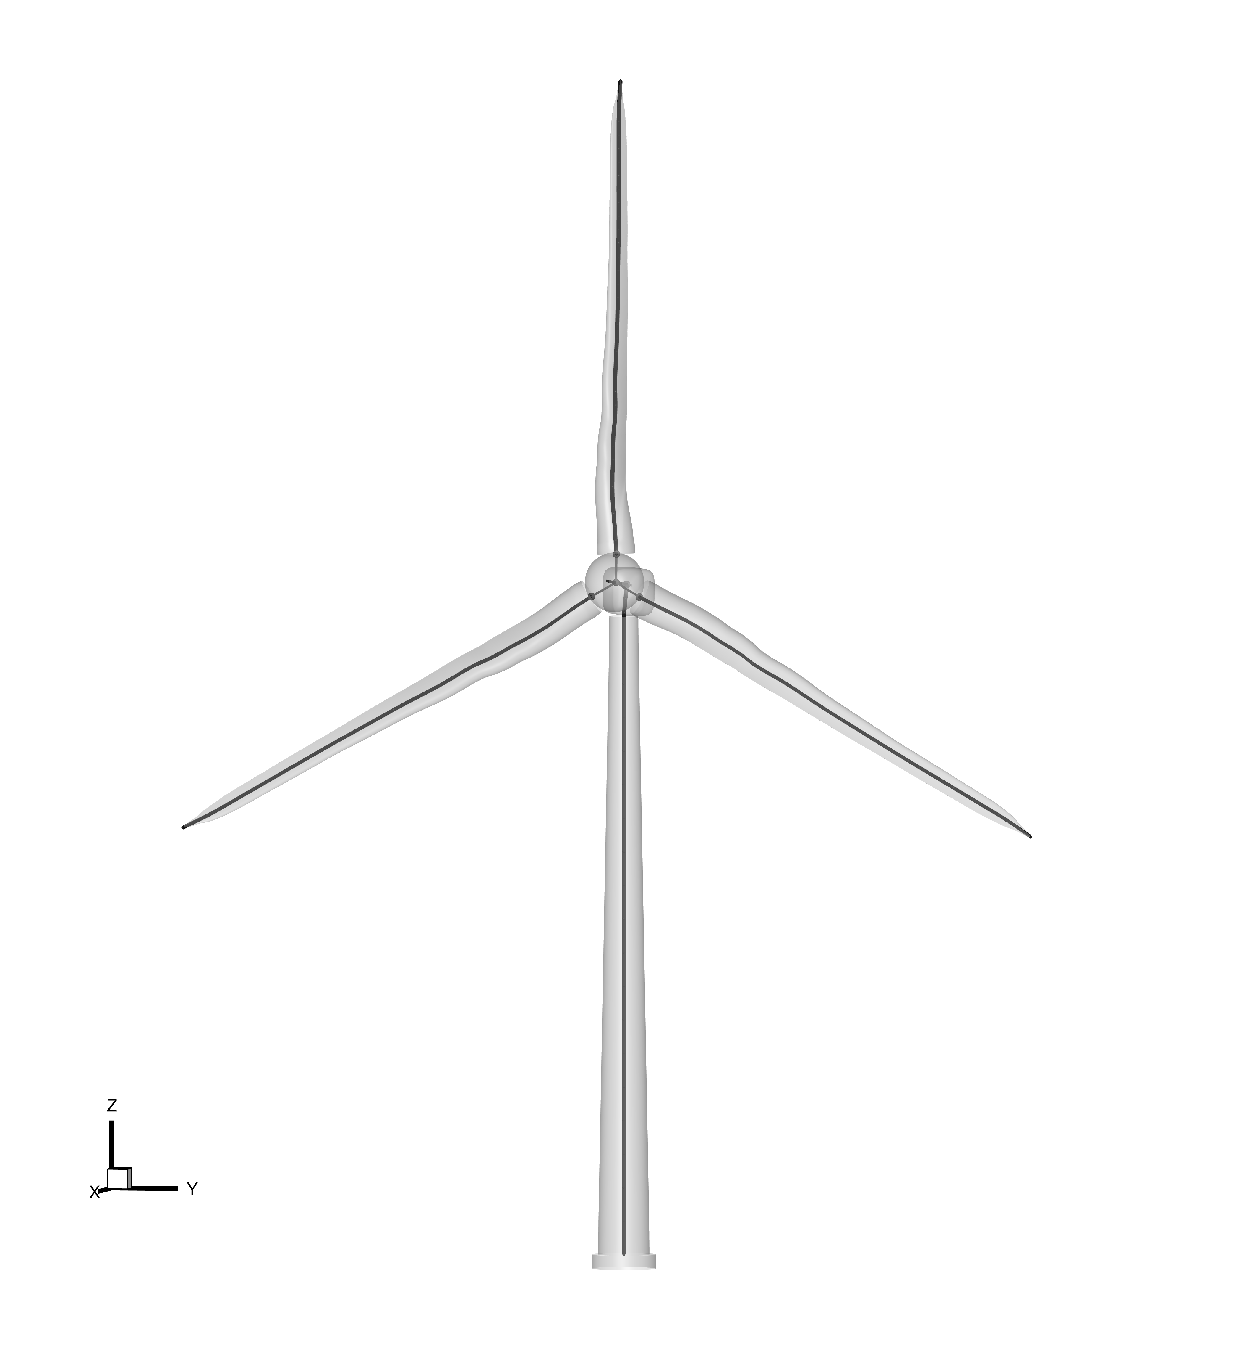
\includegraphics[width=.96\linewidth,height=.50\textheight,keepaspectratio]{figures/tecplot/turbina_3d.pdf}
\caption[Componentes del aerogenerador y eje nominal del rotor]{Vista tridimensional del aerogenerador y su idealización estructural. Las líneas y los nodos interiores corresponden a las vigas del modelo existente; las envolventes de torre, palas, góndola y cubo facilitan su identificación. Los perfiles de pala y las carcasas son ilustrativos: no proceden de un modelo CAD ni de una discretización de sólidos. Se conservan las coordenadas nodales y la conectividad del modelo.}\label{fig:turbina}
\end{figure}

\begin{figure}[htbp]
\centering
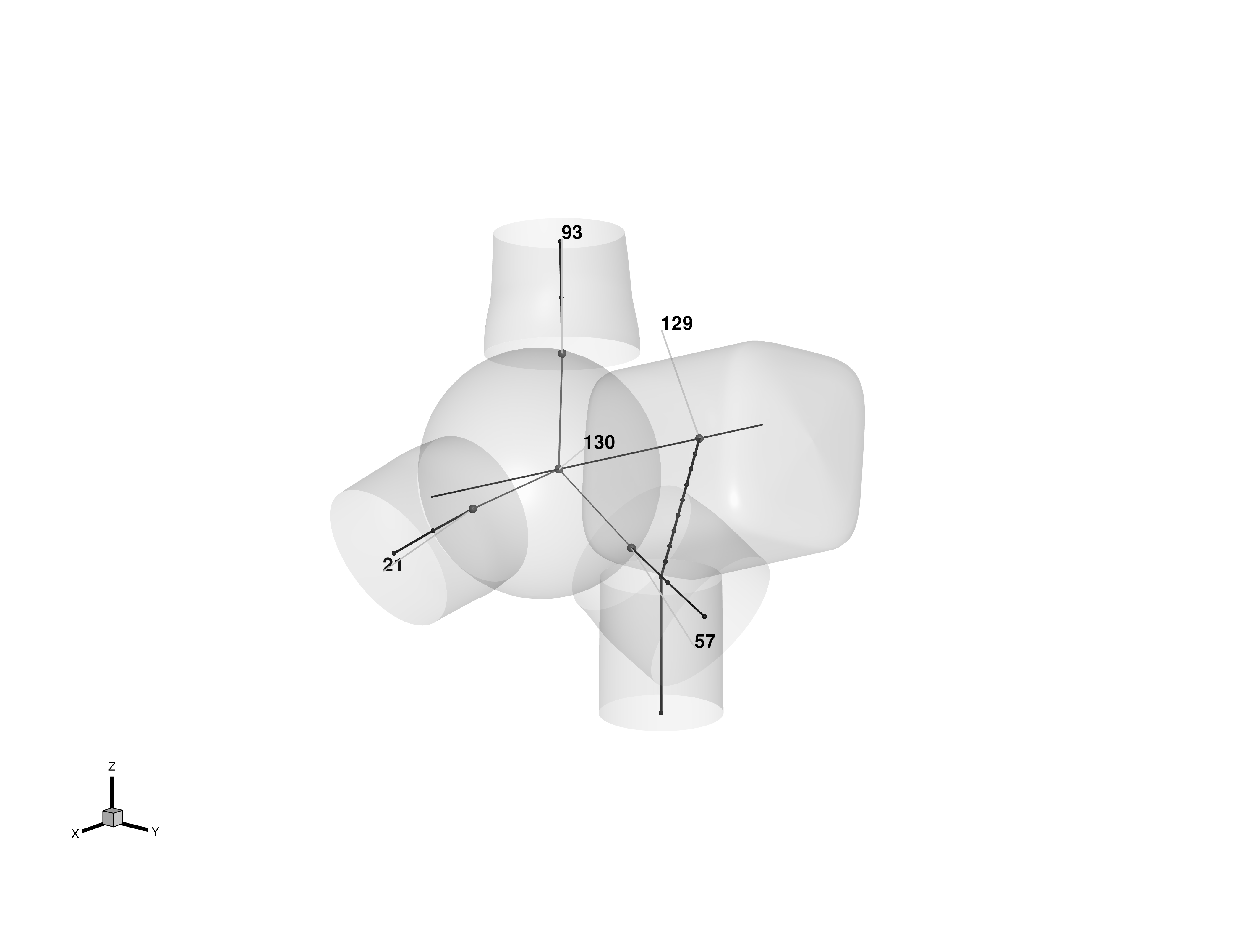
\includegraphics[width=.94\linewidth,height=.38\textheight,keepaspectratio]{figures/tecplot/turbina_conexiones_3d.pdf}
\caption[Conexiones interiores del rotor]{Detalle espacial de los elementos unidimensionales dentro de la envolvente del rotor. Se identifican los nodos de góndola 129, cubo 130 y raíces 21, 57 y 93. Las relaciones de raíz se imponen mediante compatibilidad cinemática; las envolventes son ilustrativas.}
\label{fig:conexiones3d}
\end{figure}


\section{Idealizaciones de los componentes}
La torre y cada pala se modelan mediante una línea de referencia y un triedro de sección. Las secciones pueden trasladarse y rotar; se admite deformación axial, cortante, torsión y flexión en dos planos. Esta descripción es de tipo Timoshenko en su especialización lineal. Que la sección sea rígida en su plano no significa que toda la viga sea rígida: la variación de posición y orientación de una sección a otra produce deformación.

La góndola y el conjunto cubo--nariz se idealizan como cuerpos rígidos diferentes. Cada uno posee masa, centro de masa y tensor de inercia propios. La sección superior de la torre se conecta a la góndola, y la unión entre la góndola y el cubo se representa mediante una ley elástica para los movimientos relativos de perturbación. Las raíces de las palas quedan unidas rígidamente al cubo, con la separación geométrica definida por sus brazos de conexión. El giro nominal del rotor se prescribe independientemente de estas perturbaciones.

En la presente descripción, la base sigue una traslación conocida y no una rotación impuesta. Una cimentación flexible puede representarse mediante relaciones adicionales entre acciones y desplazamientos. Sin embargo, un resorte equivalente no constituye por sí mismo un modelo continuo del suelo ni identifica sus propiedades. Para estudiar el suelo como cuerpo deformable sería necesario añadir su dominio, cinemática y ley constitutiva.

\section{Movimiento nominal y excitaciones}
La velocidad de operación se prescribe por
\begin{equation}
 \psi(t)=\psi_0+\Omega t,\qquad \dot\psi=\Omega,\qquad \ddot\psi=0.
 \label{eq:psi}
\end{equation}
El ángulo $\psi$ puede crecer sin límite; la aproximación de pequeña perturbación no se aplica a ese ángulo. La velocidad $\Omega$ tiene unidades de $\mathrm{rad/s}$ y es un dato, no una incógnita obtenida del equilibrio de pares. Si se proporciona una velocidad $n$ en revoluciones por minuto, $\Omega=2\pi n/60$.

Una \emph{operación prescrita} significa que se impone la evolución de una variable cinemática. El par necesario para mantenerla puede ser distinto de cero. El motor, generador o mecanismo ideal que sostiene el giro suministra o extrae la potencia requerida, aunque su dinámica de control no se resuelva. Por tanto, prescribir velocidad no equivale a imponer ausencia de acciones en el eje.

La dirección nominal del viento se considera fija y el eje del rotor permanece alineado con ella. La góndola mantiene una orientación nominal constante; por tanto, el movimiento de guiñada no forma parte de la operación prescrita. Las variaciones de velocidad del viento se representan mediante las cargas externas. Las pequeñas rotaciones estructurales de la góndola y el cubo pertenecen a la respuesta vibratoria y se distinguen de una maniobra de orientación.

La excitación sísmica se describe mediante una traslación conocida de la base. Las cargas aerodinámicas se introducen como fuerzas y momentos distribuidos sobre la torre y las palas. Su expresión admite dependencia de la configuración, de la velocidad estructural y del tiempo. La formulación estructural utiliza estas acciones y sus derivadas respecto del estado; un cálculo acoplado del flujo requiere, adicionalmente, las ecuaciones y condiciones de contorno del problema aerodinámico.

\section{Hipótesis de la representación estructural}
Los componentes se describen en un espacio euclídeo tridimensional. La torre y las palas se consideran esbeltas, de modo que su respuesta global puede representarse mediante variables definidas sobre una línea y propiedades integradas en la sección transversal. Quedan fuera de esta representación los fenómenos locales de pared, la delaminación y las concentraciones tridimensionales de tensiones en las uniones.

La cinemática se establece con rotaciones finitas para conservar exactamente el giro nominal. Las vibraciones se describen mediante pequeñas perturbaciones respecto del estado de operación, y las deformaciones elásticas se suponen pequeñas. Esta distinción permite que una pala complete una revolución sin aplicar la aproximación de ángulo pequeño a su azimut. La aproximación lineal se refiere al movimiento relativo de deformación, no a la trayectoria absoluta.

La geometría de referencia especifica la forma y orientación inicial de las secciones. Sus variaciones, la curvatura inicial y la torsión geométrica se describen mediante las propiedades y orientaciones de los tramos. El paso de pala y el ángulo de cono son constantes cuando pertenecen a la geometría de montaje. Los elementos rectos aproximan esta geometría por segmentos, conservando las conexiones entre componentes.

\chapter{Cinemática del aerogenerador}
\label{ch:cinematica}
\section{Cuerpo material, configuración y movimiento}
\subsection{Cuerpo material y descripción del movimiento}
Un cuerpo material $\mathcal B$ es un conjunto de partículas cuya identidad se conserva durante el movimiento. Una partícula no se define por la posición que ocupa en un instante: puede cambiar de posición sin dejar de ser la misma partícula. La torre, cada pala y cada pieza rígida se consideran cuerpos distintos. El sistema completo es una colección de cuerpos con interfaces y vínculos; las partículas de dos cuerpos conectados no se identifican entre sí por compartir una posición en la unión.

Una configuración asigna a cada partícula un punto del espacio euclídeo. La configuración de referencia se denota $\mathcal B_0$ y permite etiquetar una partícula por su posición $\vct X$. La configuración actual, $\mathcal B_t$, es el lugar que ocupa el cuerpo en el instante $t$ y usa posiciones $\vct x$. Esta distinción material--espacial, habitual en mecánica del continuo \cite{holzapfel}, permite describir el movimiento como
\begin{equation}
 \vct x=\vct\chi(\vct X,t),\qquad
 \vct\chi(\cdot,t):\mathcal B_0\longrightarrow\mathcal B_t.
 \label{eq:chi}
\end{equation}
La letra $\vct X$ identifica una posición de referencia, no un sistema de coordenadas. La misma $\vct X$ aparece para una partícula a lo largo de toda su trayectoria. En cambio, $\vct x$ depende del tiempo. Se exige localmente que el movimiento sea diferenciable e invertible y que conserve la orientación del material.

\subsection{Configuración de referencia y ausencia de tensiones}
La elección de $\mathcal B_0$ es parte de la descripción. Puede coincidir con una geometría de fabricación, una geometría descargada o una geometría precargada conocida. No es automáticamente una configuración sin tensiones. Si se adopta una geometría descargada y una ley constitutiva que asigna tensión nula a deformación nula, ambas propiedades coinciden por hipótesis, no por definición.

Para esta tesis, se toma como referencia geométrica la torre y las palas con su forma nominal de montaje, en un azimut seleccionado. La precurvatura y la pretorsión, si se incluyen, pertenecen a esa geometría inicial y no deben producir tensiones elásticas por sí solas. La deformación debida a cargas de operación se calcula respecto a ella. Esta elección debe mantenerse al interpretar las propiedades geométricas, las longitudes y las orientaciones de sección.

La figura~\ref{fig:configs} representa esta correspondencia material y permite leer el desplazamiento como la diferencia de dos posiciones medidas desde el mismo origen.

\begin{figure}[htbp]
\centering
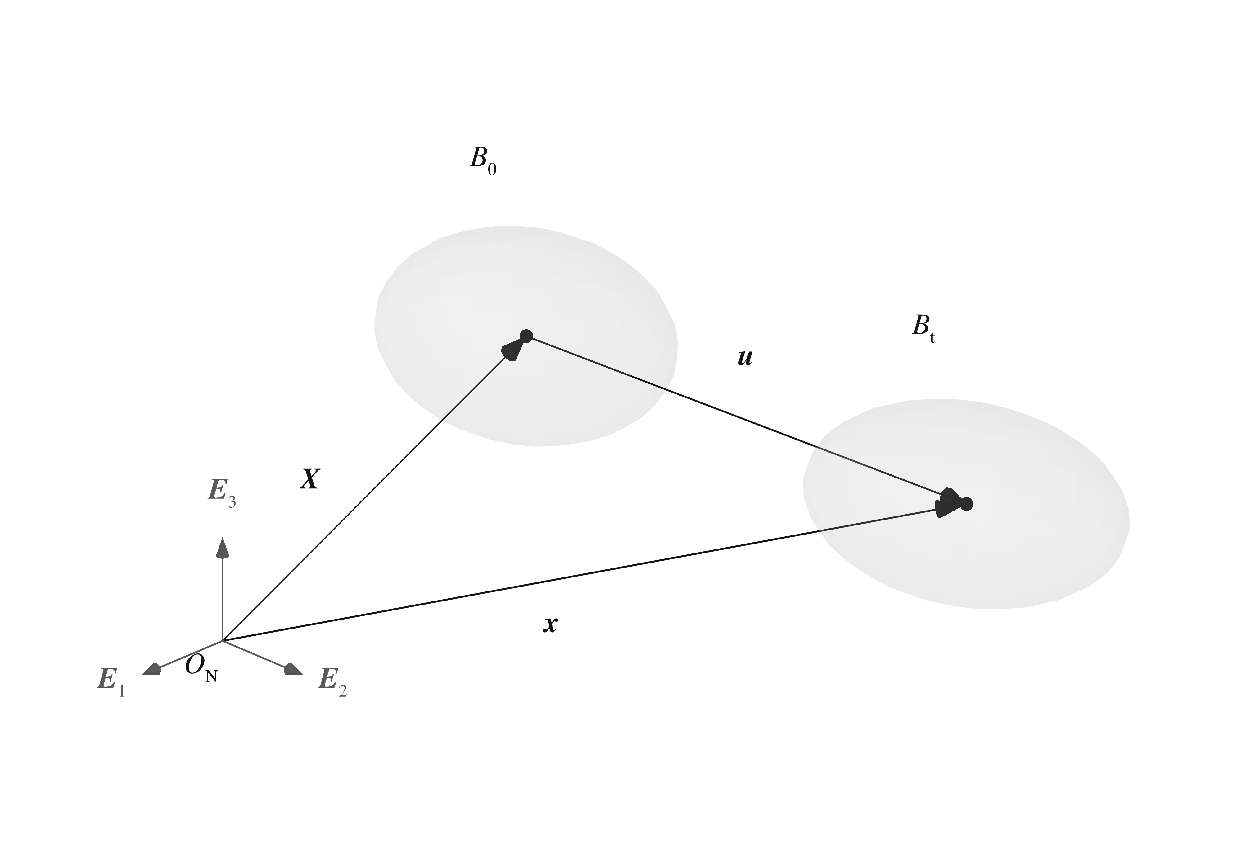
\includegraphics[width=.96\linewidth,height=.40\textheight,keepaspectratio]{figures/tecplot/concept_configs.pdf}
\caption[Configuraciones de referencia y actual]{Una misma partícula en las configuraciones de referencia y actual. Los vectores $\vct X$ y $\vct x$ se miden desde $O_N$ y su diferencia define $\vct u$. Las envolventes transparentes identifican el cuerpo material; la geometría es ilustrativa.}\label{fig:configs}
\end{figure}

\subsection{Desplazamiento y movimiento de cuerpo rígido}
En un origen y una base comunes, el desplazamiento material es
\begin{equation}
 \vct u(\vct X,t)=\vct\chi(\vct X,t)-\vct X.
\end{equation}
Incluye traslaciones y rotaciones rígidas. Por ejemplo, $\vct\chi=\vct c(t)+\ten Q(t)\vct X$ describe un movimiento rígido si $\ten Q^\tr\ten Q=\Id$ y $\det\ten Q=1$. Entonces $\vct u=\vct c+(\ten Q-\Id)\vct X$ puede ser grande, pero las distancias entre partículas no cambian. Por ello no se usa el tamaño del desplazamiento inercial como medida directa de la deformación de una pala en giro.

\section{Herramientas tensoriales y convención de componentes}
\subsection{Vectores, tensores y productos}
Un vector geométrico se escribe $\vct a$ y un tensor de segundo orden $\ten A$. En una base ortonormal dextrógira $\{\vct e_i\}$,
\begin{equation}
 \vct a=a_i\vct e_i,\qquad \ten A=A_{ij}\vct e_i\otimes\vct e_j.
\end{equation}
Se suman los índices repetidos de 1 a 3. El producto diádico se define por $(\vct a\otimes\vct b)\vct c=\vct a(\vct b\cdot\vct c)$. El producto escalar de tensores es $\ten A:\ten B=\operatorname{tr}(\ten A^\tr\ten B)$. La identidad satisface $\Id\vct a=\vct a$.

Para una terna de componentes $\vct a=(a_1,a_2,a_3)^\tr$, se define
\begin{equation}
 \sk a=\begin{bmatrix}0&-a_3&a_2\\a_3&0&-a_1\\-a_2&a_1&0\end{bmatrix},
 \qquad \sk a\vct b=\vct a\times\vct b,
 \qquad \sk a^\tr=-\sk a.
 \label{eq:skew}
\end{equation}
El símbolo $[\cdot]_\times$ es una aplicación que asocia a un vector una matriz antisimétrica. Su inversa sobre matrices antisimétricas se denota $\ax$. No es una fuerza ni una rigidez; es una herramienta para representar productos vectoriales.

\subsection{Sistema de referencia y cambio de componentes}
Un sistema de referencia $\mathcal F_A$ consta de un origen $O_A$ y una base ortonormal $\{\vct e_i^A\}$. Para expresar un vector en esa base se escribe ${}^A\vct a$. La matriz ${}^A Q_B$ contiene en sus columnas los ejes de $B$ expresados en $A$:
\begin{equation}
 ({}^A Q_B)_{ij}=\vct e_i^A\cdot\vct e_j^B,
 \quad {}^A\vct a={}^A Q_B\,{}^B\vct a,
 \quad {}^B Q_A=({}^A Q_B)^\tr.
 \label{eq:componentes}
\end{equation}
La composición respeta el orden de los sistemas de referencia: ${}^A Q_C={}^A Q_B{}^B Q_C$. Para un tensor físico,
\begin{equation}
 [\ten A]^A={}^A Q_B[\ten A]^B({}^A Q_B)^\tr.
\end{equation}
Cambiar componentes no cambia el vector físico. En contraste, aplicar una rotación física a un cuerpo modifica sus directores y posiciones. Aunque ambas operaciones se representen por matrices ortogonales, su interpretación es distinta.

La figura~\ref{fig:cambio-componentes} permite leer geométricamente la ecuación~\eqref{eq:componentes}. Las proyecciones sobre cada par de ejes producen números diferentes, pero todas representan el mismo vector. La rotación de la base no debe confundirse con el desplazamiento de una partícula.
\begin{figure}[htbp]
\centering
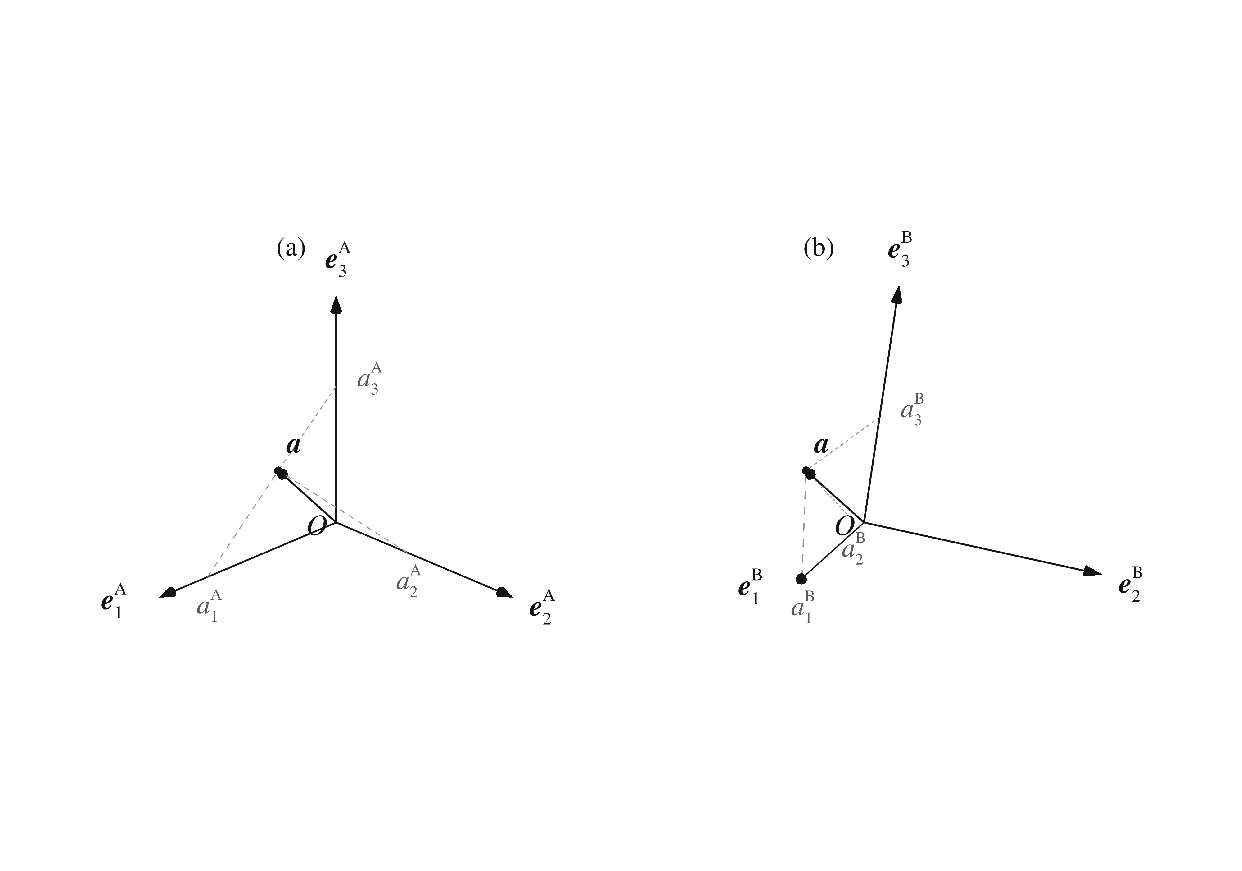
\includegraphics[width=.96\linewidth,height=.40\textheight,keepaspectratio]{figures/tecplot/concept_cambio-componentes.pdf}
\caption[Componentes de un vector en dos bases]{Un mismo vector espacial $\vct a$ expresado en las bases $A$ y $B$, representadas por separado en (a) y (b). Las líneas auxiliares relacionan la punta con sus proyecciones sobre cada eje. Cambian las componentes $a_i^A$ y $a_i^B$, mientras se conserva el vector geométrico.}\label{fig:cambio-componentes}
\end{figure}

Para una posición debe incluirse también la traslación del origen:
\begin{equation}
 {}^A\vct x={}^A\vct c_B+{}^A Q_B{}^B\vct y,
 \label{eq:affine}
\end{equation}
donde $\vct c_B$ une $O_A$ con $O_B$ y $\vct y$ une $O_B$ con el punto. No se traslada un vector libre, como una velocidad relativa o una fuerza, del mismo modo que una posición. La velocidad absoluta requiere además diferenciar los movimientos del origen y de la base.

Si también cambia el origen, la transformación de componentes se combina con una traslación, como muestra la figura~\ref{fig:frames}.

\begin{figure}[htbp]
\centering
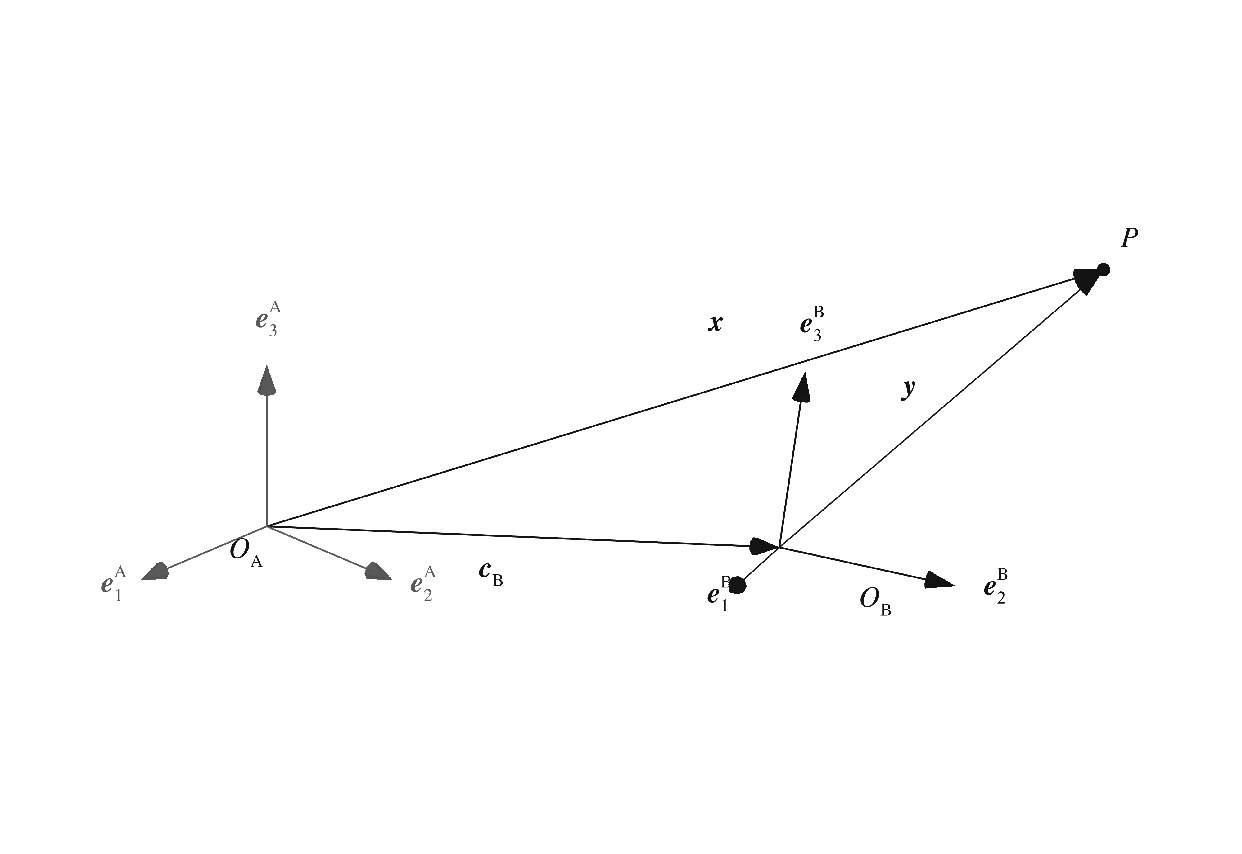
\includegraphics[width=.96\linewidth,height=.40\textheight,keepaspectratio]{figures/tecplot/concept_frames.pdf}
\caption[Cambio de origen y de base]{Cambio de origen y de base en el espacio. Los tres ejes de cada triedro permiten distinguir orientación y posición. Se cumple $\vct x=\vct c_B+\vct y$ como identidad vectorial; en componentes de $A$, ${}^A\vct x={}^A\vct c_B+{}^AQ_B{}^B\vct y$.}\label{fig:frames}
\end{figure}

\subsection{Matrices de rotación y orientación relativa}
La orientación de dos bases puede construirse mediante rotaciones elementales. Se adopta el sentido positivo de la regla de la mano derecha: el pulgar señala el eje positivo y el cierre de los dedos indica el sentido de giro. Las matrices que representan rotaciones de un vector alrededor de los ejes 1, 2 y 3 de una base ortonormal son
\begin{align}
 R_1(\alpha)&=
 \begin{bmatrix}1&0&0\\0&\cos\alpha&-\sin\alpha\\0&\sin\alpha&\cos\alpha\end{bmatrix},
 \label{eq:R1}\\
 R_2(\beta)&=
 \begin{bmatrix}\cos\beta&0&\sin\beta\\0&1&0\\-\sin\beta&0&\cos\beta\end{bmatrix},
 \label{eq:R2}\\
 R_3(\gamma)&=
 \begin{bmatrix}\cos\gamma&-\sin\gamma&0\\\sin\gamma&\cos\gamma&0\\0&0&1\end{bmatrix}.
 \label{eq:R3}
\end{align}
Cada matriz deja inalterada la componente sobre el eje de giro y transforma las dos componentes del plano perpendicular. Por ejemplo, $R_1(\alpha)\vct e_2=\cos\alpha\,\vct e_2+\sin\alpha\,\vct e_3$. Sus columnas son las imágenes de los tres vectores de la base inicial. La ortogonalidad se expresa por $R_i^\tr R_i=\Id$ y el determinante positivo conserva la orientación dextrógira.

La figura~\ref{fig:rotaciones-elementales} presenta cada rotación elemental mediante el triedro completo y el arco en el plano perpendicular a su eje. Al observar desde el semieje positivo hacia el origen, el giro positivo se ve antihorario. Las etiquetas de los ejes, y no su posición en la página, determinan qué matriz corresponde a cada panel.

\begin{figure}[htbp]
\centering
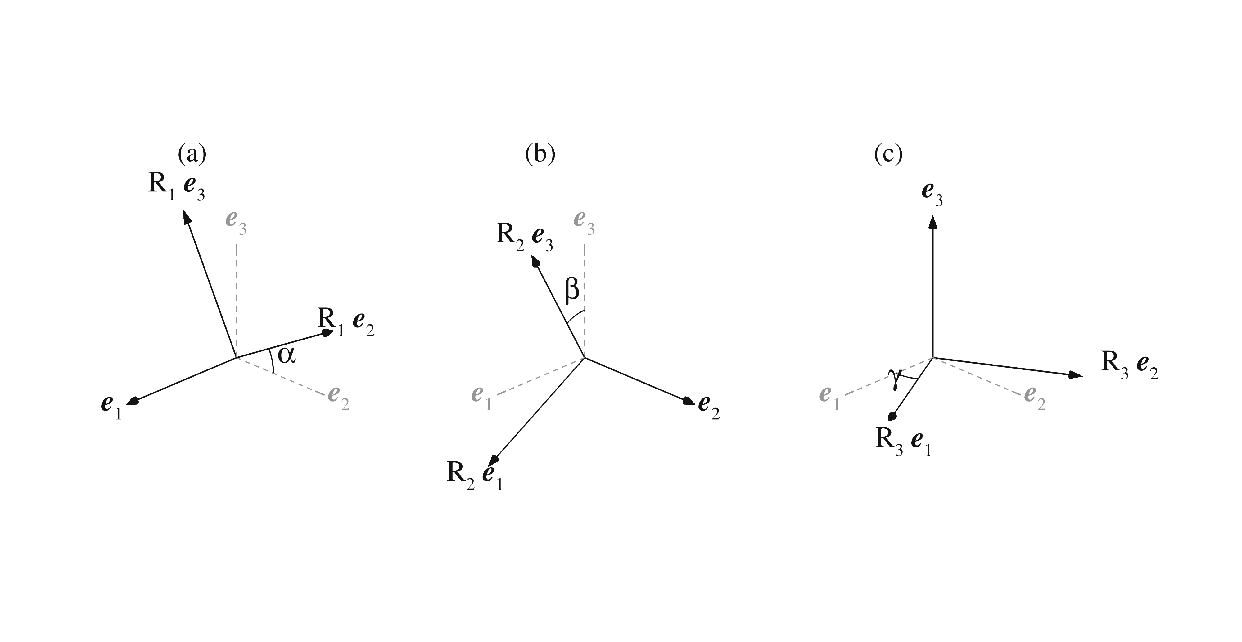
\includegraphics[width=.96\linewidth,height=.40\textheight,keepaspectratio]{figures/tecplot/concept_rotaciones-elementales.pdf}
\caption[Rotaciones elementales]{Rotaciones elementales en tres dimensiones: (a) $R_1(\alpha)$, (b) $R_2(\beta)$ y (c) $R_3(\gamma)$. Las direcciones iniciales se trazan discontinuas en gris y sus imágenes continuas en negro. El eje de giro permanece inalterado; los arcos siguen la regla de la mano derecha. Los ángulos son ilustrativos.}\label{fig:rotaciones-elementales}
\end{figure}

Si una base se obtiene girando sus propios ejes, la orientación final se construye multiplicando a la derecha la matriz de cada rotación sucesiva. Una secuencia de giros $\alpha,\beta,\gamma$ alrededor de los ejes móviles 1, 2 y 3 se representa por
\begin{equation}
 {}^A Q_B=R_1(\alpha)R_2(\beta)R_3(\gamma).
 \label{eq:cardan}
\end{equation}
Estos tres parámetros constituyen una secuencia de ángulos de Cardan. El orden forma parte de la definición: en general $R_1R_2\ne R_2R_1$. Por otra parte, expresar en $B$ las componentes de un vector conocido en $A$ requiere la matriz transpuesta $({}^AQ_B)^\tr$. Así se distinguen una rotación física, que cambia la orientación del cuerpo, y un cambio de base, que representa el mismo vector con otras componentes.

El conjunto de las matrices de rotación propias se denota
\begin{equation}
 \SO=\{Q\in\R^{3\times3}:Q^\tr Q=\Id,\ \det Q=1\}.
\end{equation}
Esta notación reúne las dos condiciones geométricas que ya se han establecido: conservación de longitudes y ángulos, y conservación de la orientación de la base.

La figura~\ref{fig:rotacion-bases} distingue la rotación de los ejes de la representación de un mismo vector en las dos bases.

\begin{figure}[htbp]
\centering
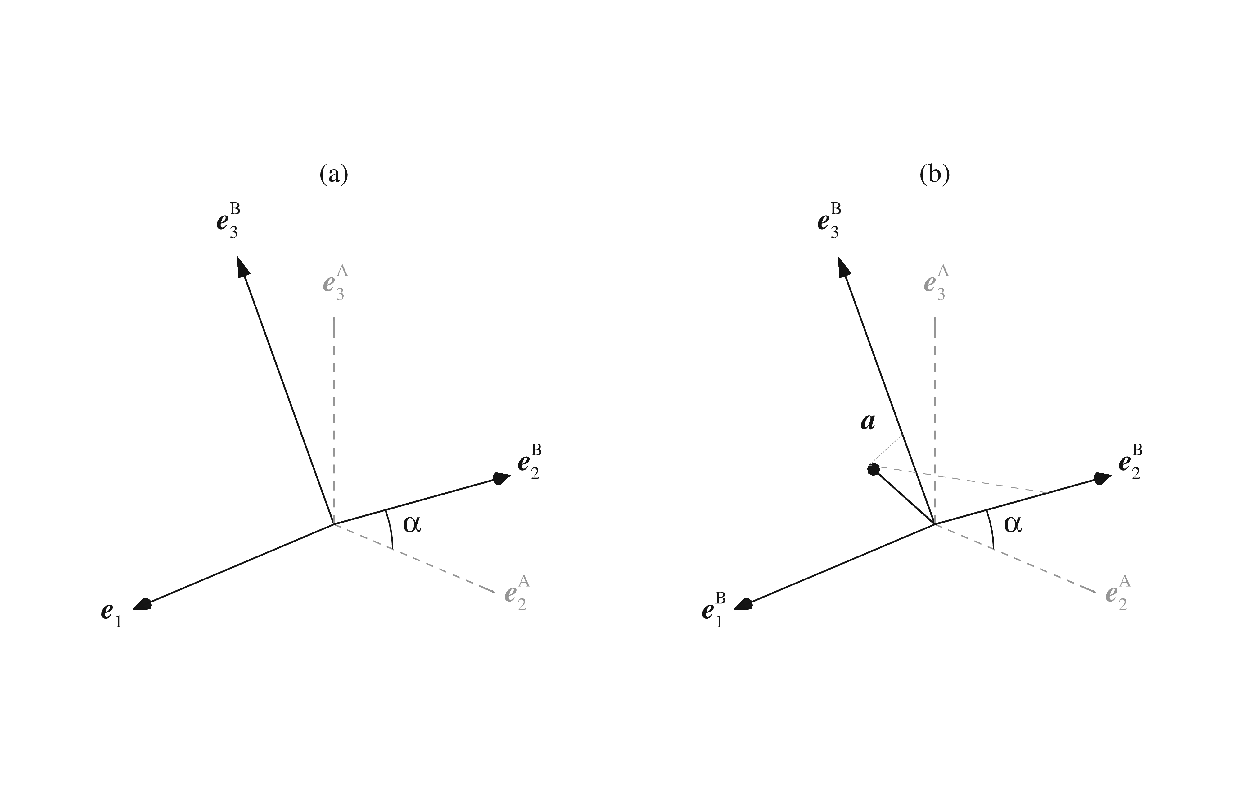
\includegraphics[width=.96\linewidth,height=.40\textheight,keepaspectratio]{figures/tecplot/concept_rotacion-bases.pdf}
\caption[Rotación de ejes y cambio de componentes]{(a) Rotación de un triedro alrededor de su eje 1. (b) Representación de un vector fijo en la base inicial y la girada. Las líneas discontinuas identifican la orientación inicial y las continuas la girada; las proyecciones se leen respecto de sus ejes respectivos. La matriz de orientación y su transpuesta tienen funciones distintas.}\label{fig:rotacion-bases}
\end{figure}

\subsection{Derivación de la velocidad angular}
La derivada de un vector de la base solidaria con un cuerpo rígido es perpendicular a ese vector. Además, la ortogonalidad entre ejes se conserva. Estas condiciones se reúnen en una única velocidad angular $\vct\omega_{B/A}$, relativa a $A$, que satisface
\begin{equation}
 \left(\frac{\dd\vct e_i^B}{\dd t}\right)_A
 =\vct\omega_{B/A}\times\vct e_i^B.
 \label{eq:derivada-ejes}
\end{equation}
El subíndice exterior indica el sistema de referencia desde el cual se deriva; el cociente $B/A$ identifica el movimiento relativo. Para $Q={}^AQ_B$, la ecuación anterior aplicada a sus tres columnas da
\begin{equation}
 \dot Q=[{}^A\vct\omega_{B/A}]_\times Q
       =Q[{}^B\vct\omega_{B/A}]_\times,\qquad
 [ {}^A\vct\omega_{B/A}]_\times=\dot Q Q^\tr.
 \label{eq:Qdot}
\end{equation}
La antisimetría también se deduce diferenciando $QQ^\tr=\Id$. Si se utiliza la transformación inversa $C=Q^\tr$, su derivada es
\begin{equation}
 \dot C=-[{}^B\vct\omega_{B/A}]_\times C.
 \label{eq:Cdot}
\end{equation}
El signo diferente corresponde a la transformación inversa y a las componentes en el sistema solidario con el cuerpo de la velocidad angular. Las dos ecuaciones describen el mismo movimiento.

Para la secuencia de \eqref{eq:cardan}, cada giro aporta una velocidad angular sobre su eje instantáneo:
\begin{equation}
 \vct\omega_{B/A}
 =\dot\alpha\,\vct e_1^A
  +\dot\beta\,\vct e_2^{(1)}
  +\dot\gamma\,\vct e_3^B.
\end{equation}
La base intermedia $(1)$ se obtiene después del primer giro. Expresando los tres ejes en la base final $B$ se obtiene
\begin{equation}
 {}^B\vct\omega_{B/A}=
 \begin{bmatrix}
 \cos\beta\cos\gamma&\sin\gamma&0\\
 -\cos\beta\sin\gamma&\cos\gamma&0\\
 \sin\beta&0&1
 \end{bmatrix}
 \begin{bmatrix}\dot\alpha\\\dot\beta\\\dot\gamma\end{bmatrix}.
 \label{eq:cardan-velocidad}
\end{equation}
Por tanto, las derivadas de los ángulos no son, en general, las componentes de la velocidad angular. La matriz de esta relación tiene determinante $\cos\beta$ y pierde invertibilidad para $\beta=\pm\pi/2$. Se trata de una singularidad de las coordenadas angulares, no de una singularidad del movimiento físico. Las matrices de orientación permiten describir el giro nominal sin recurrir a la inversión de esta relación; las perturbaciones pequeñas se parametrizan más adelante mediante un vector de rotación.

La figura~\ref{fig:derivada-director} interpreta la ecuación~\eqref{eq:derivada-ejes} mediante dos orientaciones próximas de un mismo director. El cambio del director es tangente a su esfera unitaria en el límite temporal. La velocidad angular no mide el cambio de longitud del eje, sino la rapidez y la dirección de su cambio de orientación.

\begin{figure}[htbp]
\centering
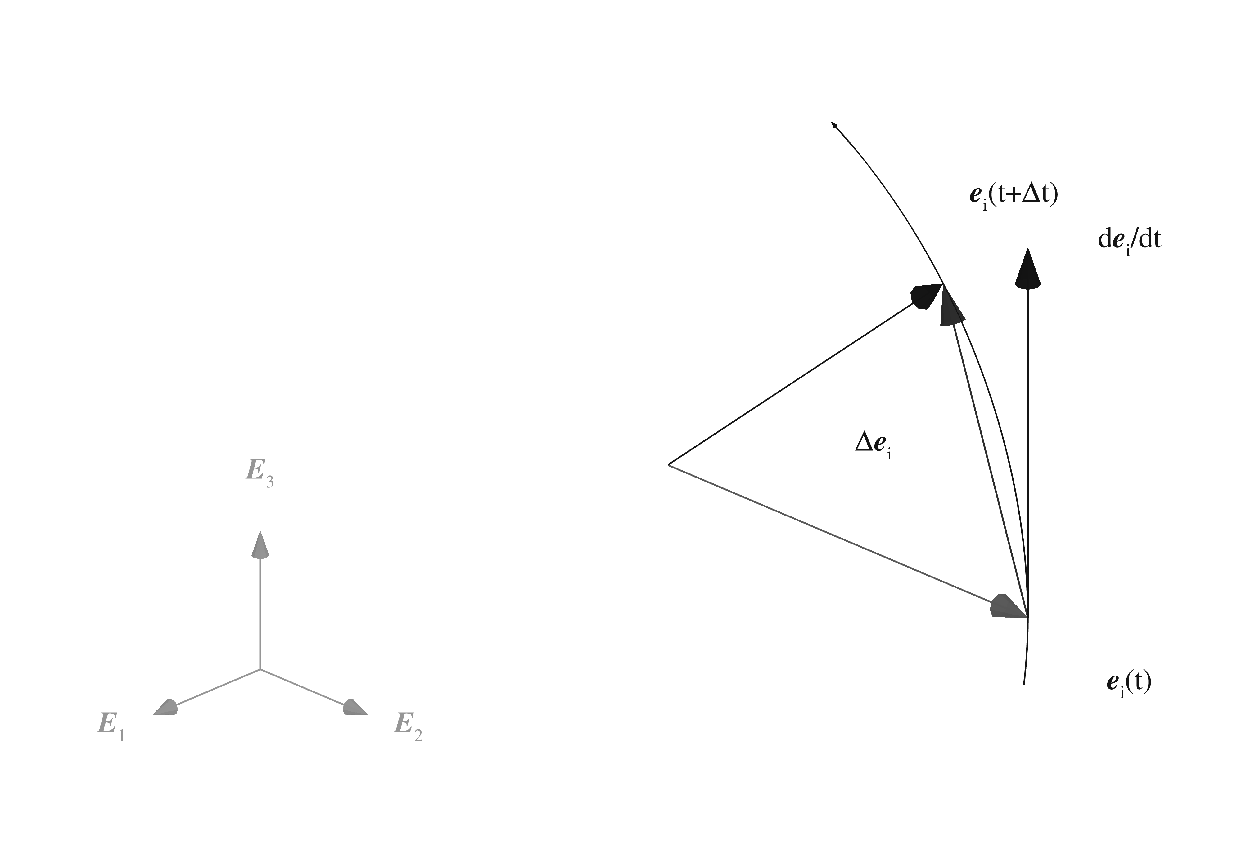
\includegraphics[width=.96\linewidth,height=.40\textheight,keepaspectratio]{figures/tecplot/concept_derivada-director.pdf}
\caption[Derivada temporal de un director]{Evolución espacial de un director de longitud constante. La cuerda une $\vct e_i(t)$ y $\vct e_i(t+\Delta t)$ y representa $\Delta\vct e_i$; la derivada en $t$ es tangente a la trayectoria circular y perpendicular al director. Las longitudes se amplían para mostrar su relación geométrica.}\label{fig:derivada-director}
\end{figure}

\subsection{Derivada de un vector en una base móvil}
Sea $\vct a=a_i^B(t)\vct e_i^B(t)$. Al aplicar la regla de derivación del producto,
\begin{equation}
 \left(\frac{\dd\vct a}{\dd t}\right)_A
 =\dot a_i^B\vct e_i^B+
   a_i^B\left(\frac{\dd\vct e_i^B}{\dd t}\right)_A
 =\left(\frac{\dd\vct a}{\dd t}\right)_B+
   \vct\omega_{B/A}\times\vct a.
 \label{eq:teorema-transporte}
\end{equation}
Esta identidad es el teorema de transporte de la derivada de un vector. Su primer término representa el cambio de las componentes medidas en $B$; el segundo representa el cambio de la base. Para un vector fijo en el cuerpo, el primer término es nulo, aunque la derivada observada desde $A$ no lo sea. Para una pala flexible, en cambio, sus vectores de posición relativos varían también por deformación y ambos términos intervienen.

La composición de orientaciones $ {}^NQ_P={}^NQ_H{}^HQ_P$, al ser derivada y multiplicada por su transpuesta, conduce a la composición de velocidades angulares
\begin{equation}
 {}^N\vct\omega_{P/N}
 ={}^N\vct\omega_{H/N}
  +{}^NQ_H\,{}^H\vct\omega_{P/H}.
 \label{eq:composicion-omega}
\end{equation}
Las velocidades angulares se suman como vectores una vez expresadas en una base común. Esta propiedad no implica que puedan sumarse del mismo modo los ángulos de rotaciones finitas.

\section{Medidas de deformación del continuo}
La derivada material del movimiento es el gradiente de deformación:
\begin{equation}
 \ten F=\Grad_{\!X}\vct\chi,
 \qquad \dd\vct x=\ten F\dd\vct X,
 \qquad J=\det\ten F>0.
\end{equation}
El tensor $\ten F$ transporta segmentos infinitesimales desde la configuración de referencia a la actual; no es simplemente una matriz de rotación. Es un tensor de dos puntos: su argumento pertenece al espacio tangente material y su imagen al espacial. En componentes, $F_{iA}=\partial x_i/\partial X_A$; el índice mayúsculo identifica el lado material, no una potencia. El escalar $J$ mide la razón local de volumen, $\dd V=J\dd V_0$. Para masa conservada, $\rho J=\rho_0$. El símbolo $J$ sin índice no se usa aquí para el tensor de inercia, que se escribe $\ten J_C$.

Al comparar longitudes se obtiene
\begin{align}
 \dd\vct x\cdot\dd\vct x&=\dd\vct X\cdot\ten C\dd\vct X,
 &\ten C&=\ten F^\tr\ten F,\\
 \ten E&=\tfrac12(\ten C-\Id),
 &\|\dd\vct x\|^2-\|\dd\vct X\|^2&=2\dd\vct X\cdot\ten E\dd\vct X.
\end{align}
Aquí $\ten E$ es la deformación de Green--Lagrange. Para un movimiento rígido $\ten F=\ten Q$, se tiene $\ten C=\Id$ y $\ten E=\ten0$. Esta comprobación distingue una descripción geométricamente consistente de una que interpreta el giro como deformación.

Si $\ten H=\Grad\vct u$, la identidad exacta es
\begin{equation}
 \ten E=\tfrac12(\ten H+\ten H^\tr+\ten H^\tr\ten H).
\end{equation}
Solo cuando el gradiente de desplazamiento es pequeño puede despreciarse el último término. En el rotor, el giro nominal grande debe separarse antes de aplicar esa aproximación. Linealizar directamente el desplazamiento total inercial a lo largo de una revolución generaría deformaciones ficticias.

La descomposición polar $\ten F=\ten R\ten U=\ten V\ten R$ separa una rotación de un estiramiento, con $\ten R\in\SO$ y $\ten U$, $\ten V$ simétricos positivos. No debe confundirse esa rotación polar del continuo con la rotación de un triedro de sección: en una viga con cortante, el director longitudinal no coincide necesariamente con la tangente a la línea media ni con la rotación polar local.

\subsection{Dos movimientos que permiten interpretar las medidas}
Para un bloque que gira rígidamente un ángulo $\alpha$ en el plano 1--2, $\ten F=R_3(\alpha)$ y $\ten E=0$. Sin embargo, si se aplicara la medida infinitesimal al desplazamiento total, se obtendría
\begin{equation}
 \sym\Grad\vct u=\sym(R_3(\alpha)-\Id)
 =\diag(\cos\alpha-1,\cos\alpha-1,0).
\end{equation}
Para un ángulo finito esta matriz no es cero: el resultado no revela una deformación física, sino el uso de una aproximación fuera de su dominio. Esto justifica separar el giro nominal del rotor antes de introducir una deformación lineal.

En cambio, el movimiento $x_1=X_1+kX_2$, $x_2=X_2$, $x_3=X_3$ es un cortante simple. Su gradiente y su medida de Green--Lagrange son
\begin{equation}
 F=\begin{bmatrix}1&k&0\\0&1&0\\0&0&1\end{bmatrix},\qquad
 E=\frac12\begin{bmatrix}0&k&0\\k&k^2&0\\0&0&0\end{bmatrix}.
\end{equation}
Se conserva el volumen porque $\det F=1$, pero cambian ángulos y longitudes. Una fibra inicialmente paralela al eje 2 adquiere longitud multiplicada por $\sqrt{1+k^2}$. A primer orden se retiene $E_{12}=k/2$ y se desprecia $k^2/2$; esa aproximación requiere $|k|\ll1$. Ni conservación de volumen ni gran desplazamiento bastan por sí solos para identificar la deformación.

La figura~\ref{fig:rotacion-deformacion} compara ambos movimientos mediante una cuadrícula material: la rotación conserva los ángulos entre sus líneas, mientras que el cortante los modifica.

\begin{figure}[htbp]
\centering
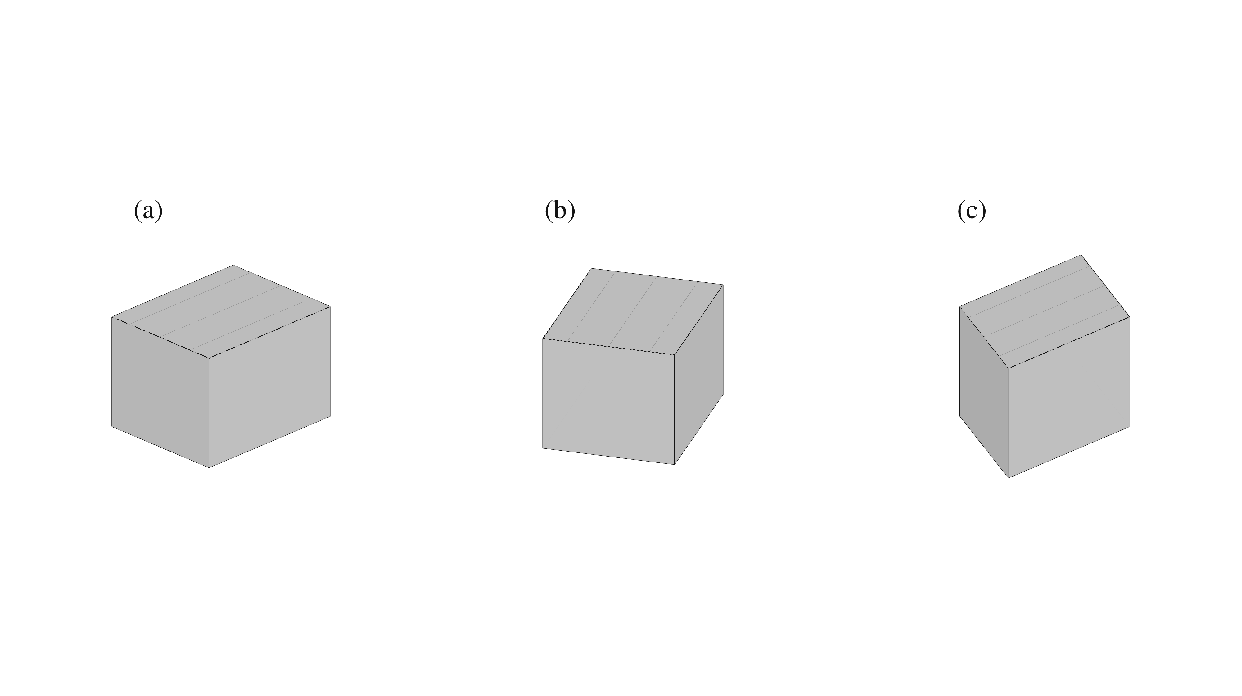
\includegraphics[width=.96\linewidth,height=.40\textheight,keepaspectratio]{figures/tecplot/concept_rotacion-deformacion.pdf}
\caption[Rotación rígida y deformación por cortante]{Una misma porción material en tres dimensiones: (a) referencia, (b) rotación rígida y (c) deformación por cortante. La cuadrícula identifica líneas materiales. La rotación conserva los ángulos y las longitudes; la deformación cambia la forma.}\label{fig:rotacion-deformacion}
\end{figure}

\section{Velocidad, aceleración y derivadas}
La velocidad y aceleración materiales se calculan manteniendo fija la etiqueta $\vct X$:
\begin{equation}
 \vct v(\vct X,t)=\left.\frac{\partial\vct\chi}{\partial t}\right|_X,
 \qquad \vct a(\vct X,t)=\left.\frac{\partial^2\vct\chi}{\partial t^2}\right|_X.
\end{equation}
Una representación espacial de la velocidad se obtiene sustituyendo $\vct X=\vct\chi^{-1}(\vct x,t)$. Para un campo espacial $\vct w(\vct x,t)$, la derivada siguiendo una partícula es
\begin{equation}
 \frac{D\vct w}{Dt}=\frac{\partial\vct w}{\partial t}+(\grad\vct w)\vct v.
\end{equation}
No se intercambia esa derivada con una derivada a posición espacial fija. El gradiente espacial de velocidad satisface $\ten l=\dot{\ten F}\ten F^{-1}$ y se separa en $\ten d=\sym\ten l$ y $\ten w=(\ten l-\ten l^\tr)/2$. El segundo es el tensor de giro local del continuo; el símbolo $\ten w$ no se identifica automáticamente con la velocidad angular prescrita del rotor.

\section{Sistemas de referencia de los componentes}
\subsection{Sistema de referencia newtoniano}
El sistema de referencia $\mathcal F_N=\{O_N;\vct E_1,\vct E_2,\vct E_3\}$ se considera inercial en la escala de tiempo del problema. Se toma $\vct E_3$ vertical, $\vct E_1$ en la dirección nominal de viento y $\vct E_2=\vct E_3\times\vct E_1$. Es una aproximación newtoniana local: no se incluyen rotación terrestre ni curvatura terrestre. Las aceleraciones absolutas empleadas en el balance de cantidad de movimiento se refieren a este sistema de referencia.

\subsection{Base y torre}
El sistema de referencia $\mathcal F_B$ tiene origen en la base de la torre y ejes paralelos a los de $N$. Su posición es $\vct c_B(t)=\vct c_{B*}+\vct u_B(t)$ y ${}^NQ_B=\Id$. Si $\ddot{\vct u}_B\ne\vct0$, es un sistema de referencia acelerado, no newtoniano. Un observador ligado a él mide posiciones relativas; la aceleración absoluta recupera el término $\ddot{\vct c}_B$.

La torre no necesita un único sistema de referencia solidario único, pues es flexible. Cada sección tiene sus directores. Como parametrización nominal se elige $S$ desde la base hacia la parte superior, con $\vct D_1=\vct E_3$, $\vct D_2=\vct E_1$ y $\vct D_3=\vct E_2$. Esta terna es dextrógira. La orientación actual de cada sección puede diferir por flexión y torsión.

\subsection{Góndola y eje nominal}
Se introduce $\mathcal F_G$ en un punto de referencia de la góndola. Su base \emph{nominal} es constante y el eje $\vct e_1^G$ define el eje del rotor. En el caso alineado y horizontal, ${}^NQ_G=\Id$; una orientación constante diferente puede representarse mediante una matriz de montaje conocida, pero no una guiñada temporal.

Es útil distinguir $\overline{\mathcal F}_G$, nominal, de $\mathcal F_G(t)$, solidario con la góndola perturbada. Su orientación puede escribirse ${}^NQ_G(t)={}^N\overline Q_G\exp(\sk{\theta_G})$. La terna $\vct\theta_G$ es pequeña y se expresa en la base nominal de la góndola. Así puede haber vibración angular de la góndola sin introducir un seguimiento nominal del viento.

\subsection{Cubo y nariz}
El origen $O_H$ está sobre el eje del rotor, en un punto de referencia del cubo. La nariz comparte el movimiento rígido del cubo cuando se idealizan como una sola pieza. La base nominal del cubo satisface
\begin{equation}
 {}^N\overline Q_H(t)={}^N\overline Q_G R_1(\psi(t)),\qquad
 R_1(\psi)=\begin{bmatrix}1&0&0\\0&\cos\psi&-\sin\psi\\0&\sin\psi&\cos\psi\end{bmatrix}.
\end{equation}
El eje 1 es el eje de giro, mientras los ejes 2 y 3 recorren el plano del rotor. La velocidad angular nominal es $\overline{\vct\omega}=\Omega\vct e_1^G$. Su dirección es fija en el sistema de referencia newtoniano bajo la hipótesis nominal adoptada.

El origen nominal $\overline{\vct c}_H(t)$ incluye la traslación de la base, la altura de la torre y la separación constante entre los puntos de referencia de la góndola y el cubo. Los desplazamientos y las rotaciones de perturbación del cubo son incógnitas estructurales. Su diferencia respecto del movimiento de la góndola determina la deformación de la conexión elástica, mientras que el azimut $\psi$ conserva su carácter prescrito.

Las figuras~\ref{fig:sistemas-lateral} y \ref{fig:cubo-nominal} separan dos vistas complementarias. La primera localiza los orígenes y los ejes nominales de los componentes estacionarios; la segunda muestra exclusivamente cómo cambia la orientación del cubo. El superíndice $H,n$ identifica la base nominal del cubo en las figuras. Las tres direcciones de cada triedro se muestran mediante flechas espaciales; las líneas discontinuas permiten distinguir la orientación inercial de la nominal.

\begin{figure}[htbp]
\centering
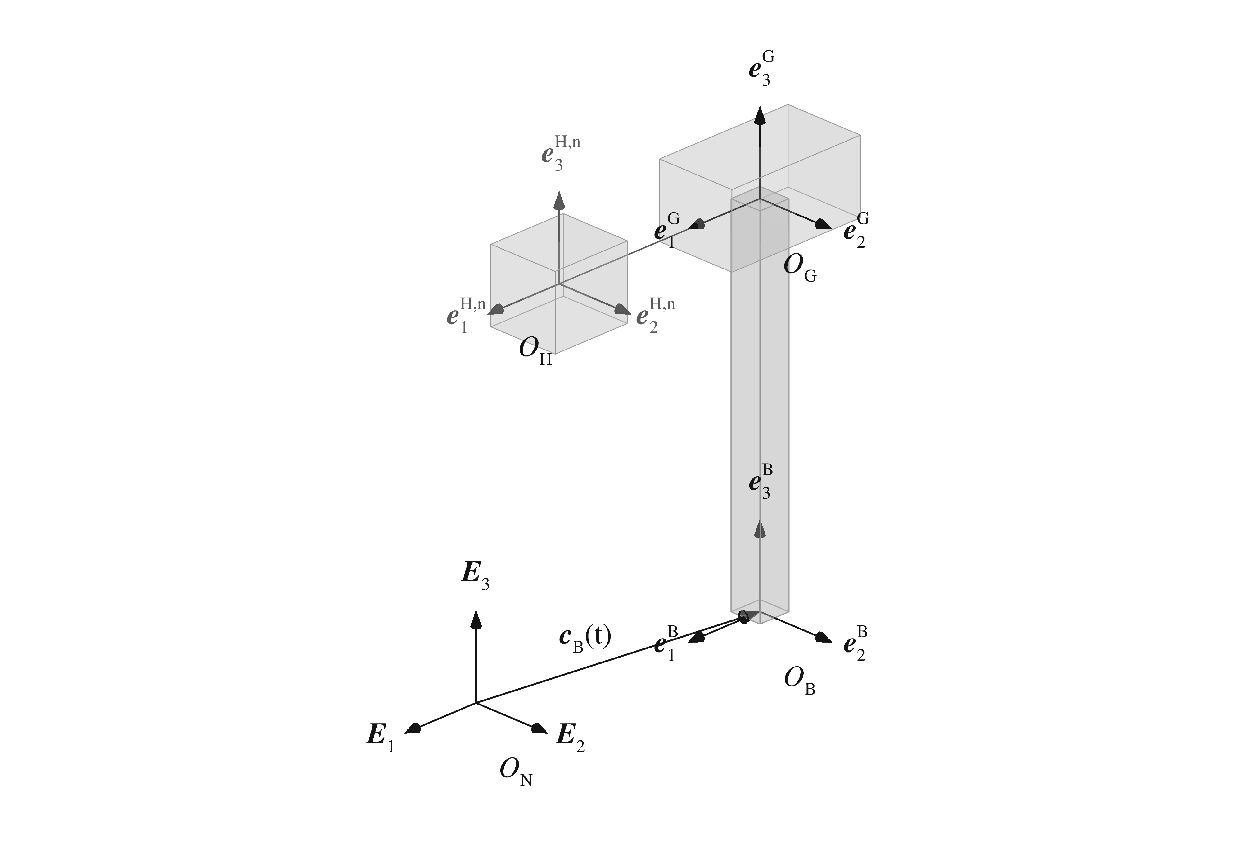
\includegraphics[width=.96\linewidth,height=.40\textheight,keepaspectratio]{figures/tecplot/concept_sistemas-lateral.pdf}
\caption[Sistemas de referencia de la base y la góndola]{Sistemas de referencia de la base, la góndola y el cubo en una vista espacial. $\vct c_B(t)$ sitúa la base respecto de $O_N$ y los triedros muestran sus tres direcciones. El superíndice $H,n$ identifica la base nominal del cubo. Los volúmenes y separaciones son esquemáticos; no representan una malla de sólidos.}\label{fig:sistemas-lateral}
\end{figure}

\begin{figure}[htbp]
\centering
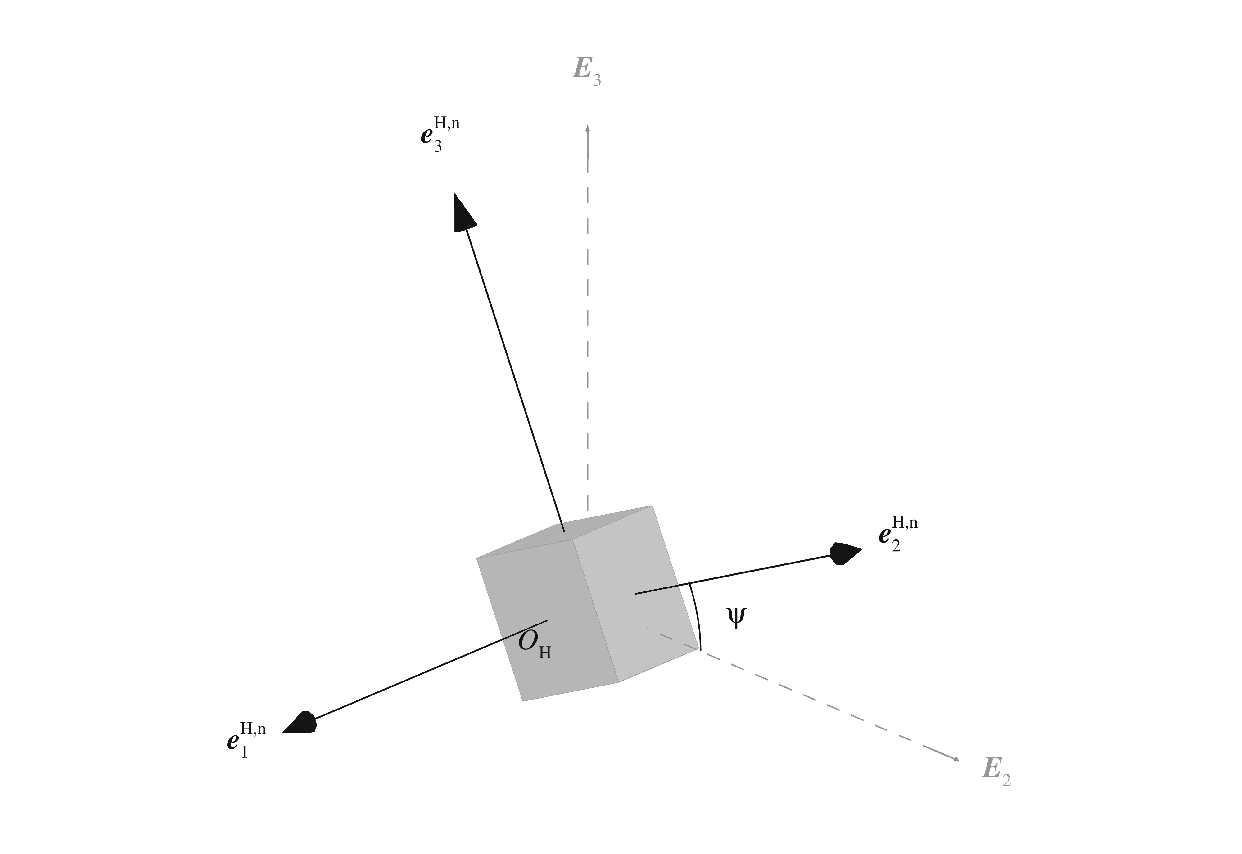
\includegraphics[width=.96\linewidth,height=.40\textheight,keepaspectratio]{figures/tecplot/concept_cubo-nominal.pdf}
\caption[Rotación nominal del cubo]{Orientación nominal del cubo en tres dimensiones. El azimut $\psi$ gira las direcciones 2 y 3 alrededor del eje 1, que permanece común. Las direcciones inerciales son discontinuas y las nominales continuas. El superíndice $H,n$ equivale a la notación $\overline{\vct e}_i^H$ del texto.}\label{fig:cubo-nominal}
\end{figure}

\subsection{Sistemas de referencia de las tres palas}
Cada pala $b\in\{1,2,3\}$ tiene un sistema de referencia de montaje $\mathcal F_{P_b}$ en su raíz. Para espaciamiento uniforme, $\beta_b=2\pi(b-1)/3$. La orientación nominal es
\begin{equation}
 {}^N\overline Q_{P_b}(t)={}^N\overline Q_H(t){}^HQ_{P_b},
 \qquad {}^HQ_{P_b}=R_1(\beta_b)Q_{\rm mont,b}.
\end{equation}
La matriz $Q_{\rm mont,b}$ establece la orientación de la sección de raíz. Para tres palas rectas sin cono ni paso inicial, se adopta la misma matriz de montaje antes de aplicar la separación angular de cada pala:
\begin{equation}
 Q_{\rm mont,b}=[\vct e_3,-\vct e_2,\vct e_1],
 \qquad\text{componentes expresadas en }H.
\end{equation}
Así, el eje 1 de cada pala es radial, el eje 2 es tangencial en el sentido de giro positivo y el eje 3 es paralelo al eje del rotor. La pala 1 coincide con el eje 3 del cubo cuando $\psi=0$; para una góndola horizontal, apunta verticalmente hacia arriba. Esta elección coincide con las vistas de las figuras~\ref{fig:turbina} y \ref{fig:cubo-brazos}.

Las direcciones nominales, expresadas en el cubo, quedan definidas por
\begin{align}
 \vct d_{1b}^H&=-\sin\beta_b\,\vct e_2+\cos\beta_b\,\vct e_3,\\
 \vct d_{2b}^H&=-\cos\beta_b\,\vct e_2-\sin\beta_b\,\vct e_3,
 &\vct d_{3b}^H&=\vct e_1.
\end{align}
En particular, las matrices de las tres palas son
\begin{align}
 {}^HQ_{P_1}&=\begin{bmatrix}0&0&1\\0&-1&0\\1&0&0\end{bmatrix},\\
 {}^HQ_{P_2}&=\begin{bmatrix}
 0&0&1\\-\sqrt3/2&1/2&0\\-1/2&-\sqrt3/2&0
 \end{bmatrix},\qquad
 {}^HQ_{P_3}=\begin{bmatrix}
 0&0&1\\\sqrt3/2&1/2&0\\-1/2&\sqrt3/2&0
 \end{bmatrix}.
 \label{eq:matrices-tres-palas}
\end{align}
Si $r_H$ es la distancia del centro del cubo a cada raíz, sus posiciones relativas son
\begin{equation}
 \vct r_{10}^H=r_H\begin{bmatrix}0\\0\\1\end{bmatrix},\quad
 \vct r_{20}^H=r_H\begin{bmatrix}0\\-\sqrt3/2\\-1/2\end{bmatrix},\quad
 \vct r_{30}^H=r_H\begin{bmatrix}0\\\sqrt3/2\\-1/2\end{bmatrix}.
 \label{eq:raices-tres-palas}
\end{equation}
Estos vectores describen posiciones, mientras que las columnas de \eqref{eq:matrices-tres-palas} describen direcciones unitarias. Multiplicar los primeros por la orientación del cubo sitúa las raíces en el espacio; multiplicar las matrices por esa orientación determina los ejes de cada pala.

La figura~\ref{fig:marcos} identifica simultáneamente las nueve direcciones locales de las tres raíces. Las tres direcciones $\vct d_{3b}^H$ coinciden con el eje del rotor; las seis direcciones restantes se leen en el plano. Los puntos de raíz son distintos aunque pertenezcan al mismo cuerpo rígido de unión.
\begin{figure}[htbp]
\centering
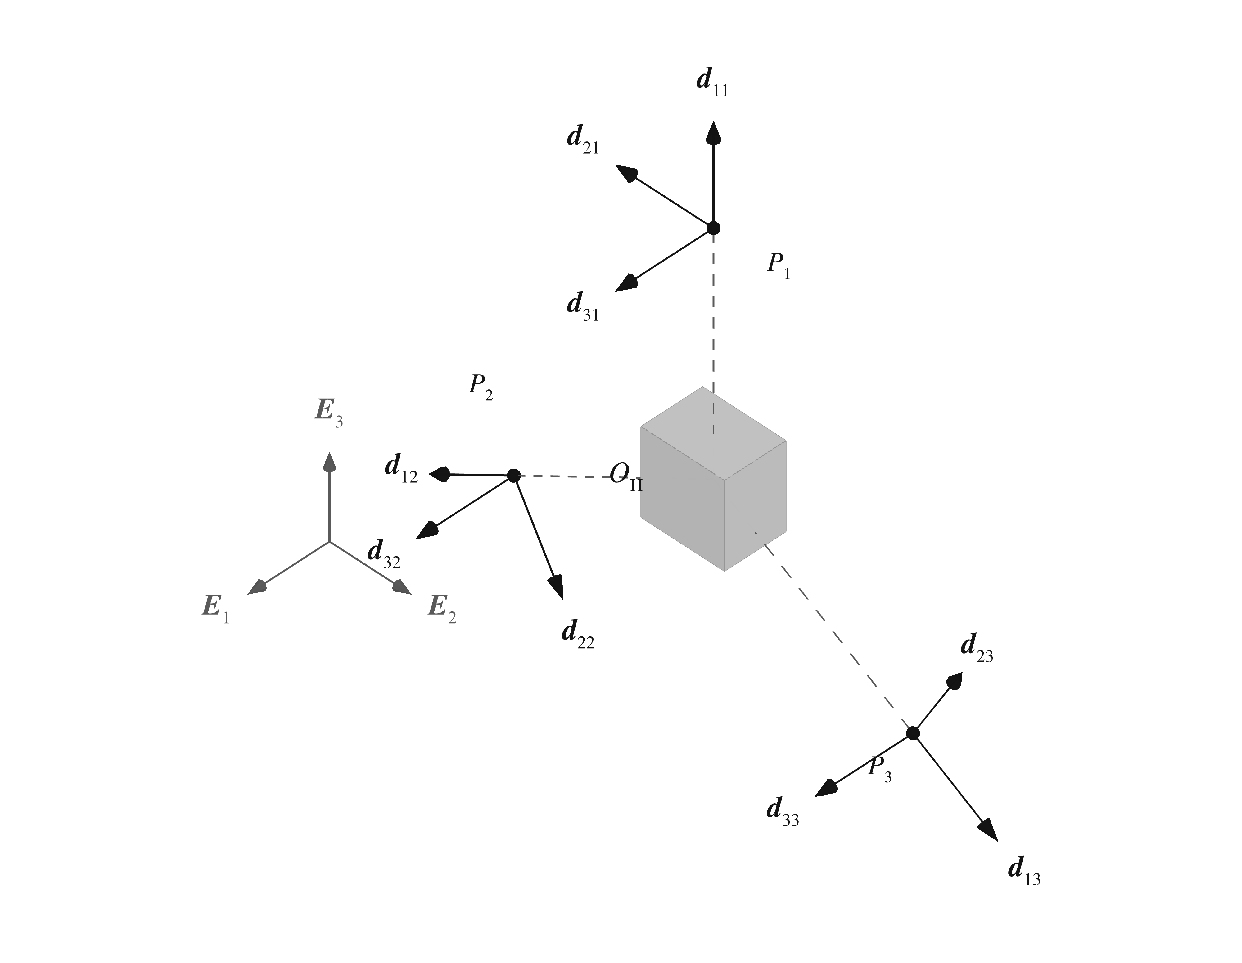
\includegraphics[width=.96\linewidth,height=.40\textheight,keepaspectratio]{figures/tecplot/concept_marcos.pdf}
\caption[Sistemas de referencia de las raíces]{Triedros de las tres raíces para azimut nominal nulo. El eje $\vct d_{1b}$ es longitudinal, $\vct d_{2b}$ tangencial y $\vct d_{3b}=\vct E_1$. Se muestran las tres direcciones, los puntos $P_b$ y el origen del cubo. Las separaciones angulares son $120^\circ$ y la perspectiva conserva la convención dextrógira.}\label{fig:marcos}
\end{figure}

Un paso fijo $\alpha_{p,b}$ se incorpora por una rotación alrededor del eje longitudinal de la pala:
\begin{equation}
 {}^HQ_{P_b}^{\,\mathrm{paso}}
 ={}^HQ_{P_b}R_1(\alpha_{p,b}).
 \label{eq:paso-fijo}
\end{equation}
El ángulo de paso orienta la sección en la raíz; la torsión geométrica describe la variación de esa orientación a lo largo de la pala; y la torsión elástica es el cambio producido por la deformación. Son tres magnitudes distintas. En el movimiento nominal adoptado, el paso es constante y no aporta una velocidad angular relativa. La torsión elástica, cuando varía con el tiempo, sí contribuye a la velocidad angular de las secciones.

La figura~\ref{fig:palas-paso} muestra el ángulo de paso en el plano de la sección, separado del azimut del rotor.

\begin{figure}[htbp]
\centering
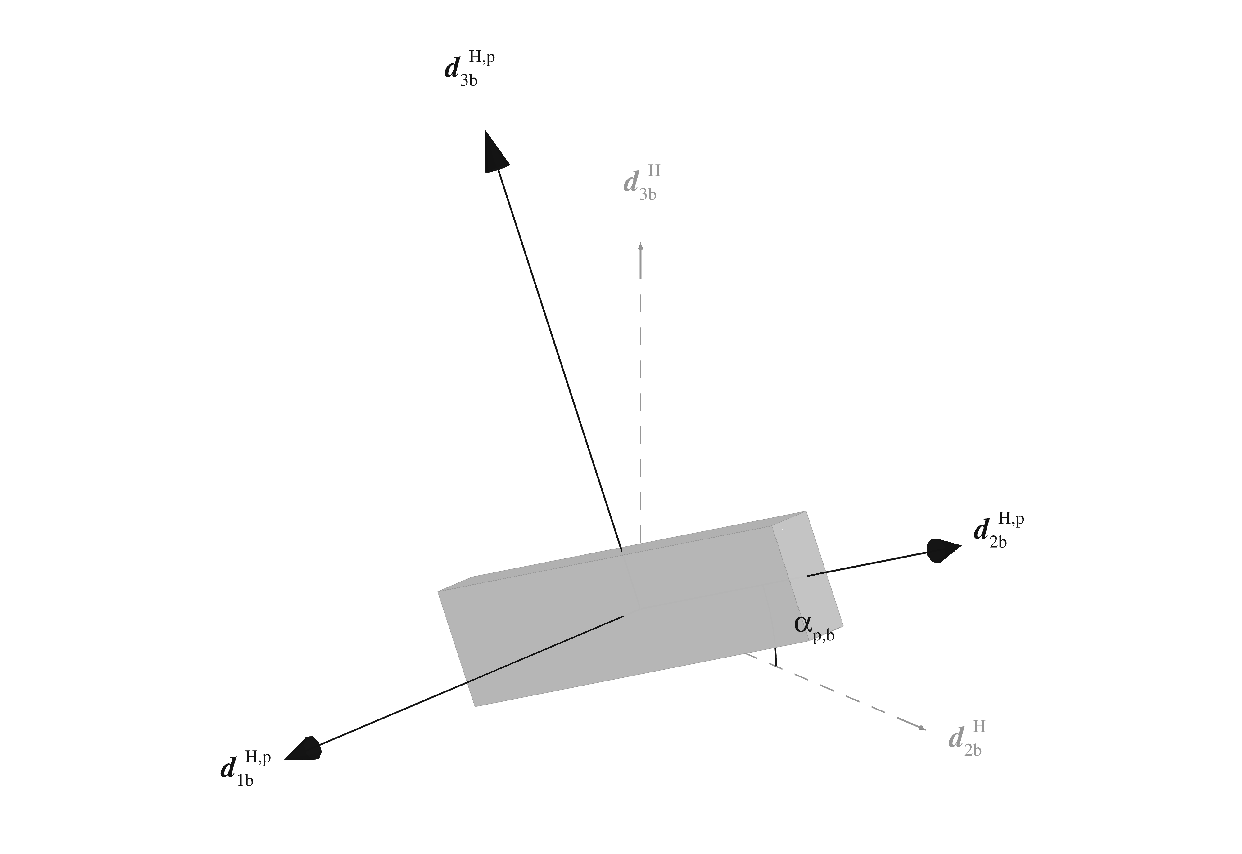
\includegraphics[width=.96\linewidth,height=.40\textheight,keepaspectratio]{figures/tecplot/concept_palas-paso.pdf}
\caption[Ángulo de paso de una sección de pala]{Rotación de paso de una sección en tres dimensiones. Las direcciones discontinuas $\vct d_{ib}^{H}$ corresponden al montaje sin paso y las continuas $\vct d_{ib}^{H,p}$ a la sección rotada. El eje longitudinal permanece común y la raíz no se traslada. El espesor de la sección facilita la lectura de su orientación.}\label{fig:palas-paso}
\end{figure}

Las relaciones entre los sistemas de referencia se reúnen en la figura~\ref{fig:arbol}; esta organización permite construir a continuación la posición absoluta de cada componente.

\begin{figure}[htbp]
\centering
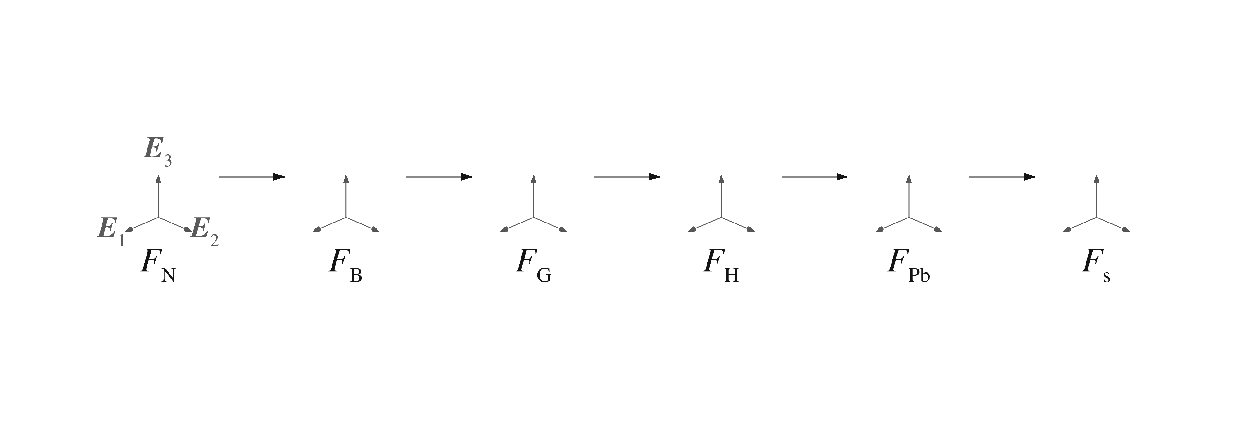
\includegraphics[width=.96\linewidth,height=.40\textheight,keepaspectratio]{figures/tecplot/concept_arbol.pdf}
\caption[Relaciones entre los sistemas de referencia]{Jerarquía de los sistemas de referencia: newtoniano $N$, base $B$, góndola $G$, cubo $H$, raíz $P_b$ y sección $s$. Cada símbolo $\mathcal F$ identifica un triedro espacial. Las flechas indican relaciones cinemáticas y cambios de componentes; las ubicaciones son esquemáticas y no imponen conexiones rígidas.}\label{fig:arbol}
\end{figure}

\subsection{Construcción explícita de las posiciones de los componentes}
Los sistemas de referencia anteriores permiten escribir posiciones sin ambigüedad. Para una partícula de la torre, con $\vct R_T(S)=S\vct E_3$ en la referencia recta, se usa
\begin{equation}
 \vct x_T=\vct c_B(t)+\vct R_T(S)+\vct u_T(S,t)
 +\xi_2\vct d_{2T}(S,t)+\xi_3\vct d_{3T}(S,t).
\end{equation}
Aquí $\vct u_T$ es el desplazamiento de la línea de torre relativo a la base. La traslación sísmica $\vct u_B$ aparece una sola vez, en $\vct c_B$. Para una góndola rígida,
\begin{equation}
 \vct x_G=\vct c_G(t)+{}^NQ_G(t)\vct\rho_G,
\end{equation}
donde $\vct\rho_G$ identifica una partícula respecto del punto de referencia elegido en el cuerpo. Si la góndola está soldada a la sección superior de torre, $\vct c_G$ y ${}^NQ_G$ se deducen de esa sección y de la separación geométrica de montaje. Si existe una unión flexible, la diferencia relativa constituye una incógnita y la unión aporta una relación constitutiva entre acciones y desplazamientos relativos, no una identidad cinemática.

Para el cubo--nariz rígido se escribe análogamente
\begin{equation}
 \vct x_H=\vct c_H(t)+{}^NQ_H(t)\vct\rho_H,
 \qquad {}^NQ_H={}^N\overline Q_H\exp([\vct\theta_H]_\times).
\end{equation}
El vector $\vct\rho_H$ permanece fijo en el cuerpo; $\vct\theta_H$ es una perturbación respecto del giro nominal. Se distingue de $\psi$, que puede recorrer muchas revoluciones. La nariz comparte esta expresión solamente bajo la idealización rígida conjunta declarada.

Una pala se describe en su propio sistema de referencia de raíz: $\vct r_b^P(S,t)$ es la posición de su línea respecto a la raíz y $\vct d_{\alpha b}^P$ son sus directores. La posición absoluta de una partícula resulta
\begin{equation}
 \vct x_b=\vct c_{P_b}(t)+{}^NQ_{P_b}(t)
 \left[\vct r_b^P(S,t)+\xi_2\vct d_{2b}^P+\xi_3\vct d_{3b}^P\right].
\end{equation}
En una raíz soldada, $\vct c_{P_b}=\vct c_H+{}^NQ_H\vct r_{b0}^H$ y ${}^NQ_{P_b}={}^NQ_H{}^HQ_{P_b}$, con $\vct r_{b0}^H$ fijo. Entonces se elige $\vct r_b^P(0,t)=0$ y la orientación relativa de raíz coincide con el montaje. La deformación de las secciones interiores sigue siendo libre. Estas expresiones describen campos continuos; imponer su versión nodal corresponde al capítulo de elementos finitos.

La figura~\ref{fig:cadena-posiciones} representa la suma de posiciones de la ecuación anterior, desde el origen newtoniano hasta la partícula de pala.

\begin{figure}[htbp]
\centering
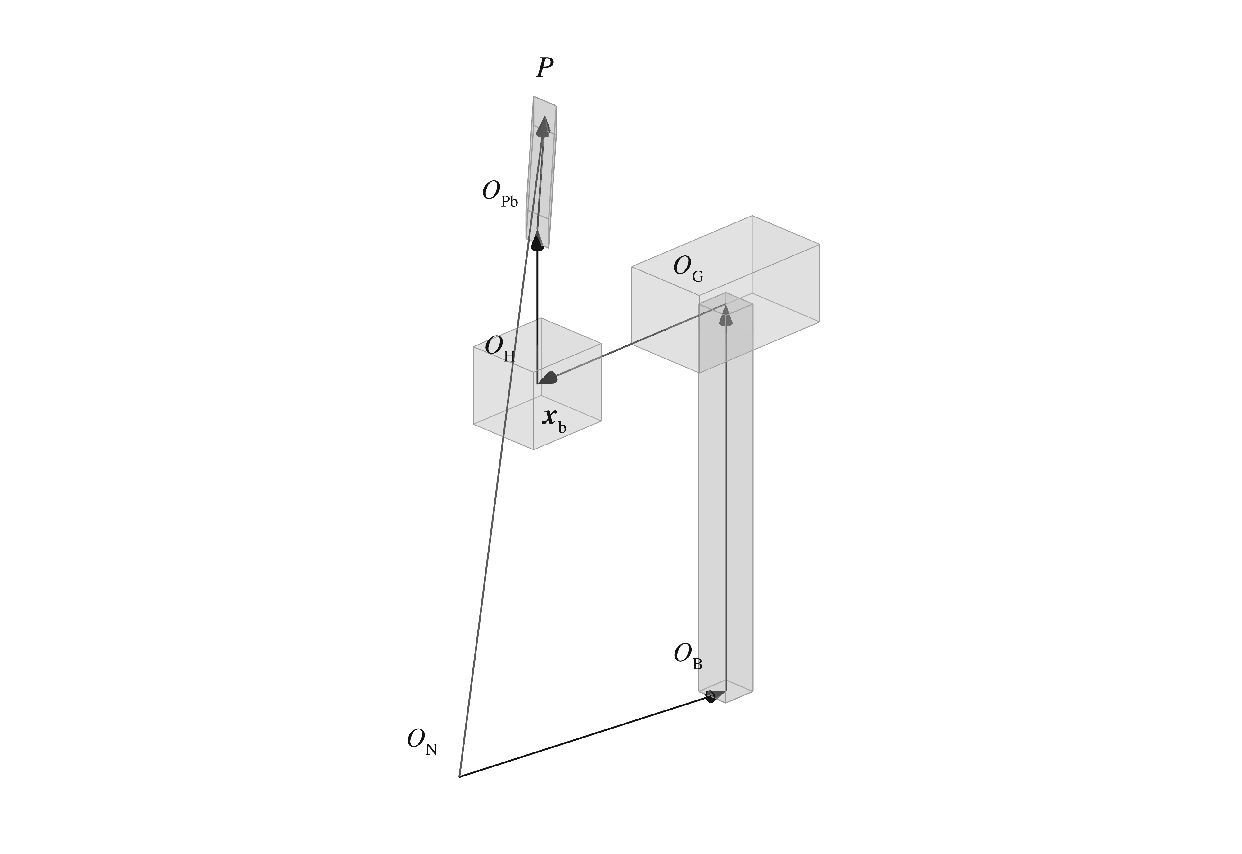
\includegraphics[width=.96\linewidth,height=.40\textheight,keepaspectratio]{figures/tecplot/concept_cadena-posiciones.pdf}
\caption[Composición de posiciones]{Composición de posiciones desde el origen newtoniano hasta una partícula de pala. Los puntos intermedios corresponden a la base, la góndola, el cubo y la raíz. La flecha directa representa la posición absoluta $\vct x_b$. El esquema espacial no está a escala.}\label{fig:cadena-posiciones}
\end{figure}

\section{Movimiento nominal y configuración deformada}
\subsection{Configuración de referencia, movimiento nominal y configuración actual}
Para una partícula del rotor puede definirse un movimiento nominal rígido
\begin{equation}
 \overline{\vct\chi}(\vct X,t)=\overline{\vct c}_H(t)
 +{}^N\overline Q_H(t)\vct a(\vct X),
\end{equation}
donde $\vct a$ es su posición material relativa al cubo en coordenadas nominales. Si se añaden deformaciones, el movimiento actual será
\begin{equation}
 \vct\chi(\vct X,t)=\overline{\vct c}_H(t)+{}^N\overline Q_H(t)
 [\vct a(\vct X)+\vct u_c(\vct X,t)].
 \label{eq:nominalactual}
\end{equation}
El subíndice $c$ indica componentes en el sistema de referencia nominal corrotante, no que el material permanezca rígido. La deformación operativa, por ejemplo debida a las cargas medias, puede incluirse en $\vct u_c=\vct u_{c0}+\widetilde{\vct u}_c$. La tilde denota una perturbación alrededor de esa deformación operativa.

La configuración de referencia identifica las partículas mediante sus coordenadas materiales. El movimiento nominal describe la traslación y la rotación prescritas de esa geometría. El estado de operación incorpora las deformaciones asociadas a las cargas y al giro, y la configuración actual contiene además la perturbación vibratoria. Estas definiciones permiten describir una misma partícula desde la geometría inicial hasta su posición durante la operación.

En la figura~\ref{fig:tresniveles}, $\overline{\mathcal B}_t$ denota la configuración ocupada bajo el movimiento nominal y $\overline{\vct x}=\overline{\vct\chi}(\vct X,t)$. La diferencia de posiciones se expresa en ejes inerciales: $\vct x-\overline{\vct x}={}^N\overline Q_H\vct u_c$. La traslación nominal del cubo aparece en ambas posiciones y se cancela en esa diferencia.
\begin{figure}[htbp]
\centering
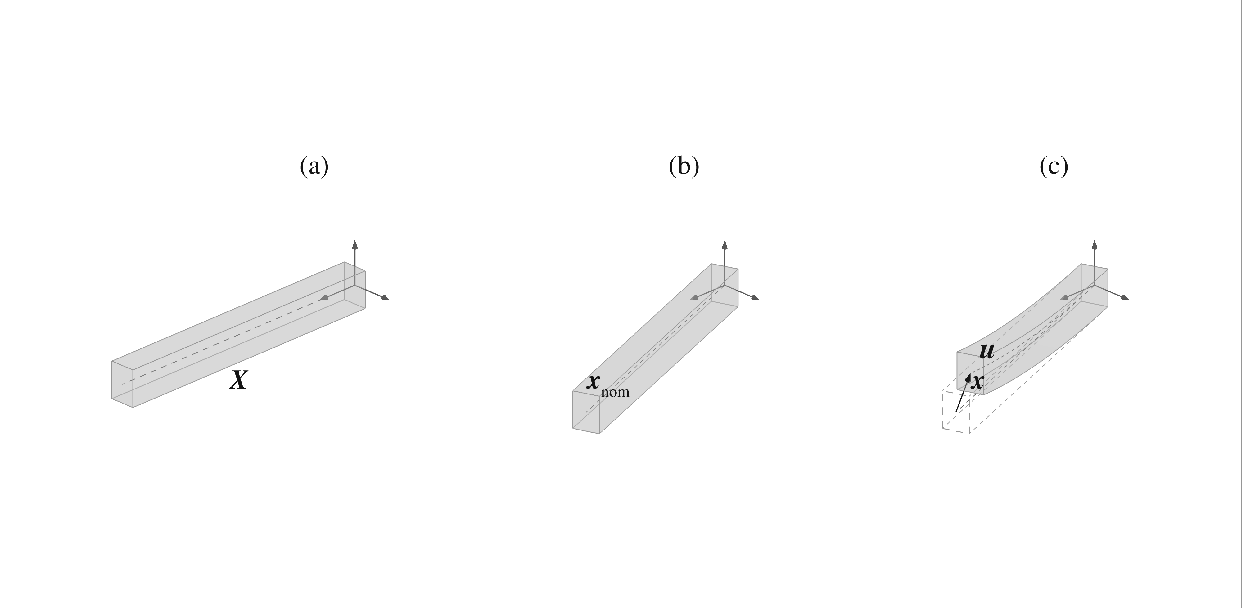
\includegraphics[width=.96\linewidth,height=.40\textheight,keepaspectratio]{figures/tecplot/concept_tresniveles.pdf}
\caption[Referencia material, movimiento nominal y perturbación]{Una misma porción de viga en (a) referencia material, (b) movimiento nominal y (c) configuración actual. El contorno discontinuo de (c) reproduce la configuración nominal; la diferencia se identifica mediante $\vct u$. Los pequeños triedros conservan la orientación inercial en los tres paneles.}\label{fig:tresniveles}
\end{figure}

\subsection{Giro prescrito y grados de libertad estructurales}
Al suprimir las deformaciones del rotor, su movimiento nominal se describe por un solo parámetro angular. Como $\psi(t)$ está dado, ese parámetro no se cuenta entre las incógnitas dinámicas. La turbina completa no se convierte en un sólido de un grado de libertad: permanecen la torre estacionaria, las conexiones y, cuando se restituyen, las múltiples perturbaciones estructurales.

Una perturbación torsional del eje representa una desviación respecto del giro prescrito. Si se incluye y existe rigidez torsional, no es un mecanismo libre. Si se elimina por una restricción de velocidad ideal, no debe aparecer como incógnita adicional. La elección depende de la representación del tren de potencia y debe declararse antes del análisis modal.

\section{Cinemática continua de una viga espacial}
\subsection{Línea de referencia y directores}
Se parametriza la viga por una coordenada material $S\in[0,L]$ y dos coordenadas transversales $\xi_2,\xi_3$. En referencia,
\begin{equation}
 \vct X(S,\xi_2,\xi_3)=\vct R(S)+\xi_2\vct D_2(S)+\xi_3\vct D_3(S).
\end{equation}
La línea $\vct R(S)$ une los puntos de referencia de las secciones. Los directores $\vct D_i$ son unitarios y ortogonales, con $\vct D_1=\vct D_2\times\vct D_3$. En la configuración actual, bajo la hipótesis de sección rígida,
\begin{equation}
 \vct x(S,\xi_2,\xi_3,t)=\vct r(S,t)+\xi_2\vct d_2(S,t)+\xi_3\vct d_3(S,t).
 \label{eq:beamkin}
\end{equation}
La misma partícula conserva $S,\xi_2,\xi_3$. La hipótesis excluye deformación dentro del plano de la sección y alabeo explícito, pero admite su traslación y orientación independientes. El efecto del alabeo de torsión puede incorporarse en una rigidez seccional efectiva sin resolverlo como campo cinemático adicional.

El punto $\vct r(S,t)$ es el origen elegido para una sección, no necesariamente su centro de masa ni su centro geométrico. Los directores $\vct d_2$ y $\vct d_3$ indican las direcciones de las coordenadas transversales. El director $\vct d_1=\vct d_2\times\vct d_3$ completa la base ortonormal y es normal a la sección. La posición de una partícula se reconstruye sumando la posición del origen seccional y los dos vectores transversales. De esta manera, las tres coordenadas materiales identifican una partícula del volumen, mientras que los campos $\vct r$ y $Q$ describen el movimiento de toda la viga.

La figura~\ref{fig:particula-seccion} separa la posición del origen seccional de la posición de la partícula dentro de esa sección.

\begin{figure}[htbp]
\centering
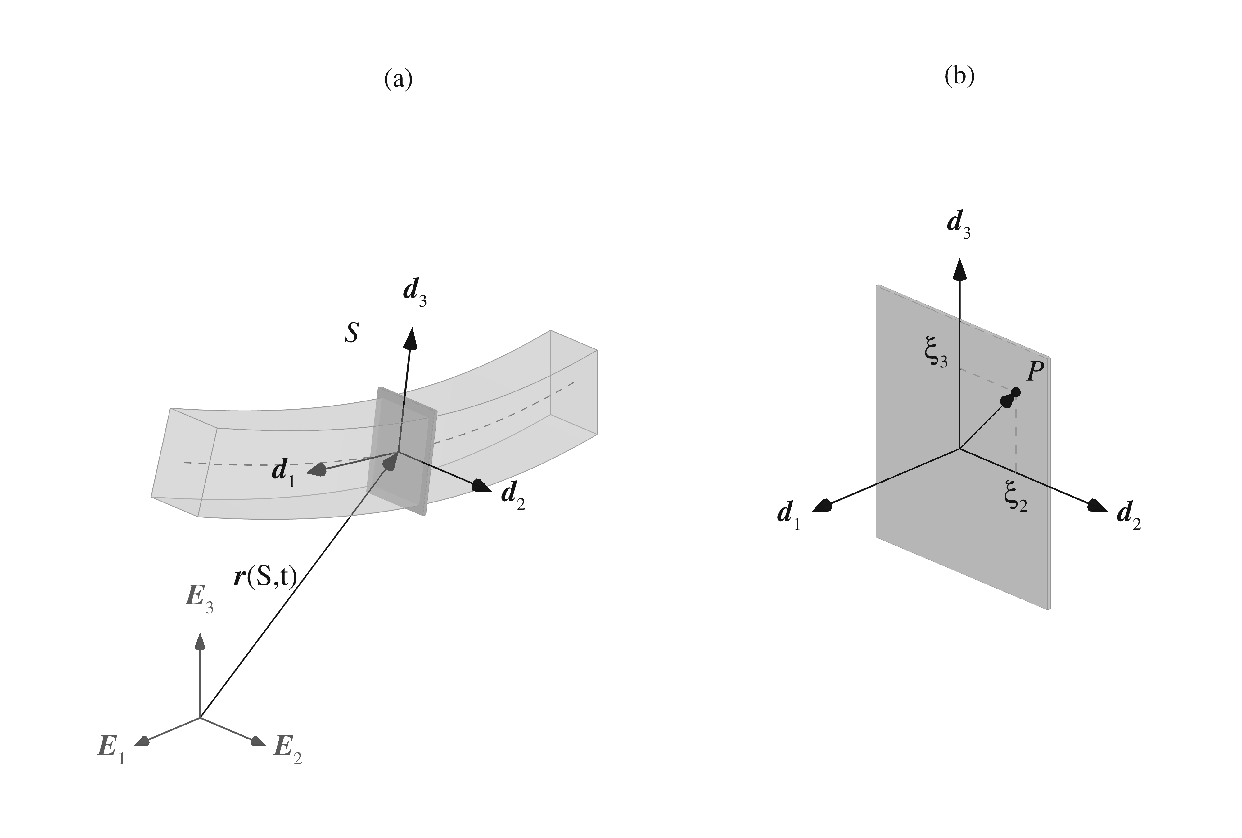
\includegraphics[width=.96\linewidth,height=.40\textheight,keepaspectratio]{figures/tecplot/concept_particula-seccion.pdf}
\caption[Posición de una partícula de viga]{Posición de una partícula de viga. (a) Línea de referencia $\vct r(S,t)$, sección rígida y triedro de directores. (b) Ampliación de la sección: $\vct x_P=\vct r+\xi_2\vct d_2+\xi_3\vct d_3$. Se muestran los tres directores; $\vct d_1$ es normal a la sección. El volumen transparente representa la envolvente de la viga.}\label{fig:particula-seccion}
\end{figure}

Sean $Q_0=[\vct D_1,\vct D_2,\vct D_3]$ y $Q=[\vct d_1,\vct d_2,\vct d_3]$ en componentes newtonianas. Ambas matrices pertenecen a $\SO$. La rotación física que lleva los directores iniciales a los actuales es $QQ_0^\tr$.

\subsection{Extensión y cortante}
Con prima indicando derivada respecto de $S$, se define
\begin{equation}
 \vct\gamma=Q^\tr\vct r'-Q_0^\tr\vct R'.
 \label{eq:gamma}
\end{equation}
Esta terna expresa el cambio del vector tangente medido por la propia sección. Si $S$ es longitud de arco de referencia y $\vct R'=\vct D_1$, el segundo término es $(1,0,0)^\tr$. La componente $\gamma_1$ representa extensión de la línea, mientras $\gamma_2$ y $\gamma_3$ describen cortante. El director $\vct d_1$ no se impone paralelo a $\vct r'$. Imponerlo anularía el cortante y cambiaría la teoría de viga.

La figura~\ref{fig:shear} muestra la diferencia entre la normal a la sección y la tangente a la línea deformada, que da lugar a la deformación por cortante.

\begin{figure}[htbp]
\centering
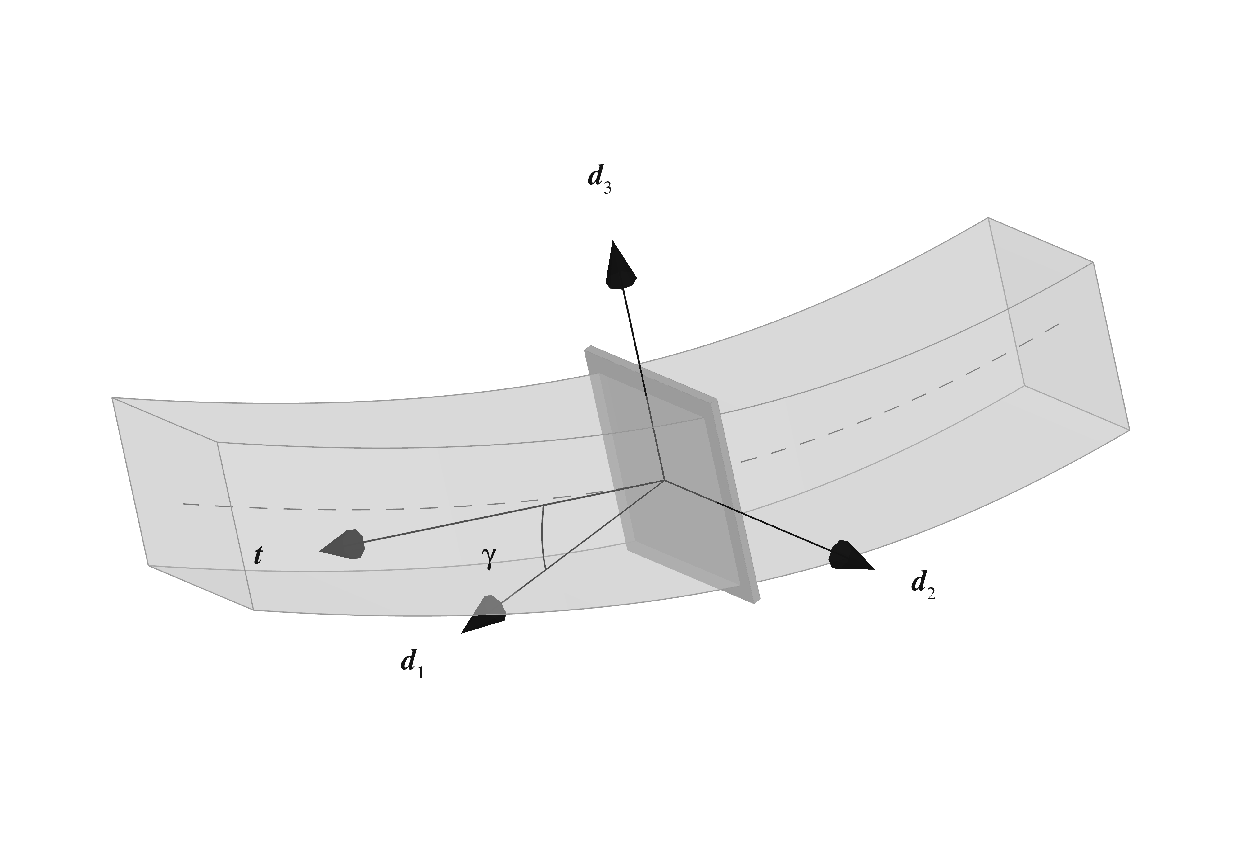
\includegraphics[width=.96\linewidth,height=.40\textheight,keepaspectratio]{figures/tecplot/concept_shear.pdf}
\caption[Normal a la sección y tangente a la línea]{Normal $\vct d_1$ a la sección y tangente $\vct t$ a la línea de referencia de una viga con cortante. El arco $\gamma$ mide el ángulo entre ambas direcciones en el esquema espacial. La rigidez de la sección no obliga a que su normal coincida con la tangente.}\label{fig:shear}
\end{figure}

\subsection{Curvatura y torsión}
Como $Q^\tr Q=\Id$, la matriz $Q^\tr Q'$ es antisimétrica. Se define
\begin{equation}
 \vct\kappa=\ax(Q^\tr Q')-\ax(Q_0^\tr Q_0').
 \label{eq:kappa}
\end{equation}
Su primera componente mide torsión y las otras dos flexión. Se resta la curvatura material inicial para que una geometría precurvada sin deformación no produzca curvatura elástica. Las componentes se interpretan con respecto a las mismas etiquetas materiales de los directores.

Estas medidas son objetivas ante una traslación y rotación rígida superpuestas: si $\vct r^*=\vct c+P\vct r$, $Q^*=PQ$ y $P$ no depende de $S$, entonces $(Q^*)^\tr(\vct r^*)'=Q^\tr\vct r'$ y $(Q^*)^\tr(Q^*)'=Q^\tr Q'$. Un movimiento rígido no cambia $\vct\gamma$ ni $\vct\kappa$. Esta invariancia permite conservar el giro nominal sin atribuirle deformaciones espurias.

\subsection{Relación con el gradiente tridimensional}
La reducción de viga puede conectarse con $\ten F$ sin introducir nodos. Definiendo
\begin{align}
 \vct G_1&=\vct R'+\xi_2\vct D_2'+\xi_3\vct D_3',&
 \vct G_2&=\vct D_2,&\vct G_3&=\vct D_3,\\
 \vct g_1&=\vct r'+\xi_2\vct d_2'+\xi_3\vct d_3',&
 \vct g_2&=\vct d_2,&\vct g_3&=\vct d_3,
\end{align}
y la base recíproca $\vct G^i\cdot\vct G_j=\delta^i_j$, se obtiene $\ten F=\vct g_i\otimes\vct G^i$. La necesidad de base recíproca explica por qué no se puede tratar sin más una parametrización curva como cartesiana. El modelo unidimensional conserva ciertas deformaciones del continuo y elimina otras por hipótesis.

\section{Rotaciones finitas y perturbaciones pequeñas}
\subsection{Representación exponencial}
La orientación perturbada de un triedro nominal $\overline Q$ se escribe
\begin{equation}
 Q=\overline Q E(\vct\theta),\qquad E(\vct\theta)=\exp(\sk\theta).
 \label{eq:exprot}
\end{equation}
Las componentes de $\vct\theta$ están en la base nominal que precede a $E$. Para $\vartheta=\|\vct\theta\|$, la fórmula de Rodrigues es
\begin{equation}
 E=\Id+\frac{\sin\vartheta}{\vartheta}\sk\theta
 +\frac{1-\cos\vartheta}{\vartheta^2}\sk\theta^2,
\end{equation}
con límites continuos en cero. El vector de rotación es una parametrización local; no es una terna de ángulos de Euler. Dos rotaciones finitas se componen multiplicando sus matrices, no sumando sus vectores. A primer orden, $E\simeq\Id+\sk\theta$, y solo en ese régimen las sumas de pequeños incrementos son compatibles con una aproximación lineal.

En la figura~\ref{fig:giro-perturbacion} se presenta un caso particular que permite separar visualmente las dos rotaciones: tanto el giro nominal como la perturbación se toman alrededor del eje 1. En ese caso especial sus ángulos pueden sumarse. Para una perturbación general, sus tres componentes se incorporan mediante el producto matricial~\eqref{eq:exprot}; el dibujo no justifica sumar ángulos alrededor de ejes diferentes.

\begin{figure}[htbp]
\centering
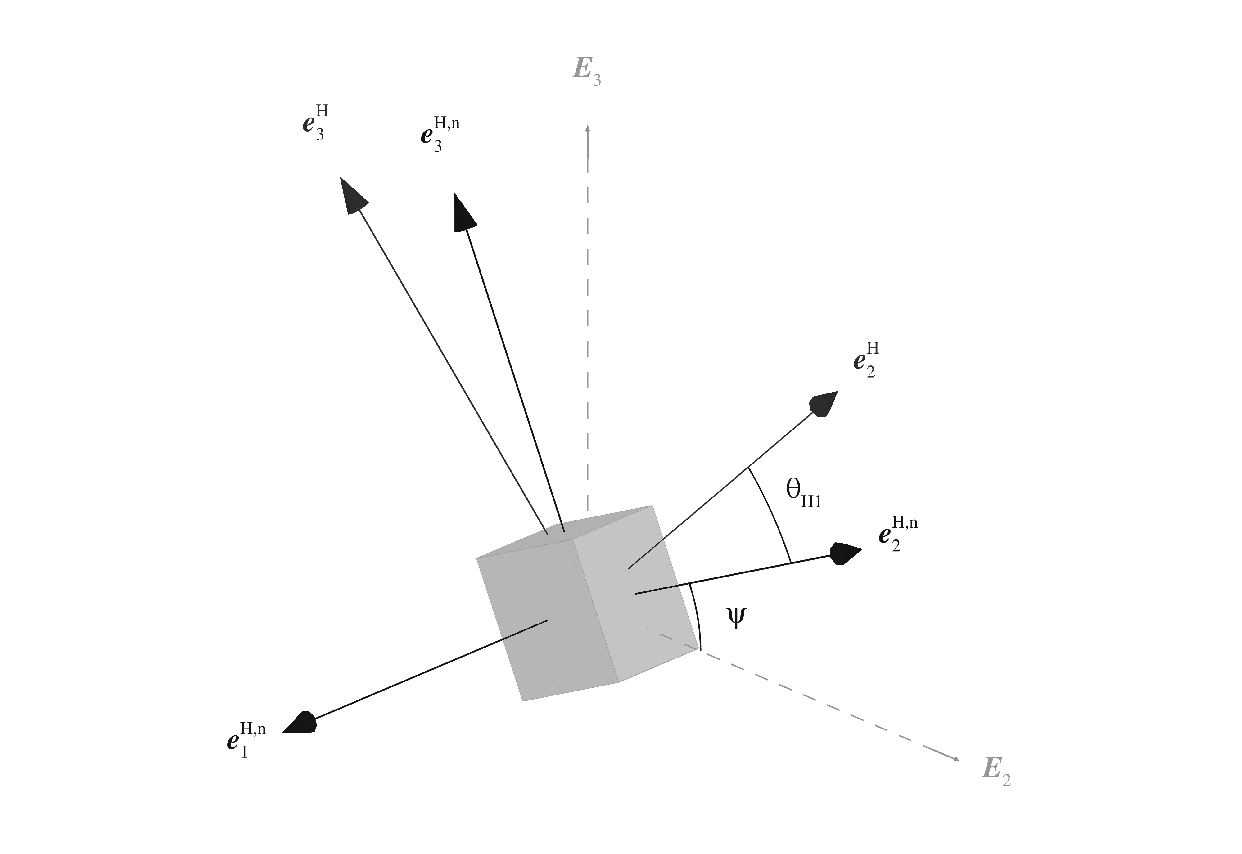
\includegraphics[width=.96\linewidth,height=.40\textheight,keepaspectratio]{figures/tecplot/concept_giro-perturbacion.pdf}
\caption[Rotación nominal y perturbación angular]{Separación de la orientación inercial, la rotación nominal $\psi$ y una perturbación rotacional del cubo. El superíndice $H,n$ indica la base nominal y $H$ la perturbada. El incremento $\theta_{H1}$ se amplía para distinguir los triedros; la formulación emplea pequeñas perturbaciones.}\label{fig:giro-perturbacion}
\end{figure}

\subsection{Velocidad angular y derivada del vector de rotación}
En general $\dot{\vct\theta}$ no es la velocidad angular exacta. La identidad
\begin{equation}
 \dot E E^\tr=\sk{J_\ell(\vct\theta)\dot{\vct\theta}},\quad
 J_\ell(\vct\theta)=\Id+
 \frac{1-\cos\vartheta}{\vartheta^2}\sk\theta+
 \frac{\vartheta-\sin\vartheta}{\vartheta^3}\sk\theta^2
\end{equation}
define el Jacobiano izquierdo de la parametrización exponencial. En particular,
\begin{equation}
 J_\ell\dot{\vct\theta}=\dot{\vct\theta}
 +\tfrac12\vct\theta\times\dot{\vct\theta}+O(\epsilon^3)
\end{equation}
si $\vct\theta$ y su derivada son de orden $\epsilon$. El término cuadrático puede contribuir a las ecuaciones lineales al multiplicarse por una velocidad nominal no nula en la energía cinética. Por ello no siempre es correcto linealizar todas las velocidades antes de formar la energía que se va a expandir.

\subsection{Límite de pequeñas deformaciones de una viga recta}
Para una viga inicialmente recta en el eje local 1, con $Q_0=\Id$, se toma $\vct r=(S,0,0)^\tr+\vct u$ y $Q\simeq\Id+\sk\theta$. Al retener primer orden,
\begin{equation}
 \vct\gamma=\vct u'-\vct\theta\times\vct e_1,
 \qquad \vct\kappa=\vct\theta'.
\end{equation}
Como $\vct\theta\times\vct e_1=(0,\theta_3,-\theta_2)^\tr$, se obtiene
\begin{equation}
 \vct e_s=
 [u_1',\ u_2'-\theta_3,\ u_3'+\theta_2,\ \theta_1',\ \theta_2',\ \theta_3']^\tr.
 \label{eq:strainlinear}
\end{equation}
Esta expresión fija los signos que se emplearán al construir la matriz deformación--desplazamiento. Aún no hay nodos: $\vct u(S,t)$ y $\vct\theta(S,t)$ son campos continuos.

\section{Velocidades y aceleraciones en el sistema giratorio}
\subsection{Posición y velocidad de una partícula}
Sea $Q_c(t)={}^N\overline Q_H(t)$ y $\vct y(t)$ la posición relativa de una partícula en ese sistema de referencia. Definimos $\vct\Omega_c=\Omega\vct e_1$ y $W=\sk{\Omega_c}$, de manera que $\dot Q_c=Q_cW$. La posición y velocidad absolutas son
\begin{align}
 \vct x&=\vct c(t)+Q_c(t)\vct y(t),\\
 \dot{\vct x}&=\dot{\vct c}+Q_c(\dot{\vct y}+W\vct y).
 \label{eq:velocitytransport}
\end{align}
El término $Q_c\dot{\vct y}$ es velocidad relativa transportada a la base newtoniana. El término $Q_cW\vct y$ existe aunque la partícula esté fija en el sistema de referencia giratorio. La suma se realiza después de expresar ambos en una base común.

La suma de la ecuación~\eqref{eq:velocitytransport} se representa en la figura~\ref{fig:suma-velocidades}. No se suman velocidades medidas por observadores diferentes sin transformar sus componentes. Cada lado del polígono es ya una velocidad expresada en el sistema newtoniano.

\begin{figure}[htbp]
\centering
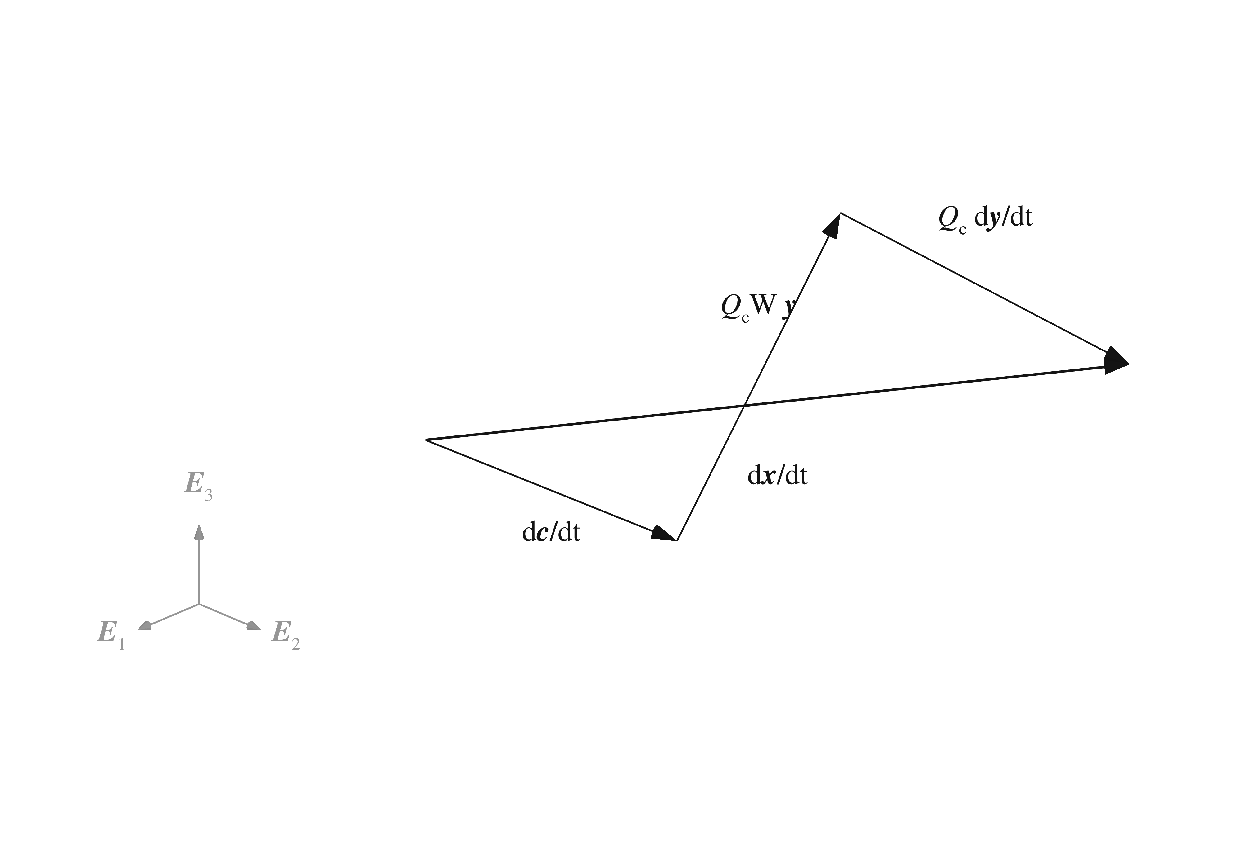
\includegraphics[width=.96\linewidth,height=.40\textheight,keepaspectratio]{figures/tecplot/concept_suma-velocidades.pdf}
\caption[Composición de velocidades]{Suma vectorial de los tres términos del teorema de transporte. Las flechas sucesivas representan la velocidad de traslación del origen, la contribución de la rotación de la base y la velocidad relativa transformada. La flecha directa cierra la suma y representa $\dd\vct x/\dd t$. Todas las contribuciones están expresadas en una base común.}\label{fig:suma-velocidades}
\end{figure}

\subsection{Aceleración y origen de los términos de giro}
Derivando de nuevo, con posibilidad inicial de $W=W(t)$,
\begin{equation}
 \ddot{\vct x}=\ddot{\vct c}
 +Q_c\left[\ddot{\vct y}+2W\dot{\vct y}
 +\dot W\vct y+W^2\vct y\right].
 \label{eq:acceltransport}
\end{equation}
La aceleración consta de cinco contribuciones: traslación del origen, aceleración relativa, transporte de Coriolis, aceleración asociada a variación de la velocidad angular y aceleración normal del giro. En la operación prescrita de eje fijo y velocidad constante, $\dot W=0$. No se elimina $2W\dot{\vct y}$: las perturbaciones pueden tener velocidad relativa aunque $\Omega$ sea constante.

La identidad $W^2\vct y=\vct\Omega_c(\vct\Omega_c\cdot\vct y)-\Omega^2\vct y$ muestra que este término apunta hacia el eje en la componente transversal. Se denomina \emph{aceleración centrípeta nominal}. Al trasladarlo al lado de las acciones en una ecuación escrita en sistema de referencia giratorio aparece con signo contrario. No son dos interacciones físicas independientes que deban sumarse.

La figura~\ref{fig:centripeta} identifica las direcciones tangencial y radial de estas contribuciones cinemáticas en el plano del rotor.

\begin{figure}[htbp]
\centering
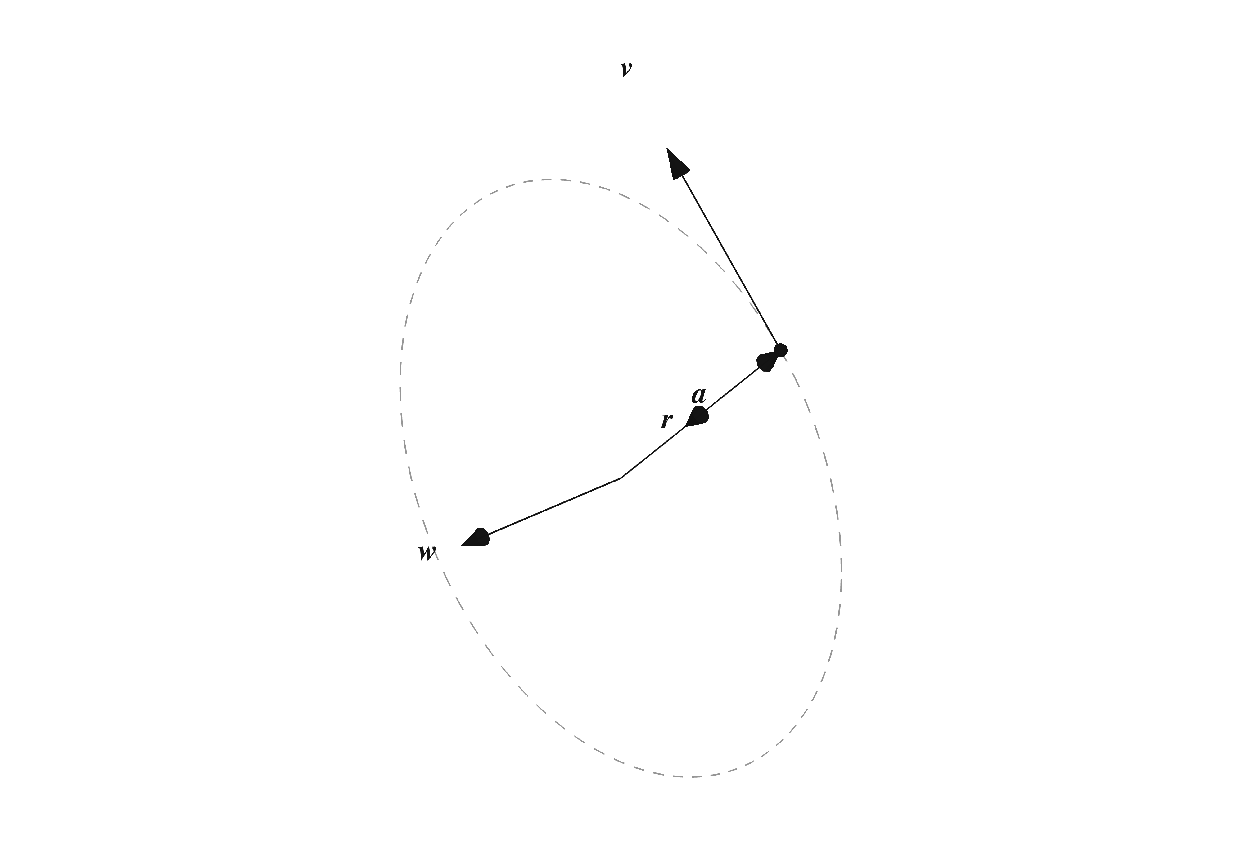
\includegraphics[width=.96\linewidth,height=.40\textheight,keepaspectratio]{figures/tecplot/concept_centripeta.pdf}
\caption[Velocidad y aceleración nominales]{Movimiento circular de un punto fijo en la base nominal del rotor. La velocidad $\vct v$ es tangente a la trayectoria y perpendicular al radio $\vct r$; la aceleración centrípeta $\vct a$ apunta hacia el eje de giro. La flecha axial indica la dirección de la velocidad angular.}\label{fig:centripeta}
\end{figure}

\subsection{Centro de masa excéntrico de una sección}
Para relacionar la cinemática con la inercia, sean $\vct a$ la posición nominal del punto de referencia de una sección respecto del cubo y $\vct c_m$ el vector que une ese punto con el centro de masa seccional. Se expresan ambos en una misma base nominal. Con traslación perturbada $\vct u$ y rotación $E$,
\begin{equation}
 \vct y_C=\vct a+\vct u+E\vct c_m,
 \qquad \vct x_C=\vct c+Q_c\vct y_C.
\end{equation}
Así,
\begin{equation}
 {}^c\vct v_C=Q_c^\tr\dot{\vct c}+W\vct y_C+\dot{\vct u}
 +\left[J_\ell(\vct\theta)\dot{\vct\theta}\right]_\times E\vct c_m,
 \label{eq:vgfull}
\end{equation}
y la velocidad angular total en componentes nominales es
\begin{equation}
 {}^c\vct\omega=\vct\Omega_c+J_\ell(\vct\theta)\dot{\vct\theta}.
\end{equation}
Si una propiedad se conoce inicialmente en la base de pala, se lleva antes a la base nominal elegida mediante su matriz de montaje. No se multiplica un tensor expresado en ejes de pala por una velocidad angular expresada en ejes de cubo sin ese cambio. Esta precaución es esencial para los efectos giroscópicos y los productos de inercia.

\section{Equilibrio de operación y movimiento síncrono}
\subsection{Estacionariedad relativa}
Una deformación constante vista desde el rotor puede seguir moviéndose respecto de $N$. Si $\vct u_c=\vct u_{c0}$ y $\vct\theta=\vct\theta_0$ son constantes, las partículas siguen trayectorias por $Q_c(t)$ aunque sus coordenadas relativas no cambien. Se habla de equilibrio relativo cuando esa configuración satisface las ecuaciones de movimiento en el sistema de referencia apropiado, no solo porque las coordenadas se mantengan constantes por definición.

La configuración de equilibrio de operación depende de velocidad, cargas y condiciones de apoyo. En ausencia de invariancia de las cargas respecto del giro, una deformación constante corrotante puede no existir. Por ejemplo, la gravedad es fija en $N$, pero sus componentes en el rotor cambian con el azimut. El cortante vertical de viento produce también una excitación periódica durante el paso de las palas.

La figura~\ref{fig:gravedad-giratoria} muestra esta diferencia con una magnitud conocida. Para la góndola horizontal y $\vct g=-g\vct E_3$, sus componentes en la base nominal del cubo son
\begin{equation}
 {}^H\vct g=({}^N\overline Q_H)^\tr(-g\vct E_3)
 =\begin{bmatrix}0\\-g\sin\psi\\-g\cos\psi\end{bmatrix}.
\end{equation}
La variación de esas componentes no significa que cambie la gravedad física. Significa que la misma dirección espacial se observa desde ejes que giran. Una operación uniforme puede, por tanto, coexistir con excitaciones periódicas en las coordenadas del rotor.

\begin{figure}[htbp]
\centering
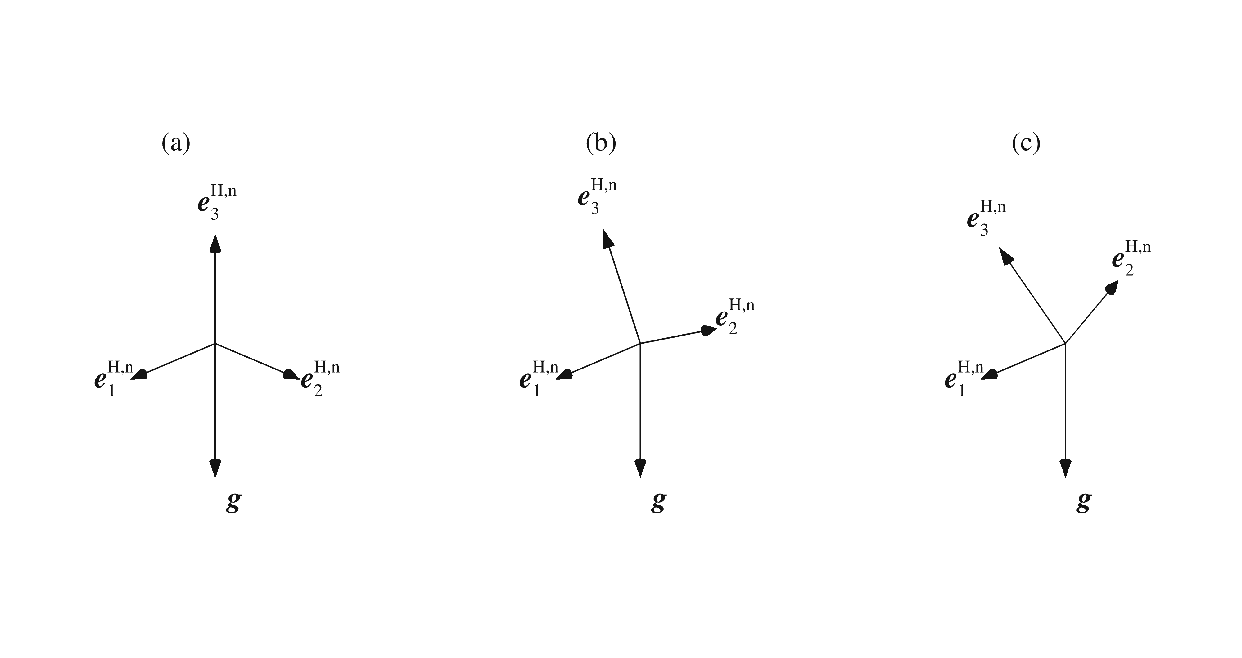
\includegraphics[width=.96\linewidth,height=.40\textheight,keepaspectratio]{figures/tecplot/concept_gravedad-giratoria.pdf}
\caption[Gravedad expresada en ejes giratorios]{La misma gravedad inercial $\vct g$ observada con tres orientaciones nominales del cubo. El vector geométrico conserva su dirección, pero sus componentes en la base $H,n$ varían con el azimut. Los paneles presentan ángulos ilustrativos.}\label{fig:gravedad-giratoria}
\end{figure}

\subsection{Estado a azimut fijo y solución periódica}
El equilibrio local calculado para un azimut $\psi_*$ no demuestra una solución periódica completa. En el primer caso se resuelve una ecuación residual algebraica con parámetros fijados; en el segundo, la trayectoria debe satisfacer las ecuaciones durante todo el período $T=2\pi/\Omega$, además de la condición de periodicidad. El término \emph{movimiento síncrono} se reserva para una respuesta ligada a la fase de giro, por ejemplo una respuesta periódica de período $T$. No toda vibración tiene que ser síncrona.

La figura~\ref{fig:operacion} ilustra la separación entre una coordenada de equilibrio constante y su perturbación vibratoria; no representa una respuesta numérica del aerogenerador.

\begin{figure}[htbp]
\centering
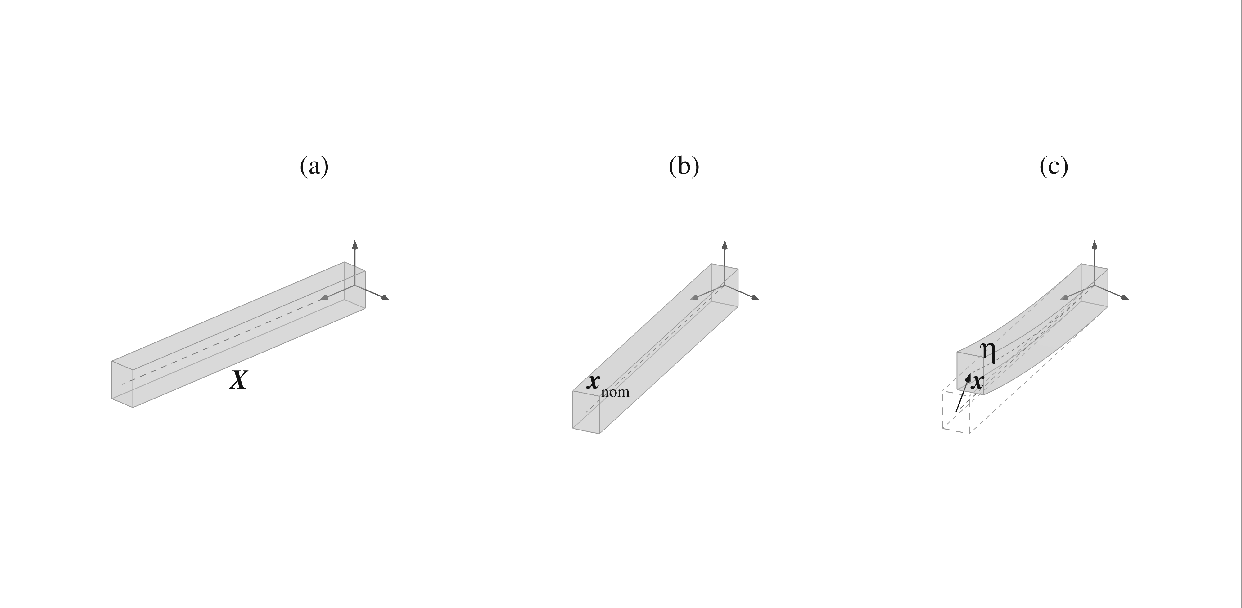
\includegraphics[width=.96\linewidth,height=.40\textheight,keepaspectratio]{figures/tecplot/concept_operacion.pdf}
\caption[Equilibrio y perturbación]{Separación geométrica entre referencia, configuración nominal y configuración actual con perturbación $\vct\eta$. El contorno discontinuo en (c) permite comparar el estado nominal con el actual. La figura ilustra una separación cinemática y no es una solución calculada de equilibrio ni una historia temporal.}\label{fig:operacion}
\end{figure}

\subsection{Vínculo con los modos de vibración}
Después de discretizar, el vector $\vct q_0$ representará las coordenadas del equilibrio, mientras $\vct\phi_j$ representará una dirección de perturbación modal. Son objetos diferentes. La relación es que las matrices linealizadas se evalúan alrededor de $\vct q_0$ y, por tanto, los modos dependen de él. No se obtiene $\vct q_0$ resolviendo el problema homogéneo de autovalores. El capítulo~\ref{ch:operacion} establece esta conexión y el caso particular en que una deformación estática admite una expansión en modos.

Las posiciones, orientaciones y velocidades definidas en este capítulo permiten calcular el movimiento de cualquier partícula de la torre, las palas y los cuerpos rígidos. Las medidas de deformación caracterizan la variación relativa entre secciones, mientras que el transporte temporal incorpora la rotación nominal. Las propiedades de masa y rigidez relacionan ahora estos campos cinemáticos con la energía cinética, la cantidad de movimiento y las fuerzas internas.

\chapter{Propiedades geométricas, de masa y de rigidez}
\label{ch:propiedades}
\section{Geometría, densidad y medida de integración}
Una propiedad másica no se identifica únicamente por su valor: debe conocerse el dominio sobre el que se integra, el punto respecto del cual se calcula y la base utilizada para sus componentes. En una viga, las propiedades por unidad de longitud se definen sobre la sección material de referencia $A_0(S)$. Para una sección recta se usa el vector transversal $\vct\zeta=\xi_2\vct D_2+\xi_3\vct D_3$. La densidad de referencia $\rho_0$ se mide en $\mathrm{kg/m^3}$.

Se adopta localmente la medida prismática $\dd V_0=\dd A_0\dd S$, válida para el elemento recto empleado en la discretización. En una parametrización curva general, el determinante del transformación geométrica interviene en esta medida y no debe omitirse. La reducción a propiedades por longitud que sigue corresponde a esa aproximación local recta.

\section{Momentos geométricos de la sección}
El área, su primer momento y su centro geométrico son
\begin{equation}
 A=\int_{A_0}\dd A_0,\qquad
 \vct a_A=\int_{A_0}\vct\zeta\,\dd A_0,\qquad
 \vct c_A=\frac{\vct a_A}{A}.
\end{equation}
Con $\vct\eta_A=\vct\zeta-\vct c_A$, el tensor de segundos momentos geométricos se define por
\begin{equation}
 \ten S_A=\int_{A_0}\vct\eta_A\otimes\vct\eta_A\,\dd A_0,
 \qquad
 \ten I_A=\operatorname{tr}(\ten S_A)\Id-\ten S_A.
 \label{eq:area_tensor}
\end{equation}
Los tensores $\ten S_A$ e $\ten I_A$ tienen dimensión $\mathrm{m^4}$, son simétricos y describen la distribución de área, no de masa. El segundo es conveniente para relacionar un eje de giro con el segundo momento respecto a ese eje. En la base de sección con eje longitudinal $\vct D_1$, las coordenadas de $\vct\eta_A$ son $(0,y,z)$ y
\begin{equation}
 [\ten I_A]=
 \begin{bmatrix}
 \int(y^2+z^2)\dd A_0&0&0\\
 0&\int z^2\dd A_0&-\int yz\dd A_0\\
 0&-\int yz\dd A_0&\int y^2\dd A_0
 \end{bmatrix}.
\end{equation}
Así, $I_2=\int z^2\dd A_0$ e $I_3=\int y^2\dd A_0$. Un producto $\int yz\dd A_0$ no se introduce con signo positivo en las entradas fuera de la diagonal del tensor de inercia geométrico. Las direcciones principales diagonalizan su bloque transversal.

La constante torsional de Saint-Venant se denota $J_t$ y también tiene unidades de $\mathrm{m^4}$. No se identifica en general con $I_2+I_3$. Esta igualdad es válida para secciones circulares, pero no para una sección aerodinámica genérica: la distribución de tensiones de torsión depende del alabeo. Usar un momento polar de área como constante torsional sin esa justificación modifica la rigidez del modelo.

La figura~\ref{fig:centros} distingue el punto de referencia $O_s$, el centro de área $C_A$ y el centro de masa seccional $C_m$. Esta distinción permite definir a continuación las propiedades de masa sin suponer que los tres puntos coinciden.

\begin{figure}[htbp]
\centering
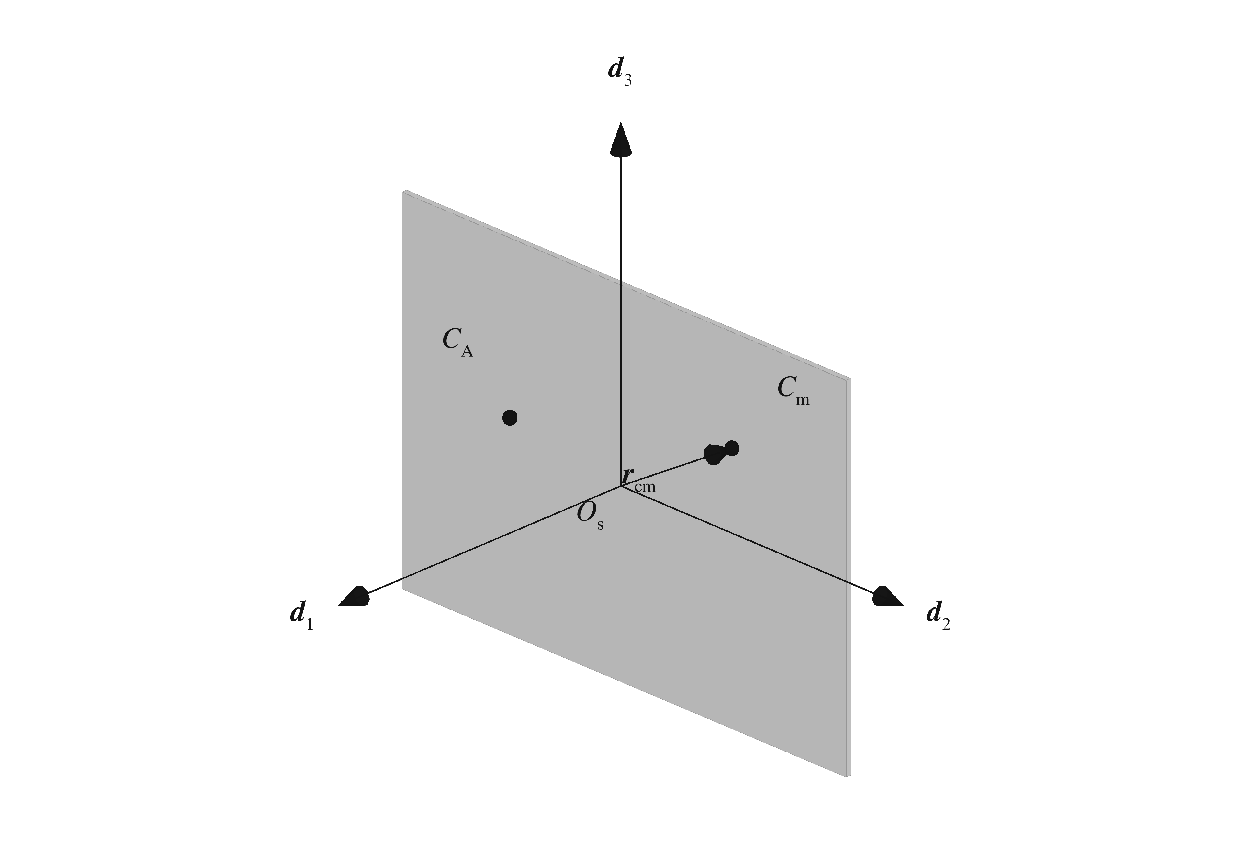
\includegraphics[width=.96\linewidth,height=.40\textheight,keepaspectratio]{figures/tecplot/concept_centros.pdf}
\caption[Punto de referencia y centros seccionales]{Sección con espesor ilustrativo y triedro completo: punto de referencia $O_s$, centro de área $C_A$ y centro de masa $C_m$. $\vct r_{cm}$ localiza el centro de masa respecto de $O_s$. Las posiciones se eligen para distinguir las definiciones; no corresponden a una sección medida.}\label{fig:centros}
\end{figure}

\section{Masa por longitud y tensor de inercia seccional}
La masa por longitud y el primer momento másico son
\begin{equation}
 \mu(S)=\int_{A_0}\rho_0\,\dd A_0,\qquad
 \vct h_m(S)=\int_{A_0}\rho_0\vct\zeta\,\dd A_0,\qquad
 \vct c_m=\frac{\vct h_m}{\mu}.
\end{equation}
El centro de masa depende de la densidad. Si esta es constante en la sección, $\vct c_m=\vct c_A$; una pala compuesta no cumple necesariamente esta condición. La inercia por longitud respecto de $C_m$, con $\vct\eta_m=\vct\zeta-\vct c_m$, es
\begin{equation}
 \ten j_C=\int_{A_0}\rho_0
 \left[(\vct\eta_m\cdot\vct\eta_m)\Id-\vct\eta_m\otimes\vct\eta_m\right]\dd A_0.
 \label{eq:jC}
\end{equation}
Sus unidades son $\mathrm{kg\,m}$, no $\mathrm{kg\,m^2}$. La integración posterior sobre $S$ incorpora la dimensión de longitud restante. Para cualquier vector angular $\vct\omega$,
\begin{equation}
 \vct\omega\cdot\ten j_C\vct\omega
 =\int_{A_0}\rho_0\|\vct\omega\times\vct\eta_m\|^2\dd A_0\geq0.
\end{equation}
Esta identidad muestra directamente su significado físico: cuantifica la energía cinética asociada al movimiento rotacional de la distribución de masa seccional.

En una sección plana, $j_1=j_2+j_3$ respecto del mismo centro y en una base ortonormal con eje 1 normal a la sección. No es una condición que se imponga a un cuerpo tridimensional arbitrario. Si $\rho_0$ es constante y los centros coinciden, $\ten j_C=\rho_0\ten I_A$.

El traslado al punto $O_s$ se deduce al introducir $\vct\zeta=\vct c_m+\vct\eta_m$ en la integral. Los términos lineales desaparecen porque $\int\rho_0\vct\eta_m\dd A_0=\vct0$. Resulta
\begin{equation}
 \ten j_O=\ten j_C+\mu\left[(\vct c_m\cdot\vct c_m)\Id-\vct c_m\otimes\vct c_m\right]
 =\ten j_C-\mu\sk{c_m}^{2}.
 \label{eq:steiner}
\end{equation}
El signo menos en la segunda forma no implica una disminución de inercia: $-\sk{c_m}^{2}$ es semidefinida positiva. Ambas expresiones son la misma identidad de ejes paralelos.

La figura~\ref{fig:masa-seccional} permite reconstruir la integral sin confundir los puntos de referencia. El vector material desde $O_s$ hasta una partícula es $\vct\zeta=\vct c_m+\vct\eta_m$. La integración respecto de $C_m$ utiliza $\vct\eta_m$; el traslado a $O_s$ utiliza la excentricidad $\vct c_m$. Por ello la identidad de ejes paralelos no sustituye al cambio de base del tensor.
\begin{figure}[htbp]
\centering
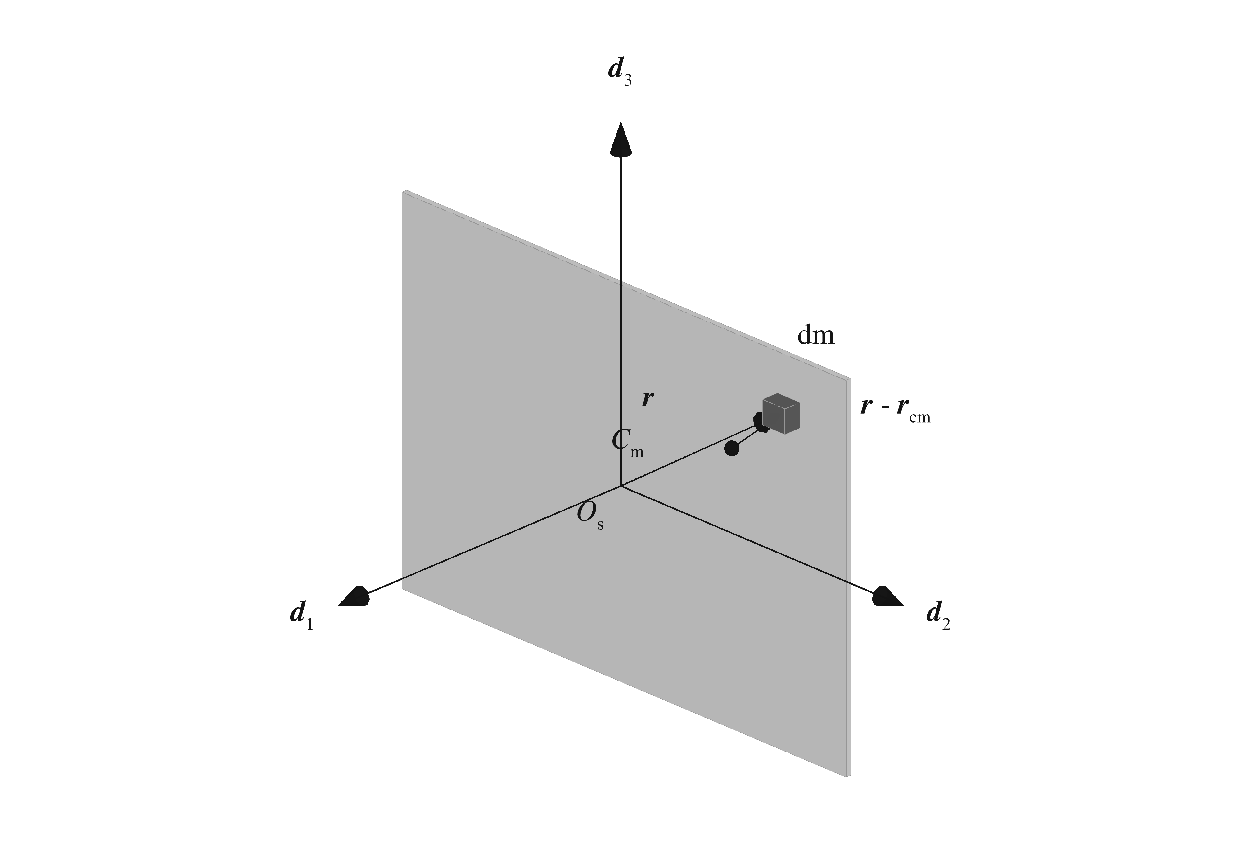
\includegraphics[width=.96\linewidth,height=.40\textheight,keepaspectratio]{figures/tecplot/concept_masa-seccional.pdf}
\caption[Geometría de la integración de masa]{Geometría de la integración de masa en una sección. $\vct r$ sitúa el elemento $\dd m$ respecto de $O_s$ y $\vct r-\vct r_{cm}$ lo sitúa respecto del centro de masa $C_m$. El espesor de la superficie y el tamaño del elemento de masa son ilustrativos.}\label{fig:masa-seccional}
\end{figure}

\section{Cuerpos rígidos tridimensionales}
Para una góndola o un cubo se integra sobre su volumen de referencia $V_0$:
\begin{align}
 m&=\int_{V_0}\rho_0\dd V_0,&
 \vct X_C&=\frac1m\int_{V_0}\rho_0\vct X\dd V_0,\\
 \ten J_C&=\int_{V_0}\rho_0\left[\|\vct X-\vct X_C\|^2\Id
 -(\vct X-\vct X_C)\otimes(\vct X-\vct X_C)\right]\dd V_0.
\end{align}
Ahora $m$ se expresa en $\mathrm{kg}$ y $\ten J_C$ en $\mathrm{kg\,m^2}$. La diferencia de mayúscula entre $\ten J_C$ y $\ten j_C$ distingue cantidades integradas en un volumen y cantidades por longitud, respectivamente.

Las propiedades obtenidas de un modelo geométrico tridimensional se expresan respecto de un origen, una base y un sistema de unidades determinados. El traslado al punto de referencia del cuerpo utiliza la identidad~\eqref{eq:steiner} con $\mu$ sustituido por $m$. El cambio de base del tensor completo se realiza mediante
\begin{equation}
 [\ten J_C]^A={}^A Q_B[\ten J_C]^B({}^A Q_B)^\tr.
\end{equation}
Primero se declara dónde está el centro y en qué base se conoce el tensor; luego se rota y traslada con esas mismas convenciones. Transformar solo tres valores diagonales ignora los productos de inercia generados por el cambio de orientación.

Para una representación mediante masas puntuales, la integral se aproxima por
\begin{equation}
 m\simeq\sum_k m_k,\quad
 \vct X_C\simeq m^{-1}\sum_k m_k\vct X_k,\quad
 \ten J_C\simeq\sum_k m_k\left[\|\vct r_k\|^2\Id-\vct r_k\otimes\vct r_k\right].
\end{equation}
Si cada componente tiene extensión finita, también debe sumarse su propio tensor centroidal rotado. Reemplazar cada componente por una masa puntual omite esa contribución. Una masa total por sí sola no permite reconstruir un tensor de inercia.

\section{Energía cinética y tensor de inercia de un cuerpo rígido}
\subsection{Posición de una partícula y centro de masa}
Considérese un cuerpo rígido con un punto de referencia $O$, solidario con el cuerpo, y centro de masa $C$. Para una partícula $P$ se definen los vectores $\vct r=\overrightarrow{OP}$, $\vct c=\overrightarrow{OC}$ y $\vct\rho=\overrightarrow{CP}$. Todos se consideran en la configuración actual y cumplen
\begin{equation}
 \vct r=\vct c+\vct\rho,\qquad
 \vct x_P=\vct x_O+\vct r=\vct x_C+\vct\rho.
 \label{eq:posicion-centromasa}
\end{equation}
Las componentes de $\vct r$ en una base solidaria permanecen constantes. En una base inercial varían con la orientación del cuerpo, por lo que el teorema de transporte proporciona
\begin{equation}
 \vct v_P=\vct v_O+\vct\omega\times\vct r
         =\vct v_C+\vct\omega\times\vct\rho,\qquad
 \vct v_C=\vct v_O+\vct\omega\times\vct c.
 \label{eq:velocidad-rigido-centro}
\end{equation}
La velocidad angular $\vct\omega$ es común a todas las partículas; sus velocidades lineales dependen de la distancia al eje instantáneo de rotación.

En la figura~\ref{fig:rigido-centro}, las posiciones absolutas y los vectores relativos se dibujan por separado para identificar las contribuciones a la velocidad de una partícula.

\begin{figure}[htbp]
\centering
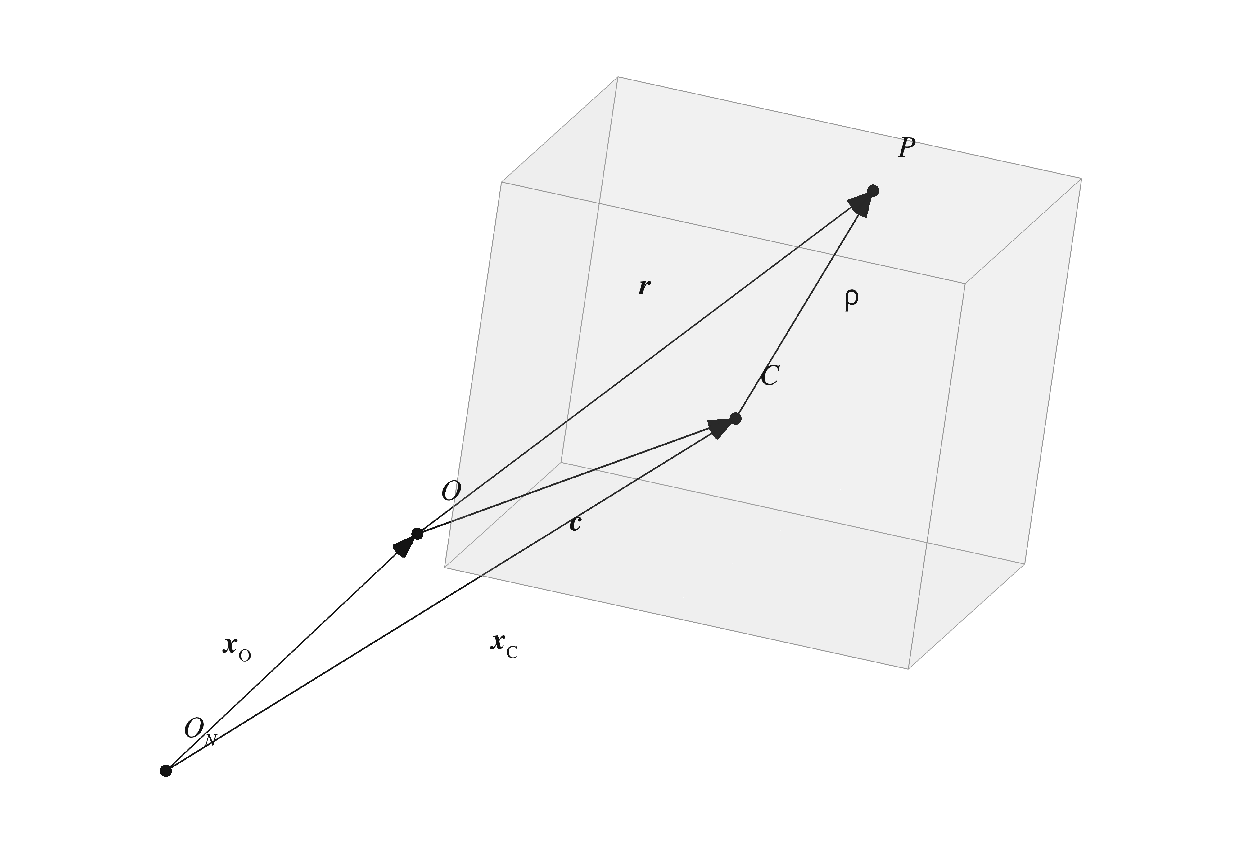
\includegraphics[width=.96\linewidth,height=.40\textheight,keepaspectratio]{figures/tecplot/concept_rigido-centro.pdf}
\caption[Posición de una partícula de cuerpo rígido]{Posiciones absolutas y relativas de una partícula de cuerpo rígido. Se cumple $\vct x_P=\vct x_O+\vct r=\vct x_C+\vct\rho$ y $\vct r=\vct c+\vct\rho$. La envolvente transparente sitúa el cuerpo y permite seguir los vectores desde el origen inercial $O_N$.}\label{fig:rigido-centro}
\end{figure}

Por definición del centro de masa,
\begin{equation}
 m\vct c=\int_{\mathcal B}\vct r\,\dd m,\qquad
 \int_{\mathcal B}\vct\rho\,\dd m
 =\int_{\mathcal B}(\vct r-\vct c)\,\dd m=\vct0.
 \label{eq:primer-momento-nulo}
\end{equation}
La medida $\dd m=\rho_0\dd V_0$ permanece constante durante el movimiento. Por ello la integración puede realizarse sobre la configuración de referencia, aunque los vectores se expresen en la configuración actual.

\subsection{Separación de traslación y rotación}
La energía cinética se obtiene integrando la contribución de cada partícula. Al sustituir la segunda forma de \eqref{eq:velocidad-rigido-centro},
\begin{align}
 T&=\frac12\int_{\mathcal B}\vct v_P\cdot\vct v_P\,\dd m\nonumber\\
 &=\frac12m\,\vct v_C\cdot\vct v_C
 +\vct v_C\cdot\left(\vct\omega\times
             \int_{\mathcal B}\vct\rho\,\dd m\right)
 +\frac12\int_{\mathcal B}\|\vct\omega\times\vct\rho\|^2\,\dd m.
 \label{eq:T-desarrollo}
\end{align}
El término cruzado es nulo por \eqref{eq:primer-momento-nulo}. Para el último término se emplea la identidad
\begin{equation}
 \|\vct\omega\times\vct\rho\|^2
 =\|\vct\omega\|^2\|\vct\rho\|^2-(\vct\omega\cdot\vct\rho)^2
 =\vct\omega\cdot
   \left[(\vct\rho\cdot\vct\rho)\Id-\vct\rho\otimes\vct\rho\right]\vct\omega.
\end{equation}
Así aparece el tensor de inercia respecto del centro de masa,
\begin{equation}
 \ten J_C=\int_{\mathcal B}
       \left[(\vct\rho\cdot\vct\rho)\Id-\vct\rho\otimes\vct\rho\right]\dd m,
 \qquad
 T=\frac12m\|\vct v_C\|^2+\frac12\vct\omega\cdot\ten J_C\vct\omega.
 \label{eq:T-centro}
\end{equation}
La primera contribución es la energía de traslación de una masa $m$ situada en $C$; la segunda recoge la distribución de esa masa alrededor de $C$. La separación es exacta para un cuerpo rígido.

En una base ortonormal con $\vct\rho=\rho_i\vct e_i$, las componentes son
\begin{equation}
 [\ten J_C]=\int_{\mathcal B}
 \begin{bmatrix}
 \rho_2^2+\rho_3^2&-\rho_1\rho_2&-\rho_1\rho_3\\
 -\rho_2\rho_1&\rho_1^2+\rho_3^2&-\rho_2\rho_3\\
 -\rho_3\rho_1&-\rho_3\rho_2&\rho_1^2+\rho_2^2
 \end{bmatrix}\dd m.
 \label{eq:J-componentes}
\end{equation}
Las entradas diagonales son momentos de inercia respecto de los ejes de la base. Las no diagonales son los negativos de los productos de inercia. Para un eje unitario $\vct n$, el momento respecto de ese eje es $\vct n\cdot\ten J_C\vct n$. Los ejes principales son los autovectores de $\ten J_C$; sus autovalores son los momentos principales de inercia y no deben confundirse con frecuencias naturales.

\subsection{Traslado a un punto de referencia arbitrario}
Al usar $\vct r=\vct c+\vct\rho$ en la definición de $\ten J_O$ aparecen términos cuadráticos en $\vct c$, términos cuadráticos en $\vct\rho$ y términos cruzados. Los últimos se anulan al integrar porque el primer momento de masa respecto de $C$ es cero. El resultado es el teorema de ejes paralelos:
\begin{equation}
 \ten J_O=\ten J_C+
 m\left[(\vct c\cdot\vct c)\Id-\vct c\otimes\vct c\right].
 \label{eq:Steiner-volumen}
\end{equation}
La energía expresada mediante la velocidad de $O$ contiene entonces una contribución de acoplamiento,
\begin{equation}
 T=\frac12m\|\vct v_O\|^2+
 m\,\vct v_O\cdot(\vct\omega\times\vct c)
 +\frac12\vct\omega\cdot\ten J_O\vct\omega.
 \label{eq:T-origen}
\end{equation}
Elegir el centro de masa como punto de referencia elimina este acoplamiento, pero no altera el movimiento físico. Elegir otro punto puede simplificar las conexiones mecánicas; en ese caso, la excentricidad debe conservarse tanto en la cinemática como en la matriz de masa.

\section{Matriz de masa y acoplamiento entre traslación y rotación}
En una sección rígida, la velocidad de un punto es
\begin{equation}
 \vct v(\vct\zeta)=\vct v_O+\vct\omega\times\vct\zeta.
\end{equation}
Se utilizan aquí vectores geométricos o componentes en una misma base. Al integrar $\frac12\rho_0\vct v\cdot\vct v$, se obtiene
\begin{equation}
 \mathcal T_s=\tfrac12\mu\vct v_O\cdot\vct v_O
 +\vct v_O\cdot(\vct\omega\times\vct h_m)
 +\tfrac12\vct\omega\cdot\ten j_O\vct\omega.
\end{equation}
Con el vector generalizado de velocidades $\vct\nu=[\vct v_O^\tr,\vct\omega^\tr]^\tr$,
\begin{equation}
 \mathcal T_s=\tfrac12\vct\nu^\tr\mathsf M_s\vct\nu,\qquad
 \mathsf M_s=
 \begin{bmatrix}
 \mu\Id&-\mu\sk{c_m}\\
 \mu\sk{c_m}&[\ten j_C]-\mu\sk{c_m}^{2}
 \end{bmatrix}.
 \label{eq:mass6}
\end{equation}
La matriz es simétrica porque $\sk{c_m}^\tr=-\sk{c_m}$. Sus bloques no comparten unidades: el bloque traslacional es $\mathrm{kg/m}$, el cruzado $\mathrm{kg}$ y el angular $\mathrm{kg\,m}$. Por esa razón se denomina matriz generalizada o espacial de masa y no tensor euclídeo ordinario de segundo orden de dimensión seis. La estructura en bloques conserva la interpretación tensorial de cada relación física.

\section{Rigidez seccional y resultantes}
Las fuerzas internas de una viga son resultantes de la distribución de tensiones en cada sección. Si $\vct t$ es la tracción sobre el corte y $\vct\zeta$ localiza un punto de ese corte respecto del origen seccional, las resultantes de fuerza y momento son
\begin{equation}
 \vct n=\int_A\vct t\,\dd A,\qquad
 \vct m=\int_A\vct\zeta\times\vct t\,\dd A.
 \label{eq:resultantes-seccion}
\end{equation}
En la descripción espacial, $\vct t=\ten\sigma\vct n_A$, donde $\ten\sigma$ es el tensor de tensiones de Cauchy y $\vct n_A$ es la normal unitaria al corte. La notación $\vct n_A$ se distingue de la resultante $\vct n$. Para pequeñas deformaciones, las resultantes se expresan en la base de sección y se relacionan con sus medidas de extensión, cortante, torsión y flexión mediante una ley constitutiva unidimensional.

En un material elástico lineal, la relación tridimensional tiene la forma $\sigma_{ij}=\mathbb C_{ijkl}\varepsilon_{kl}$, con $\mathbb C$ el tensor de elasticidad de cuarto orden. La integración en la sección transforma esa relación en una ley entre seis resultantes y seis deformaciones generalizadas. Para una sección heterogénea o laminada, la distribución de material y la deformación local intervienen en esa reducción; sus propiedades no quedan determinadas únicamente por el contorno exterior.
Las medidas $\vct\gamma$ y $\vct\kappa$, definidas en el capítulo de cinemática, tienen unidades adimensionales y $\mathrm{m^{-1}}$. Sus resultantes conjugadas son fuerza $\vct n$ y momento $\vct m$; la potencia interna por longitud tiene la forma
\begin{equation}
 \mathcal P_{\rm int,s}=\vct n\cdot\dot{\vct\gamma}+\vct m\cdot\dot{\vct\kappa}.
\end{equation}
En elasticidad seccional lineal se escribe una relación en bloques tensoriales:
\begin{equation}
 \begin{bmatrix}\vct n\\\vct m\end{bmatrix}=
 \underbrace{\begin{bmatrix}
 \ten C_{\gamma\gamma}&\ten C_{\gamma\kappa}\\
 \ten C_{\kappa\gamma}&\ten C_{\kappa\kappa}
 \end{bmatrix}}_{\mathsf C_s}
 \begin{bmatrix}\vct\gamma\\\vct\kappa\end{bmatrix}.
 \label{eq:Csection}
\end{equation}
Los bloques tienen unidades $\mathrm N$, $\mathrm{N\,m}$, $\mathrm{N\,m}$ y $\mathrm{N\,m^2}$. En un material elástico recíproco, $\ten C_{\kappa\gamma}=\ten C_{\gamma\kappa}^\tr$ y los bloques diagonales son simétricos. La rigidez de una pala laminada puede contener acoplamiento extensión--torsión o flexión--torsión. Una matriz diagonal no los representa.

Para una sección homogénea, isotrópica, con ejes centroidales principales, línea de referencia adecuada y acoplamientos despreciables, se adopta
\begin{equation}
 \mathsf C_s=\diag(EA,\,G A_{s2},\,G A_{s3},\,GJ_t,\,EI_2,\,EI_3).
\end{equation}
Aquí $E$ es el módulo de Young y $G=E/[2(1+\nu)]$ para material isotrópico. Las áreas $A_{s2}=k_2A$ y $A_{s3}=k_3A$ incorporan factores efectivos de cortante. Si una tabla ya suministra $GA_{s2}$, no se multiplica de nuevo por $k_2$. En palas compuestas, las rigideces pueden proceder de una homogeneización seccional; no es necesario ni siempre posible reconstruir un único $E$ equivalente.

Para una torre tubular circular de radios $R_o$ y $R_i$,
\begin{equation}
 A=\pi(R_o^2-R_i^2),\quad I_2=I_3=\frac\pi4(R_o^4-R_i^4),\quad
 J_t=\frac\pi2(R_o^4-R_i^4).
\end{equation}
Estas fórmulas ilustran un caso en que área, flexión y torsión se deducen de la geometría. No se trasladan a una pala simplemente por conocer su cuerda.

\section{Distribución de propiedades a lo largo de las palas}
Cada estación seccional debe identificar $S$, origen, orientación, unidades, $\mu$, $\vct c_m$, $\ten j_C$ y $\mathsf C_s$. Si faltan excentricidades o productos de inercia, asignarlos a cero constituye una hipótesis, no una medición. Si se ajusta una distribución de densidad a una masa objetivo mediante un factor $c$, todas las propiedades lineales en densidad deben escalar de manera compatible: $\mu\mapsto c\mu$, $\vct h_m\mapsto c\vct h_m$, $\ten j_C\mapsto c\ten j_C$. El centro de masa permanece igual. Ese ajuste no modifica automáticamente las rigideces.

La masa de una pala es $m_b=\int_0^{L_b}\mu(S)\dd S$. Su inercia global exige además trasladar cada sección al punto de interés e integrar; no equivale a $\int\ten j_C\dd S$ sin las contribuciones orbitales. Esta distinción es decisiva en un rotor, donde gran parte de la inercia respecto al eje procede de la distancia radial de las secciones.

\chapter{Formulación mediante elementos finitos}
\label{ch:elementos}

La descripción continua identifica puntos materiales, líneas de referencia y
orientaciones de sección sin introducir nodos. La discretización constituye un
paso posterior: sustituye los campos desconocidos por aproximaciones definidas
mediante un número finito de parámetros. Por ello, un nodo no es una partícula
adicional del cuerpo ni una unión física necesariamente existente. Es una
estación de interpolación de la línea de referencia. Una unión entre cuerpos,
en cambio, requiere una condición cinemática o una ley mecánica específica.

Este capítulo desarrolla la especialización a elementos rectos de viga de
Timoshenko con dos nodos. Se separan la interpolación de los campos, las
propiedades que relacionan deformaciones y resultantes, y las restricciones
entre componentes. Los fundamentos de aproximación y ensamblaje corresponden
al método de elementos finitos \cite{reddy}; la descripción de vínculos rígidos
se inscribe en la cinemática de sistemas multicuerpo \cite{shabana}. Las fórmulas
cerradas corresponden a elementos rectos de propiedades constantes, con
extensión, torsión y flexión con deformación por cortante.

\section{Del cuerpo continuo a la malla de vigas}

Sea $S$ la coordenada material longitudinal de la torre o de una pala en la
configuración de referencia. Se divide su intervalo en subintervalos
$[S_I,S_J]$, de longitud $L=S_J-S_I>0$ para el elemento recto considerado.
Dentro de cada elemento se emplea $s=S-S_I\in[0,L]$. La discretización puede
aproximar mediante segmentos una línea inicialmente curva, pero las expresiones
cerradas siguientes corresponden a cada segmento recto, no a un elemento curvo
exacto. Los cambios de geometría o propiedades deben ser representados mediante
la partición o mediante una formulación que los admita explícitamente.

La figura~\ref{fig:continuo-malla} distingue la línea material continua de su partición en elementos; los nodos parametrizan la aproximación del movimiento.

\begin{figure}[htbp]
\centering
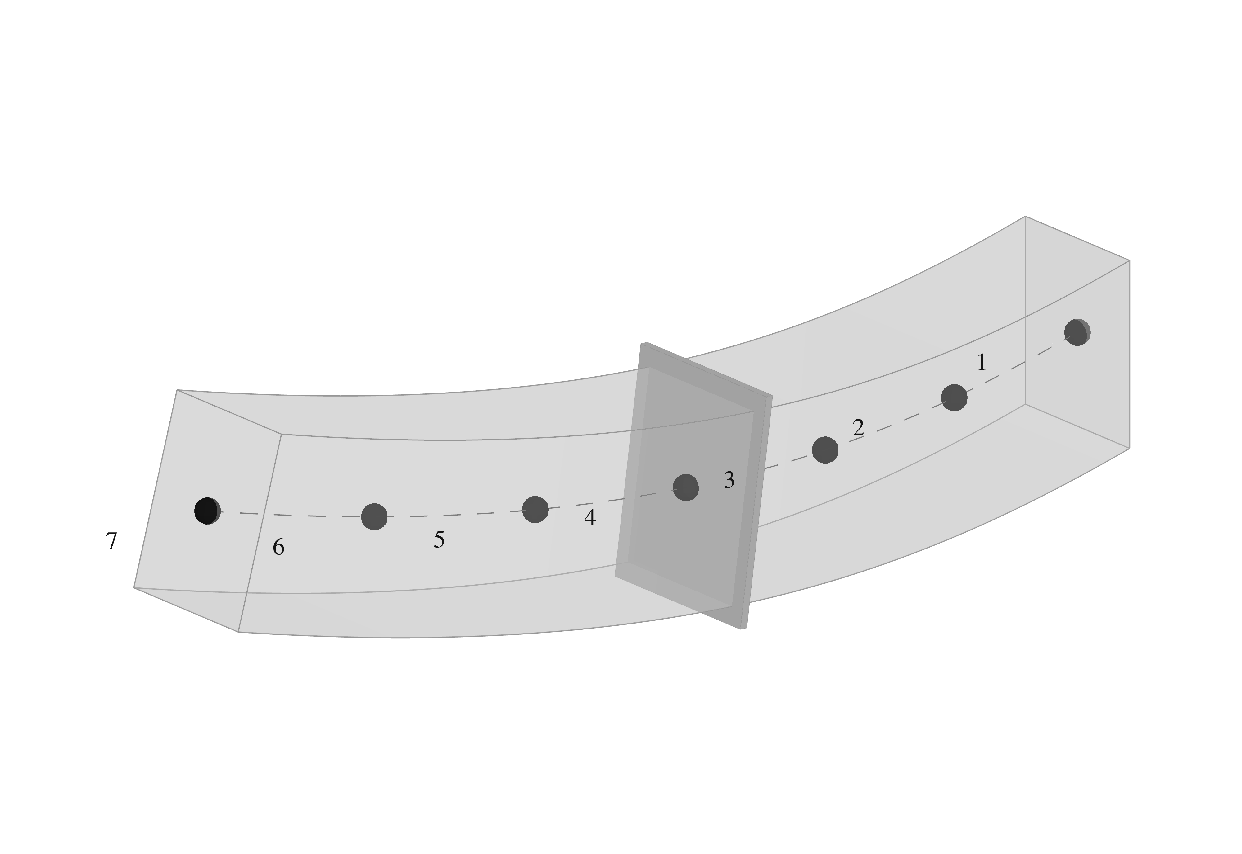
\includegraphics[width=.96\linewidth,height=.40\textheight,keepaspectratio]{figures/tecplot/concept_continuo-malla.pdf}
\caption[Descripción continua y discretización]{Envolvente de una viga, línea material de referencia y nodos de una partición espacial. Los números siguen el orden material de los nodos. El movimiento de la sección señalada se recupera mediante las coordenadas nodales. La superficie es ilustrativa y no representa elementos sólidos.}\label{fig:continuo-malla}
\end{figure}

En componentes locales se agrupan las perturbaciones de un nodo como
\begin{equation}
 \vct q_i^e=[u_{1i},u_{2i},u_{3i},\theta_{1i},\theta_{2i},\theta_{3i}]^{\tr},
 \qquad
 \vct q_e=[(\vct q_I^e)^{\tr},(\vct q_J^e)^{\tr}]^{\tr}.
\end{equation}
El superíndice $e$ indica componentes en la base local del elemento. Existen
doce coordenadas elementales antes de ensamblar e imponer vínculos: tres
traslaciones y tres pequeñas rotaciones por nodo. No son doce movimientos
independientes después de imponer un empotramiento o de identificar una raíz
con un cubo rígido. Tampoco incluyen el azimut nominal prescrito del rotor
como una incógnita adicional.

La hipótesis de Timoshenko permite que la normal a la sección y la tangente a
la línea deformada difieran. Se retienen extensión, dos deformaciones por
cortante, torsión y dos curvaturas. No se incorporan como incógnitas
independientes el alabeo de la sección, su distorsión en el plano o modos
locales de una pared. La reducción a viga debe interpretarse con estas
delimitaciones, aunque las propiedades seccionales procedan de un cálculo
tridimensional más detallado.

La figura~\ref{fig:coordenadas-nodo} separa las coordenadas de traslación de las coordenadas angulares de un nodo. Cada una multiplica una dirección local definida; la orientación del elemento permite después expresar todas en la base de ensamblaje. Una coordenada angular nodal describe el giro de la sección, no una pendiente impuesta de la línea.

\begin{figure}[htbp]
\centering
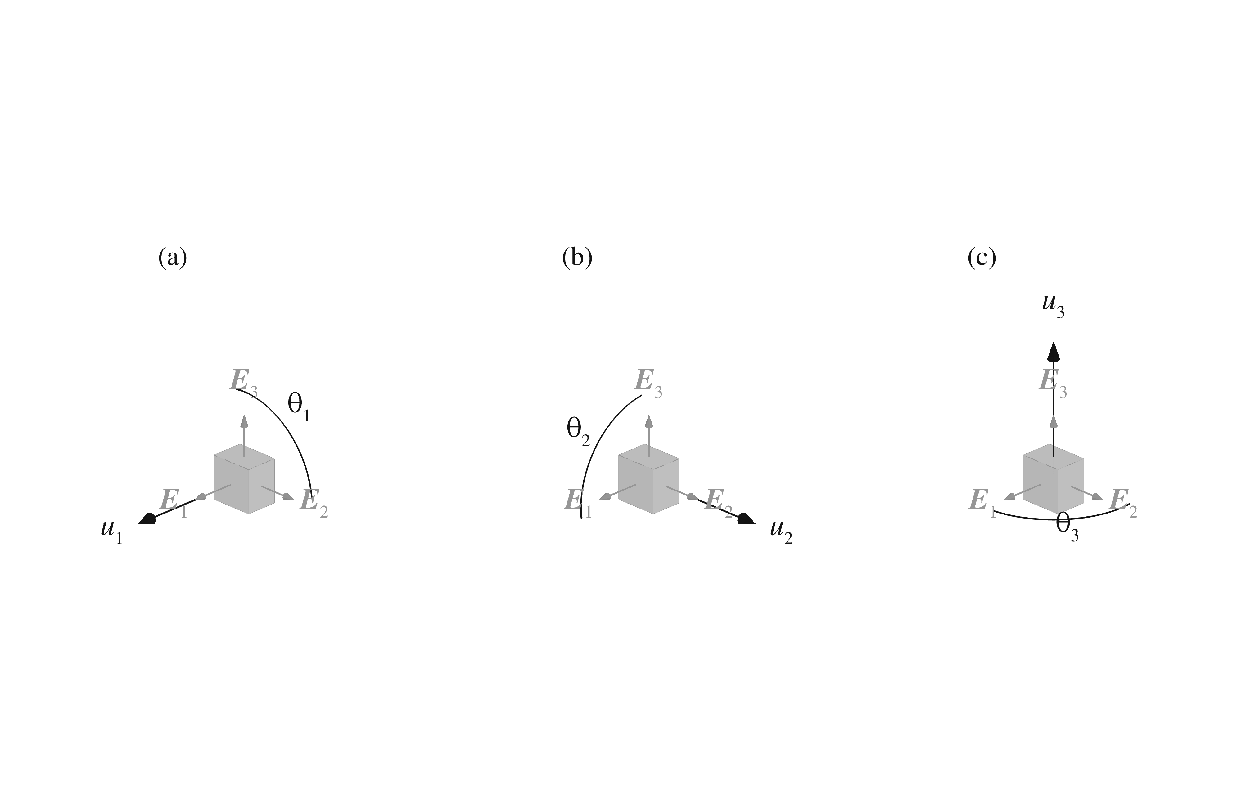
\includegraphics[width=.96\linewidth,height=.40\textheight,keepaspectratio]{figures/tecplot/concept_coordenadas-nodo.pdf}
\caption[Coordenadas de traslación y rotación de un nodo]{Las seis coordenadas de un nodo se organizan por dirección: (a) $u_1,\theta_1$, (b) $u_2,\theta_2$ y (c) $u_3,\theta_3$. La flecha recta representa una traslación y el arco una rotación alrededor del eje correspondiente. Las amplitudes se amplían y no constituyen una respuesta simultánea calculada.}\label{fig:coordenadas-nodo}
\end{figure}

\section{Interpolación y medidas de deformación}

El campo seccional aproximado se escribe
\begin{equation}
 \vct\eta(s)=
 [u_1,u_2,u_3,\theta_1,\theta_2,\theta_3]^{\tr}
 =\ten N(s)\vct q_e.
 \label{eq:fe-campo}
\end{equation}
Las traslaciones tienen dimensión de longitud y las rotaciones son
adimensionales. En consecuencia, algunas entradas de $\ten N$ que convierten
una rotación nodal en desplazamiento llevan dimensiones de longitud. No debe
interpretarse toda la matriz como una colección de funciones adimensionales.

En la aproximación lineal alrededor de una referencia recta, con ejes
dextrógiros y eje 1 longitudinal,
\begin{equation}
 \vct\varepsilon=
 \begin{bmatrix}u_{1,s}\\u_{2,s}-\theta_3\\u_{3,s}+\theta_2\\
 \theta_{1,s}\\\theta_{2,s}\\\theta_{3,s}\end{bmatrix}
 =\mathcal D\vct\eta=\ten B(s)\vct q_e,
 \qquad \ten B=\mathcal D\ten N.
 \label{eq:fe-strain}
\end{equation}
Aquí $\mathcal D$ es un operador diferencial explícito: deriva los campos
respecto de $s$ y combina las rotaciones con las pendientes transversales.
Las tres primeras entradas son deformaciones adimensionales y las tres
últimas tienen dimensión de inverso de longitud. La coexistencia de ambos
tipos explica las diferentes unidades de los bloques de rigidez seccional.

La interpolación más simple utiliza
$N_I=1-s/L$, $N_J=s/L$ y
$\ten N_{\rm lin}=[N_I\Id_6,N_J\Id_6]$. Por ejemplo,
\begin{equation}
 \gamma_2=\frac{u_{2J}-u_{2I}}{L}-N_I\theta_{3I}-N_J\theta_{3J}.
\end{equation}
La derivada del desplazamiento es constante, mientras que la rotación es
lineal. Cuando la viga se hace esbelta, imponer cortante prácticamente nulo en
todo el elemento restringe excesivamente esa combinación y puede producir
\emph{bloqueo por cortante}: la aproximación resulta artificialmente rígida.
No se trata de una propiedad física del material. Una opción es integrar
selectivamente la energía de cortante; otra es utilizar interpolaciones
compatibles con la solución del elemento. Ambas opciones son formulaciones
distintas y no deben combinarse sin justificar la operación.

La figura~\ref{fig:interpolacion-lineal} ilustra el significado de las funciones $N_I$ y $N_J$. En cada extremo se recupera exactamente el valor nodal correspondiente. En el interior, el valor se calcula mediante una combinación ponderada; no se introduce una nueva incógnita en cada sección. Esta ilustración corresponde a la interpolación lineal recién definida, no a las funciones cerradas de flexión que se deducen a continuación.

\begin{figure}[htbp]
\centering
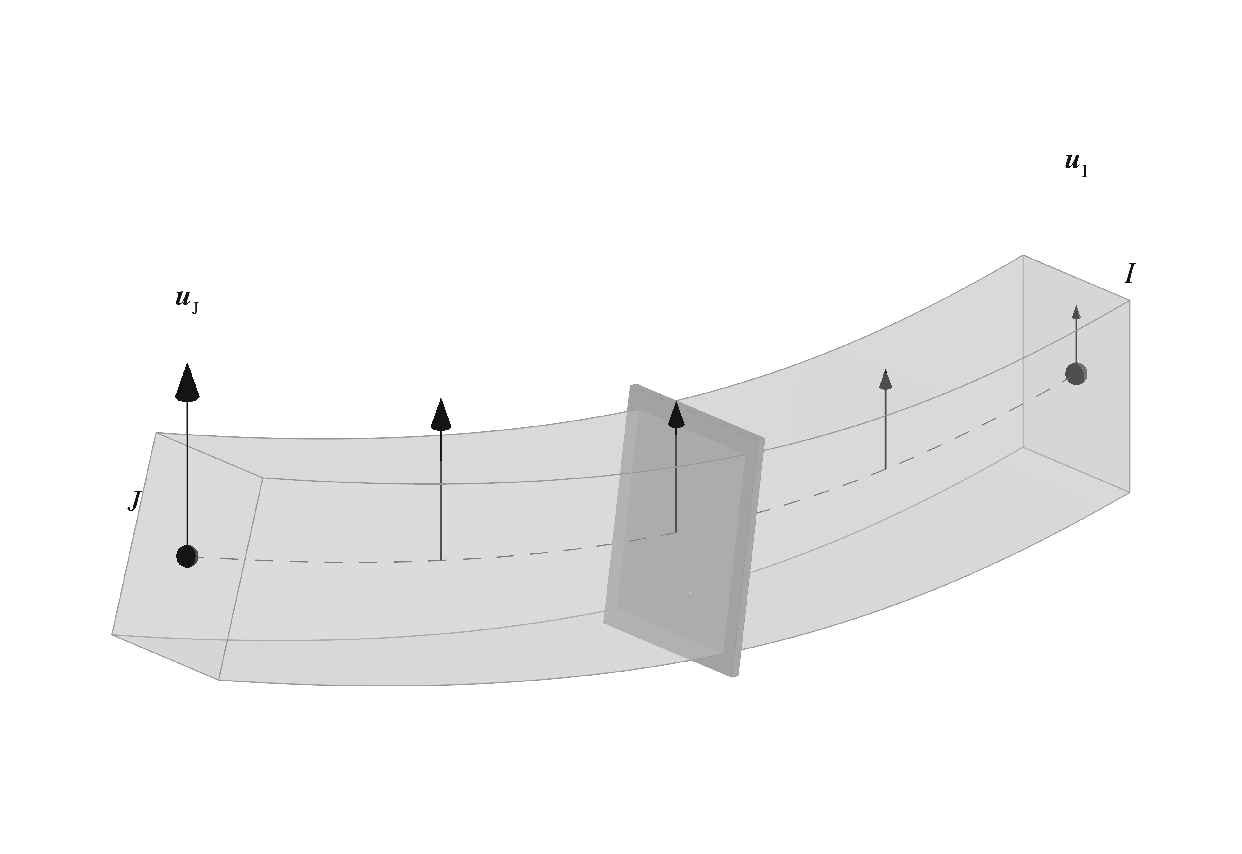
\includegraphics[width=.96\linewidth,height=.40\textheight,keepaspectratio]{figures/tecplot/concept_interpolacion-lineal.pdf}
\caption[Interpolación entre valores nodales]{Interpolación de un campo de desplazamientos entre los valores nodales $\vct u_I$ y $\vct u_J$. Las flechas intermedias ilustran $\vct u(S)=N_I(S)\vct u_I+N_J(S)\vct u_J$. La línea curva y la envolvente son esquemáticas; las expresiones elementales cerradas del texto corresponden a segmentos rectos.}\label{fig:interpolacion-lineal}
\end{figure}

\section{Especialización de propiedades constantes: interpolación cerrada}

La interpolación se obtiene de la solución estática homogénea de la viga de
Timoshenko, con propiedades constantes y desacopladas en cada elemento.
En el plano $(1,2)$ intervienen $EI_3$ y
$GA_{s2}$; se definen
\begin{equation}
 \phi_2=\frac{12EI_3}{GA_{s2}L^2},\quad
 \zeta=\frac{s}{L},\quad
 \vct p=[1,\zeta,\zeta^2,\zeta^3],\quad
 \vct d_2=[u_{2I},\theta_{3I},u_{2J},\theta_{3J}]^{\tr}.
\end{equation}
Para obtener las funciones de interpolación se considera primero un tramo sin carga distribuida. En el plano $(1,2)$, sus ecuaciones de equilibrio y constitutivas son
\begin{equation}
 n_2'=0,\qquad m_3'+n_2=0,\qquad
 n_2=GA_{s2}(u_2'-\theta_3),\qquad m_3=EI_3\theta_3'.
\end{equation}
Con propiedades constantes, la fuerza cortante $n_2$ es constante, el momento $m_3$ es lineal, la rotación $\theta_3$ es cuadrática y el desplazamiento $u_2$ es cúbico. Las cuatro constantes independientes se determinan imponiendo los valores de $u_2$ y $\theta_3$ en ambos extremos. La expresión matricial que sigue reúne esa solución en términos de las cuatro coordenadas nodales.

El parámetro $\phi_2$ cuantifica la contribución del cortante en relación con
la flexión para la longitud del elemento. Las áreas $A_{s2}$ y $A_{s3}$ son
áreas efectivas: si incluyen factores de corrección, estos no vuelven a
multiplicarse. Para un valor genérico $\phi$, sean
\begin{equation}
 \ten C_v=\frac{1}{1+\phi}
 \begin{bmatrix}
 1+\phi&0&0&0\\
 -\phi&L(1+\phi/2)&\phi&-L\phi/2\\
 -3&-L(2+\phi/2)&3&-L(1-\phi/2)\\
 2&L&-2&L
 \end{bmatrix},
\end{equation}
\begin{equation}
 \ten C_r=\frac{1}{1+\phi}
 \begin{bmatrix}
 0&1+\phi&0&0\\
 -6/L&-(4+\phi)&6/L&-(2-\phi)\\
 6/L&3&-6/L&3\\
 0&0&0&0
 \end{bmatrix}.
\end{equation}
Entonces $u_2=\vct p\ten C_v\vct d_2$ y
$\theta_3=\vct p\ten C_r\vct d_2$, usando $\phi=\phi_2$.
Estas funciones reproducen las coordenadas en ambos extremos y permiten
pendiente y rotación diferentes. La palabra ``exacta'' se refiere a la
solución estática homogénea del elemento recto de propiedades constantes que
genera estas funciones; no afirma que una malla finita reproduzca exactamente
todos los campos dinámicos o todas las cargas distribuidas.

En el plano $(1,3)$ se utiliza
\begin{equation}
 \phi_3=\frac{12EI_2}{GA_{s3}L^2},\quad
 \vct d_3=[u_{3I},\theta_{2I},u_{3J},\theta_{2J}]^{\tr},\quad
 \ten S_- =\diag(1,-1,1,-1),
\end{equation}
\begin{equation}
 u_3=\vct p\ten C_v\ten S_-\vct d_3,\qquad
 \theta_2=-\vct p\ten C_r\ten S_-\vct d_3,
 \qquad \phi=\phi_3.
\end{equation}
Los signos provienen de $\gamma_3=u_{3,s}+\theta_2$ y de la orientación de la
base, no de una diferencia física entre ambos planos. Finalmente, $u_1$ y
$\theta_1$ se interpolan con $N_I,N_J$. Estas seis relaciones definen todas
las entradas de $\ten N$; aplicar \eqref{eq:fe-strain} determina $\ten B$.

\section{Rigidez, masa y cargas elementales}

\subsection{Balance elemental y trabajo virtual}

Antes de construir matrices, se establece qué ecuaciones se aproximan. Sean
$\vct n(s)$ la fuerza interna de sección, $\vct m(s)$ el momento interno,
$\vct p(s)$ la fuerza externa por longitud y $\vct\ell(s)$ el momento externo
por longitud. Todos se expresan en la misma base local. Se adopta
\begin{equation}
 \vct t_s=\begin{bmatrix}\vct n\\\vct m\end{bmatrix}
 =\mathsf C_s\vct\varepsilon,
 \qquad
 \vct f_s=\begin{bmatrix}\vct p\\\vct\ell\end{bmatrix},
\end{equation}
donde $\mathsf C_s$ es la matriz seccional definida en el capítulo anterior.
El vector $\vct\ell$ no es una resultante interna: representa, por ejemplo,
un momento aerodinámico distribuido. Esta distinción evita confundir unidades
y acciones que intervienen en lados diferentes del balance.

Una variación virtual $\delta\vct\eta=[\delta\vct u^{\tr},
\delta\vct\theta^{\tr}]^{\tr}$ es un campo arbitrario compatible con los
vínculos homogéneos; no es una derivada temporal ni el movimiento real durante
un intervalo de tiempo. En esta subsección el símbolo $\delta$ denota la
variación de prueba. Las variaciones de deformación son
\begin{equation}
 \delta\vct\gamma=\delta\vct u_{,s}
 +\vct e_1\times\delta\vct\theta,
 \qquad
 \delta\vct\kappa=\delta\vct\theta_{,s}.
\end{equation}
Por tanto, el trabajo virtual interno toma la forma
\begin{align}
 \delta W_{\rm int}
 &=\int_0^L(\delta\vct\gamma\cdot\vct n
       +\delta\vct\kappa\cdot\vct m)\,\dd s\nonumber\\
 &=[\delta\vct u\cdot\vct n+
       \delta\vct\theta\cdot\vct m]_0^L\nonumber\\
 &\quad-\int_0^L\left[\delta\vct u\cdot\vct n_{,s}
       +\delta\vct\theta\cdot
       (\vct m_{,s}+\vct e_1\times\vct n)\right]\dd s.
 \label{eq:fe-partes}
\end{align}
La integración por partes revela el término de equilibrio de momentos
$\vct e_1\times\vct n$. Este término es precisamente la contraparte estática
del cortante de Timoshenko. No aparece al tratar traslaciones y rotaciones
como campos completamente independientes de la medida de deformación.

Sean $\vct i_u$ y $\vct i_\theta$ las resultantes inerciales por longitud.
El principio de trabajo virtual dinámico establece
\begin{equation}
 \int_0^L\delta\vct\varepsilon^{\tr}\vct t_s\,\dd s
 +\int_0^L\delta\vct\eta^{\tr}
        \begin{bmatrix}\vct i_u\\\vct i_\theta\end{bmatrix}\dd s
 =\int_0^L\delta\vct\eta^{\tr}\vct f_s\,\dd s
 +\delta W_{\partial e}.
 \label{eq:fe-debil}
\end{equation}
Para variaciones nulas en los extremos, \eqref{eq:fe-partes} conduce a los
balances locales
\begin{equation}
 \vct n_{,s}+\vct p=\vct i_u,\qquad
 \vct m_{,s}+\vct e_1\times\vct n+\vct\ell=\vct i_\theta.
\end{equation}
En los extremos libres de condiciones esenciales, el término de borde
identifica fuerzas y momentos aplicados: $(-\vct n,-\vct m)$ en $s=0$ y
$(\vct n,\vct m)$ en $s=L$. En un desplazamiento o giro impuesto, la variación
correspondiente se anula y la reacción se recupera posteriormente del
residual. Así se distinguen condiciones esenciales y naturales sin imponer
ambas a una misma coordenada de extremo.

Para pequeñas perturbaciones alrededor de una referencia estacionaria, sin
giro nominal y con base fija, las inercias son
$[\vct i_u^{\tr},\vct i_\theta^{\tr}]^{\tr}
=\mathsf M_s\ddot{\vct\eta}$, donde $\mathsf M_s$ es la matriz espacial del
capítulo anterior. El caso rotatorio incorpora términos adicionales de
transporte y velocidad; no se obtiene omitiéndolos en esta expresión
estacionaria. Sustituyendo $\vct\eta=\ten N\vct q_e$ y
$\delta\vct\eta=\ten N\delta\vct q_e$ en \eqref{eq:fe-debil}, para
$\ten N$ independiente del tiempo, se obtiene
\begin{equation}
 \delta\vct q_e^{\tr}
 (\ten M_e\ddot{\vct q}_e+\ten K_e\vct q_e
       -\vct f_e-\vct f_{\partial e})=0.
\end{equation}
La arbitrariedad de las coordenadas virtuales admisibles produce las
ecuaciones nodales. La forma débil es, por consiguiente, el vínculo entre los
balances continuos y las matrices que siguen; la energía elástica es una
representación equivalente de la contribución interna cuando
$\mathsf C_s$ es simétrica.

\subsection{Matrices elementales y cargas consistentes}

Si $\mathsf C_s$ es la matriz constitutiva seccional en la base local, la energía
elástica y su matriz elemental son
\begin{equation}
 U_e=\frac12\int_0^L\vct\varepsilon^{\tr}\mathsf C_s\vct\varepsilon\,\dd s
 =\frac12\vct q_e^{\tr}\ten K_e\vct q_e,
 \qquad
 \ten K_e=\int_0^L\ten B^{\tr}\mathsf C_s\ten B\,\dd s.
\end{equation}
Para $\mathsf C_s=\diag(EA,GA_{s2},GA_{s3},GJ_t,EI_2,EI_3)$, la extensión y la
torsión aportan, respectivamente,
\begin{equation}
 \ten K_{\rm ax}=\frac{EA}{L}\begin{bmatrix}1&-1\\-1&1\end{bmatrix},
 \qquad
 \ten K_{\rm tor}=\frac{GJ_t}{L}\begin{bmatrix}1&-1\\-1&1\end{bmatrix}.
\end{equation}
Se insertan en los índices $(1,7)$ y $(4,10)$ de $\vct q_e$. Para cada plano,
con sus valores de $EI$, $GA_s$ y $\phi=12EI/(GA_sL^2)$, se definen
\begin{equation}
 a=\frac{12EI}{L^3(1+\phi)},\quad b=\frac{6EI}{L^2(1+\phi)},\quad
 c=\frac{(4+\phi)EI}{L(1+\phi)},\quad d=\frac{(2-\phi)EI}{L(1+\phi)}.
\end{equation}
La contribución de flexión y cortante es
\begin{equation}
 \ten K_{\rm fl}=\begin{bmatrix}
 a&\sigma b&-a&\sigma b\\
 \sigma b&c&-\sigma b&d\\
 -a&-\sigma b&a&-\sigma b\\
 \sigma b&d&-\sigma b&c
 \end{bmatrix}.
\end{equation}
Se emplea $\sigma=1$, $EI=EI_3$ en los índices $(2,6,8,12)$ y
$\sigma=-1$, $EI=EI_2$ en $(3,5,9,11)$. Los cuatro bloques construyen la
matriz completa. Para una sección acoplada se conserva la integral general y
se elige una interpolación adecuada; no basta con agregar arbitrariamente
entradas a estos bloques desacoplados.

La masa seccional $\mathsf M_s$, construida con masa por longitud, tensor
centroidal y excentricidad, produce la matriz consistente
\begin{equation}
 \ten M_e=\int_0^L\ten N^{\tr}\mathsf M_s\ten N\,\dd s.
 \label{eq:fe-masa}
\end{equation}
``Consistente'' significa que se utiliza el mismo campo cinemático que
describe el movimiento. No implica concentrar toda la masa en los nodos. La
inercia rotacional permanece aunque el cortante tienda a cero; ese límite
dinámico corresponde a una viga con inercia rotacional, y no automáticamente
al modelo clásico de Euler--Bernoulli sin ella. Con propiedades constantes,
los productos polinómicos de la masa tienen grado máximo seis y cuatro puntos
de Gauss los integran exactamente. Si las propiedades varían, esta afirmación
de exactitud ya no se deduce únicamente del grado de $\ten N$.

Una distribución de fuerza $\vct p$ y momento $\vct\ell$ por longitud genera
\begin{equation}
 \vct f_e=\int_0^L\ten N^{\tr}
 \begin{bmatrix}\vct p\\\vct\ell\end{bmatrix}\dd s.
\end{equation}
Esta equivalencia se establece por igualdad de trabajo virtual, no por un
reparto intuitivo entre extremos. Si la carga depende de la configuración o
velocidad, también deben evaluarse sus derivadas al linealizar las ecuaciones.

\section{Cambio de componentes y ensamblaje}

La figura~\ref{fig:elemento} relaciona el intervalo material con la base espacial de un elemento recto. Para fijar esa base se utilizan los extremos $\vct X_I,\vct X_J$ y un punto auxiliar $\vct X_a$ fuera de su recta:
\begin{align}
 L&=\|\vct X_J-\vct X_I\|,\qquad
 \vct e_1=(\vct X_J-\vct X_I)/L,\nonumber\\
 \vct p&=(\Id-\vct e_1\otimes\vct e_1)(\vct X_a-\vct X_I),\nonumber\\
 \vct e_3&=\vct p/\|\vct p\|,\qquad
 \vct e_2=\vct e_3\times\vct e_1.
 \label{eq:base-geometrica-elemento}
\end{align}
El punto auxiliar fija las direcciones transversales y debe elegirse de acuerdo con la orientación de las propiedades seccionales. No es un nodo estructural ni agrega coordenadas al elemento. La construcción exige $\|\vct p\|>0$; un punto alineado con los extremos no permite definir una base.
\begin{figure}[htbp]
\centering
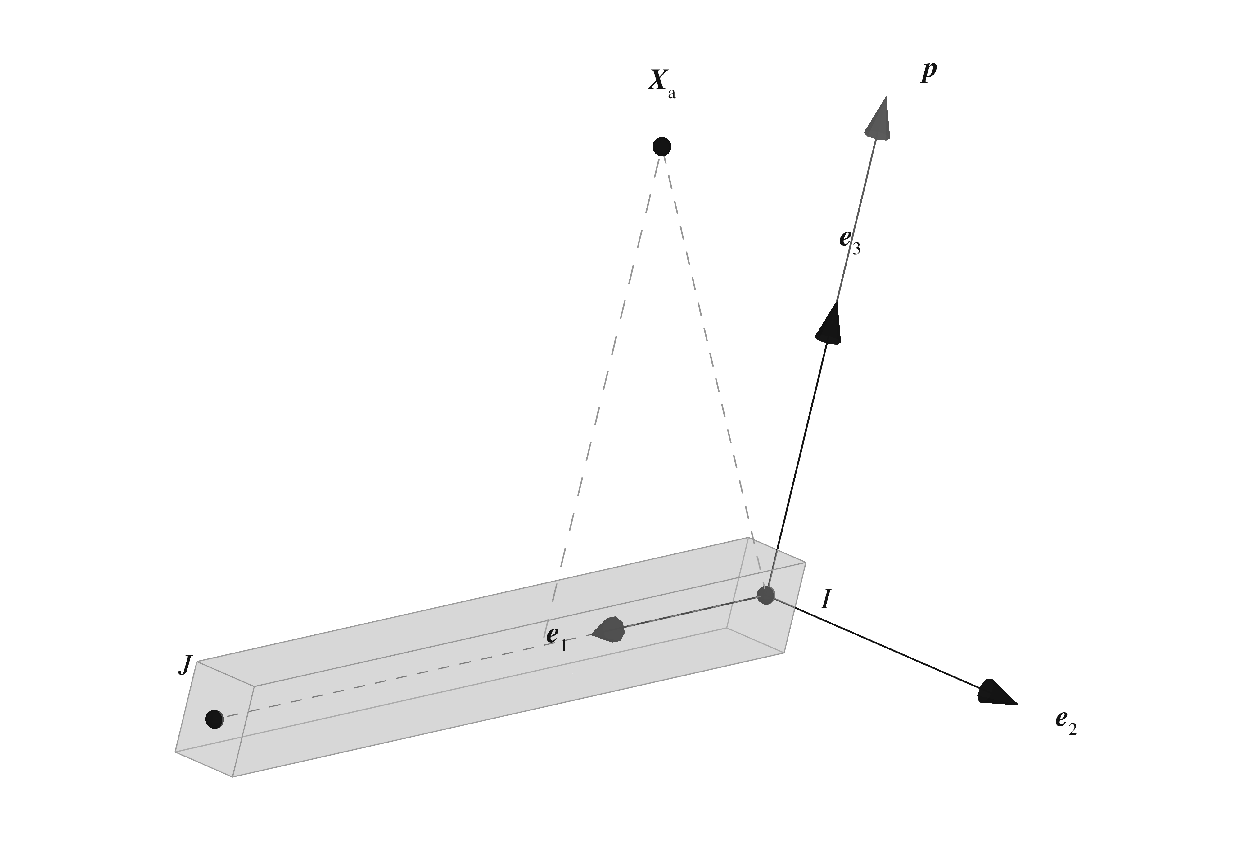
\includegraphics[width=.96\linewidth,height=.40\textheight,keepaspectratio]{figures/tecplot/concept_elemento.pdf}
\caption[Discretización y sistema local del elemento]{Orientación espacial de un elemento entre los nodos $I$ y $J$. El punto auxiliar $\vct X_a$ define una dirección transversal mediante su proyección $\vct p$ sobre el plano normal a $\vct e_1$. $\vct e_3$ es paralelo a $\vct p$ y $\vct e_2=\vct e_3\times\vct e_1$. El punto auxiliar no añade grados de libertad.}\label{fig:elemento}
\end{figure}

Sean las columnas de $\ten Q_e$ los ejes locales expresados en el sistema de referencia
newtoniano $\mathcal F_N$. Entonces $\vct v^N=\ten Q_e\vct v^e$ y
\begin{equation}
 \vct q_e=\ten T_e\vct q_e^N,\qquad
 \ten T_e=\diag(\ten Q_e^{\tr},\ten Q_e^{\tr},
                    \ten Q_e^{\tr},\ten Q_e^{\tr}).
\end{equation}
En una configuración fijada, $\ten K_e^N=\ten T_e^{\tr}\ten K_e\ten T_e$,
$\ten M_e^N=\ten T_e^{\tr}\ten M_e\ten T_e$ y
$\vct f_e^N=\ten T_e^{\tr}\vct f_e$. Son cambios de componentes, no
aproximaciones adicionales. Si la base gira, las ecuaciones dinámicas requieren
además las derivadas temporales de la transformación, como se explicita más adelante.

La matriz de conectividad $\ten L_e$ extrae del vector global $\vct q$ las
coordenadas del elemento: $\vct q_e^N=\ten L_e\vct q$. El ensamblaje suma
contribuciones que realizan trabajo sobre las mismas coordenadas:
\begin{equation}
 \ten K=\sum_e\ten L_e^{\tr}\ten K_e^N\ten L_e+\ten K_{\rm uniones},
 \qquad
 \ten M=\sum_e\ten L_e^{\tr}\ten M_e^N\ten L_e+\ten M_{\rm cuerpos}.
\end{equation}
Las masas de góndola y cubo y las leyes del tren o la base se incorporan
mediante sus relaciones de conexión. La coincidencia espacial de dos puntos no
impone por sí sola igualdad de desplazamientos: debe existir una conectividad
compartida o una restricción declarada.

\section{Vínculos entre el cubo y las raíces de las palas}

Se utiliza el punto de referencia del cubo como maestro cinemático; las raíces
son puntos dependientes. ``Maestro'' y ``esclavo'' describen la elección de
coordenadas independientes y no una dirección única de transmisión de fuerzas.
Las reacciones en las raíces también producen resultantes sobre el cubo.

\begin{figure}[htbp]
\centering
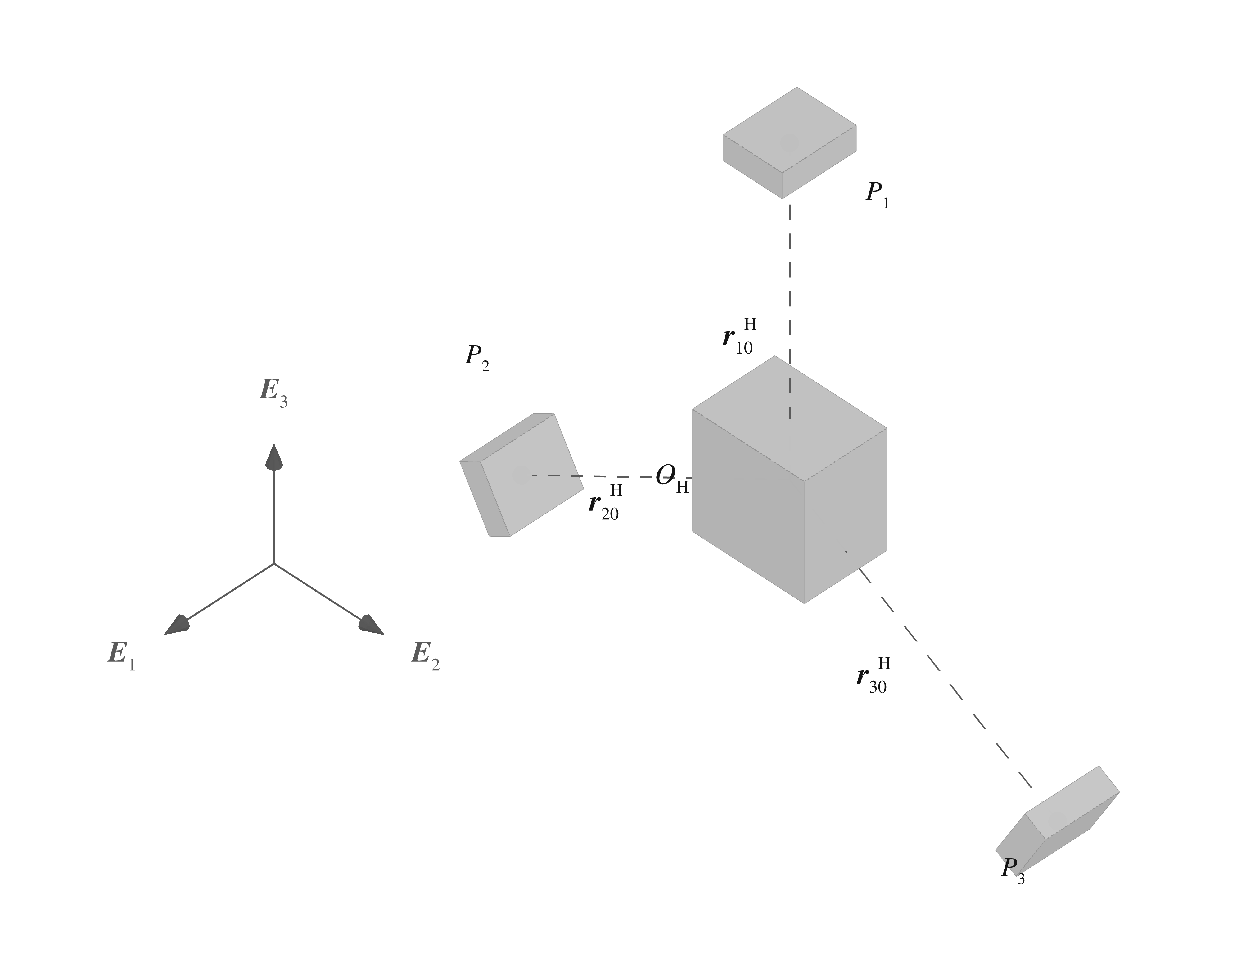
\includegraphics[width=.96\linewidth,height=.40\textheight,keepaspectratio]{figures/tecplot/concept_cubo-brazos.pdf}
\caption[Vínculo rígido entre el cubo y las raíces]{Brazos nominales $\vct r_{b0}^H$ desde el origen del cubo hasta las tres raíces $P_b$. Las líneas discontinuas distinguen estas relaciones geométricas de los volúmenes ilustrativos. Las separaciones son esquemáticas y no indican elementos flexibles adicionales.}\label{fig:cubo-brazos}
\end{figure}

Sea $\vct r_{s0}$ el brazo constante expresado en $\mathcal F_H$ y
$\ten Q_H={}^{N}\ten Q_H$ la orientación actual del cubo. La relación exacta
de posiciones es
\begin{equation}
 \vct x_s=\vct x_H+\ten Q_H\vct r_{s0}.
 \label{eq:fe-rigido-exacto}
\end{equation}
Para un vínculo soldado, la orientación de la raíz difiere de la del cubo
solo por una rotación de montaje constante. Si se permite una articulación
de paso, debe introducirse otra coordenada relativa; no se describe con el
vínculo soldado utilizado aquí.

Al variar \eqref{eq:fe-rigido-exacto}, expresando las rotaciones incrementales
en el mismo sistema de referencia $N$ y definiendo $\vct r_s=\ten Q_H\vct r_{s0}$, se obtiene
\begin{equation}
 \delta\vct u_s=\delta\vct u_H+
 \delta\vct\theta_H\times\vct r_s,
 \qquad \delta\vct\theta_s=\delta\vct\theta_H.
 \label{eq:desplazamiento-raiz}
\end{equation}
Por tanto,
\begin{equation}
 \delta\vct q_s=\ten B_s\delta\vct q_H,
 \qquad
 \ten B_s=\begin{bmatrix}\Id&-\sk{r_s}\\0&\Id\end{bmatrix}.
 \label{eq:compatibilidad-incremental}
\end{equation}
El brazo produce el desplazamiento de la raíz asociado a la rotación del
cubo; suprimirlo conserva solo una parte de la compatibilidad. La igualdad de
rotaciones incrementales presupone componentes comunes, no igualdad de
ángulos de Euler definidos en bases diferentes.

La suma vectorial de la figura~\ref{fig:vinculo-raiz} muestra por qué las traslaciones de una raíz y del punto maestro no son, en general, iguales. Incluso si el cubo no se traslada, su pequeña rotación desplaza una raíz situada a una distancia finita del eje. El término $\delta\vct\theta_H\times\vct r_s$ representa ese desplazamiento compatible, no una deformación del brazo.
\begin{figure}[htbp]
\centering
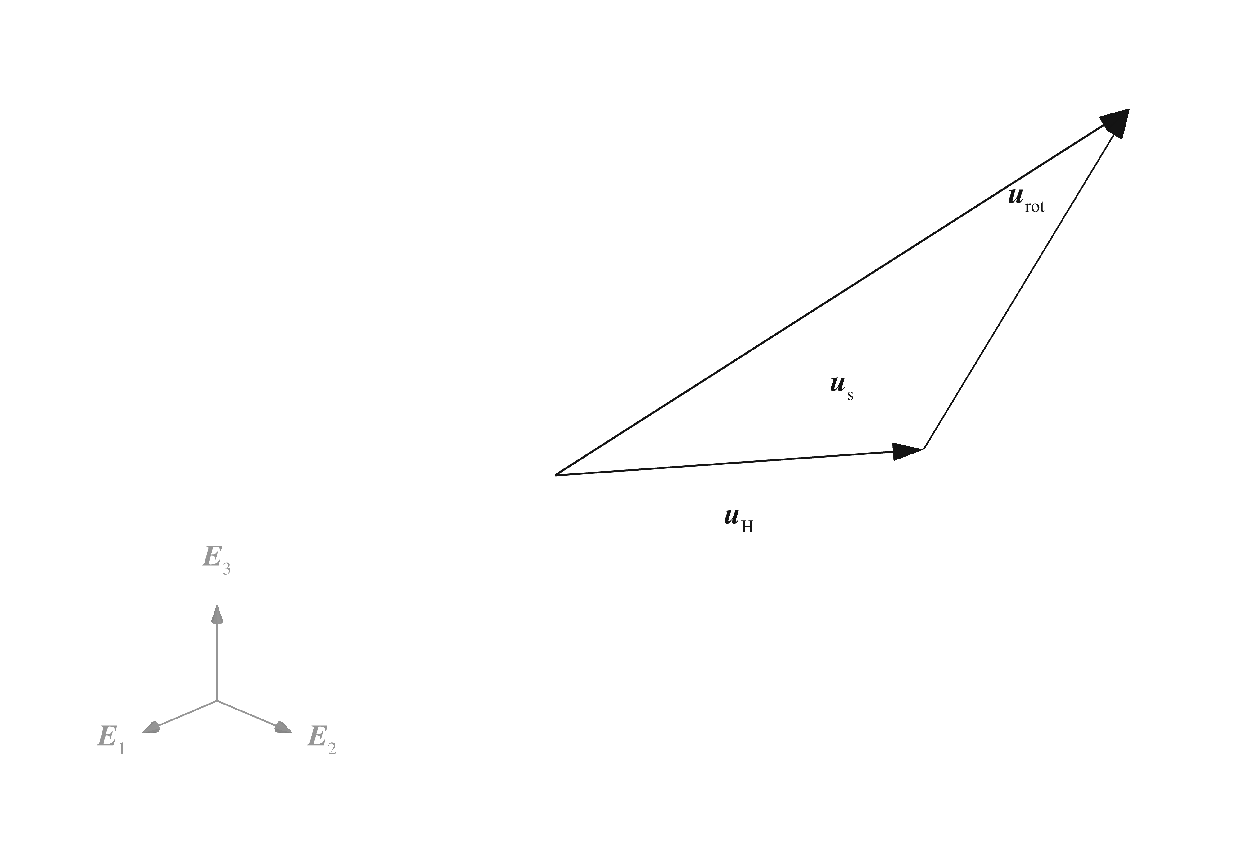
\includegraphics[width=.96\linewidth,height=.40\textheight,keepaspectratio]{figures/tecplot/concept_vinculo-raiz.pdf}
\caption[Desplazamiento compatible de una raíz]{Compatibilidad incremental de una raíz: $\vct u_s=\vct u_H+\vct u_{rot}$, donde $\vct u_{rot}=\vct\theta_H\times\vct r$. La suma se representa mediante flechas consecutivas y la flecha directa cierra el desplazamiento total. El punto intermedio corresponde solamente a la traslación común del cubo.}\label{fig:vinculo-raiz}
\end{figure}

\subsection{Restricciones dependientes del tiempo}

En el movimiento nominal de giro prescrito, los brazos expresados en $N$
varían aunque sean constantes en $H$. Para eje fijo,
\begin{equation}
 \dot{\vct r}_s=\sk{\Omega}\vct r_s,\qquad
 \ddot{\vct r}_s=\sk{\Omega}^{2}\vct r_s.
\end{equation}
Estas derivadas ocupan el bloque superior derecho de $\dot{\ten B}_s$ y
$\ddot{\ten B}_s$, con el mismo signo negativo. Si se reúnen los vínculos en
$\delta\vct q=\ten T(t)\vct z$, las velocidades y aceleraciones son
\begin{align}
 \delta\dot{\vct q}&=\ten T\dot{\vct z}+\dot{\ten T}\vct z,\\
 \delta\ddot{\vct q}&=\ten T\ddot{\vct z}
 +2\dot{\ten T}\dot{\vct z}+\ddot{\ten T}\vct z.
\end{align}
Sustituirlas en
$\ten M\delta\ddot{\vct q}+\ten D\delta\dot{\vct q}
+\ten K\delta\vct q=\delta\vct f$
y proyectar mediante $\ten T^{\tr}$ proporciona
\begin{align}
 \ten M_r&=\ten T^{\tr}\ten M\ten T,\\
 \ten D_r&=\ten T^{\tr}(\ten D\ten T+2\ten M\dot{\ten T}),\\
 \ten K_r&=\ten T^{\tr}(\ten K\ten T+\ten D\dot{\ten T}
 +\ten M\ddot{\ten T}),\\
 \vct f_r&=\ten T^{\tr}\delta\vct f.
 \label{eq:fe-reduccion-temporal}
\end{align}
Las reacciones ideales desaparecen de la ecuación proyectada porque no
realizan trabajo virtual sobre movimientos admisibles. Esta eliminación es
exacta dentro de las restricciones linealizadas y no equivale a truncar modos.
Una congruencia estática basta únicamente cuando $\dot{\ten T}=0$ y
$\ddot{\ten T}=0$. Elegir un azimut de evaluación no anula esas derivadas.

Los empotramientos y movimientos impuestos de la base $\mathcal F_B$ se
tratan asimismo como condiciones cinemáticas. Para una condición no homogénea
se escribe $\delta\vct q=\ten T\vct z+\vct q_p(t)$, y sus derivadas producen
la carga equivalente correspondiente. Así quedan separados los grados de
libertad estructurales, las coordenadas eliminadas por compatibilidad y los
movimientos prescritos. Esta separación es la base para introducir, en el
capítulo siguiente, el estado de operación y las ecuaciones de sus perturbaciones.

\section{Conexión elástica entre la góndola y el rotor}
La unión entre la góndola y el cubo transmite acciones que dependen de su movimiento relativo. Para pequeñas perturbaciones, sean $\vct u_G,\vct\theta_G$ y $\vct u_H,\vct\theta_H$ las traslaciones y rotaciones de los dos puntos de referencia, expresadas en una base común. El vector $\vct d$ une esos puntos en el estado alrededor del cual se linealiza. La deformación relativa se escribe
\begin{equation}
 \vct\Delta_d=
 \begin{bmatrix}
 \vct u_H-\vct u_G-\vct\theta_G\times\vct d\\
 \vct\theta_H-\vct\theta_G
 \end{bmatrix}
 =\mathsf B_d\vct q.
 \label{eq:conexion-elastica}
\end{equation}
El término $\vct\theta_G\times\vct d$ es el desplazamiento que tendría el punto del cubo si siguiera rígidamente la perturbación de la góndola. Restarlo permite medir únicamente el movimiento relativo que deforma la conexión. En particular, un movimiento de cuerpo rígido común a ambos componentes produce $\vct\Delta_d=\vct0$.

La figura~\ref{fig:conexion-elastica} representa las acciones de la conexión mediante un resorte y un amortiguador equivalentes. Estos símbolos sintetizan las relaciones entre las seis componentes relativas, no solo una traslación axial.

\begin{figure}[htbp]
\centering
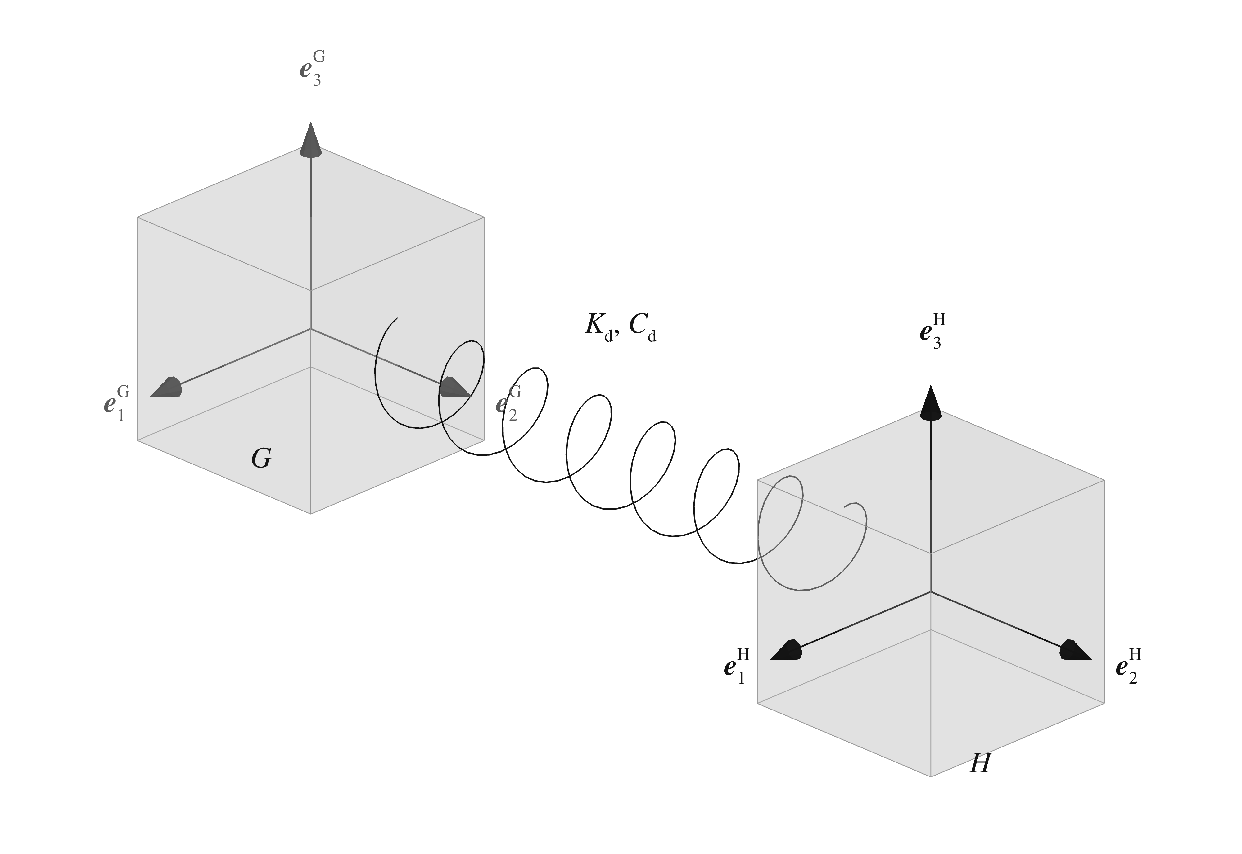
\includegraphics[width=.96\linewidth,height=.40\textheight,keepaspectratio]{figures/tecplot/concept_conexion-elastica.pdf}
\caption[Conexión elástica entre góndola y rotor]{Conexión elástica entre los sistemas de la góndola y el cubo. El resorte representa de forma simbólica los operadores generalizados de rigidez $K_d$ y disipación $C_d$. No implica un único grado de libertad ni fija la geometría de un cojinete comercial.}\label{fig:conexion-elastica}
\end{figure}

Con matrices de rigidez y amortiguamiento de conexión $\mathsf k_d$ y $\mathsf c_d$, las acciones conjugadas a $\vct\Delta_d$ son $\mathsf k_d\vct\Delta_d$ y $\mathsf c_d\dot{\vct\Delta}_d$. Para una matriz $\mathsf B_d$ constante, sus contribuciones al sistema son
\begin{equation}
 \mathsf K_d=\mathsf B_d^\tr\mathsf k_d\mathsf B_d,\qquad
 \mathsf C_d^{\,\mathrm{unión}}=\mathsf B_d^\tr\mathsf c_d\mathsf B_d.
\end{equation}
Si la base elegida hace que $\mathsf B_d$ dependa del tiempo, se conserva
$\dot{\vct\Delta}_d=\mathsf B_d\dot{\vct q}+\dot{\mathsf B}_d\vct q$.
La rigidez torsional de la conexión actúa sobre la desviación angular respecto del giro nominal. Una rigidez positiva produce una oscilación torsional elástica; no constituye un modo de cuerpo rígido.


\chapter{Ecuaciones de movimiento y análisis de vibraciones}
\label{ch:operacion}
\section{Movimiento impuesto y coordenadas desconocidas}
La función $\psi(t)=\psi_0+\Omega t$ describe una operación prescrita: su evolución se proporciona al modelo y no se obtiene resolviendo una ecuación de balance para el accionamiento. El par necesario para mantenerla puede ser una reacción del sistema idealizado. Por consiguiente, no se supone que el rotor gire libremente con momento angular constante. Velocidad angular impuesta y momento angular conservado son condiciones físicas distintas.

Una vez fijado ese movimiento, las coordenadas estructurales independientes se reúnen en $\vct q$. Incluyen desplazamientos y rotaciones de perturbación compatibles con los vínculos, mientras que $\psi$ es un dato. En la representación con conexión elástica se prescribe la rotación nominal del accionamiento y se conserva la torsión relativa del cubo como incógnita. Su ángulo total puede diferir de $\psi$ por una pequeña perturbación, determinada por la rigidez de la conexión y por las acciones del sistema. El caso de velocidad instantánea del cubo impuesta exactamente se obtiene restringiendo esa coordenada relativa.

En lo que sigue se estudia primero un estado estacionario relativo, para el cual los coeficientes expresados en las coordenadas elegidas no dependen explícitamente del tiempo. Esta hipótesis no se deduce solamente de $\Omega=\mathrm{constante}$. La gravedad sobre una pala giratoria, la interacción con una torre no giratoria o una carga no uniforme pueden producir coeficientes o fuerzas periódicos. El caso periódico se distingue al final del capítulo.

\section{Descomposición de la energía cinética}
\subsection{Grado en las velocidades generalizadas}
La cinemática de un sistema con movimiento impuesto permite que una partícula tenga velocidad distinta de cero aun cuando $\dot{\vct q}=\vct0$. Por ello, la energía cinética no es necesariamente una forma puramente cuadrática homogénea en $\dot{\vct q}$. Siguiendo la descomposición de sistemas no naturales expuesta por Meirovitch \cite[sección 4.1]{meirovitch}, se escribe
\begin{align}
 T(\vct q,\dot{\vct q})&=T_2+T_1+T_0,\\
 T_2&=\tfrac12\dot{\vct q}^{\tr}\mathsf M(\vct q)\dot{\vct q},\\
 T_1&=\dot{\vct q}^{\tr}\vct a(\vct q),\qquad
 T_0=T(\vct q,\vct0;\Omega).
 \label{eq:Tdecomp}
\end{align}
El subíndice indica el grado respecto de las velocidades generalizadas: dos, uno o cero. No indica el orden de una expansión en amplitud de desplazamiento. En particular, $T_0$ puede depender de $\vct q$ y no es una constante simplemente por llevar subíndice cero. El vector $\vct a$ de esta sección es el coeficiente de $T_1$, no la aceleración de una partícula; su argumento aclara el uso local del símbolo.

Si $V(\vct q)$ contiene las contribuciones con potencial de posición, se define el potencial efectivo o dinámico
\begin{equation}
 U_{\rm eff}(\vct q)=V(\vct q)-T_0(\vct q).
 \label{eq:Ueff}
\end{equation}
La función $T_0$ sigue siendo parte de la energía cinética física. Su signo negativo en $U_{\rm eff}$ procede de reorganizar el lagrangiano $L=T-V$ después de prescribir el movimiento, y no de convertir toda la dinámica en un problema conservativo. El accionamiento puede intercambiar energía con la estructura; las cargas aerodinámicas y la disipación se introducen por separado.

\subsection{Contribución nominal de una distribución de masa}
Considérese un cuerpo rígido, o una sección por unidad de longitud, en un sistema de referencia cuyo eje gira uniformemente. Sea $\vct y_C$ la posición de su centro de masa respecto al origen del eje y $Q$ su orientación relativa a ese sistema de referencia. Todas las componentes de esta subsección se expresan en él. Para un cuerpo de masa $m$ e inercia centroidal $J_C$ expresada en la base corporal,
\begin{equation}
 T_0=\tfrac12m\|W\vct y_C\|^2
 +\tfrac12\vct\Omega^{\tr}QJ_CQ^{\tr}\vct\Omega,
 \qquad W=[\vct\Omega]_\times.
 \label{eq:T0rigid}
\end{equation}
El primer término corresponde al desplazamiento orbital del centro de masa; el segundo, a la rotación de la distribución alrededor de su centro. Para una sección se sustituyen $m,J_C$ por $\mu,j_C$ y se integra sobre la longitud. El centro $\vct y_C$ incluye el brazo de conexión de la raíz, la posición longitudinal y la excentricidad de masa. Omitir el término orbital pierde gran parte de la contribución nominal de una pala al rotor.

El potencial asociado a esta contribución cinemática se puede escribir $V_\Omega=-T_0$. Para una masa puntual en $\vct y$,
\begin{equation}
 V_\Omega=-\tfrac12m\|W\vct y\|^2,
 \qquad -\frac{\partial V_\Omega}{\partial\vct y}
 =-mW^2\vct y.
\end{equation}
Este último vector es la carga inercial equivalente que aparece al formular el balance en el sistema de referencia giratorio. En cambio, la aceleración absoluta del punto fijo en ese sistema de referencia es $W^2\vct y$, dirigida hacia el eje. Son términos de signos opuestos ubicados en lados distintos del balance. El hecho de que la aceleración centrípeta cambie de dirección durante el giro no basta para clasificarla como una fuerza no conservativa. La existencia de $V_\Omega$ aquí depende de la velocidad de giro prescrita constante y de la descripción adoptada; no debe extenderse sin derivación a movimientos impuestos arbitrarios.

En una pala deformable, el giro puede generar esfuerzo axial y modificar la rigidez tangente. La contribución geométrica debida a ese esfuerzo y la derivada de $-T_0$ deben obtenerse a partir del mismo balance de equilibrio. Sumar una rigidez de pretensión aproximada a un hessiano que ya contiene el mismo efecto produce doble contabilización.

\section{Equilibrio relativo y movimiento sincrónico}
Un estado $\vct q_0$ constante en coordenadas apropiadas satisface
\begin{equation}
 \nabla U_{\rm eff}(\vct q_0)=\vct Q_0,
 \qquad \vct Q_0=\vct Q_{\rm nc}(\vct q_0,\vct0),
 \label{eq:equilibrio}
\end{equation}
donde $\vct Q_{\rm nc}$ reúne cargas generalizadas que no se han incluido en $V$. Esta igualdad caracteriza un equilibrio relativo, no el reposo absoluto de todas las partículas. Las partículas del rotor continúan describiendo el movimiento nominal y poseen velocidad y aceleración. La deformación que permanece fija en el sistema de referencia del rotor se transporta sincrónicamente con él.

Conviene separar tres objetos: la geometría material de referencia $\mathcal B_0$, la trayectoria nominal prescrita y el estado de operación deformado $\vct q_0$. El último depende de $\Omega$, cargas, rigideces y restricciones. No es necesariamente cero ni coincide con la geometría descargada. Una perturbación $\vct\eta(t)$ produce
\begin{equation}
 \vct q(t)=\vct q_0+\vct\eta(t).
\end{equation}
El estado de operación es la base de la linealización; las vibraciones se describen mediante $\vct\eta$. La palabra sincrónico se utiliza aquí para el transporte de la configuración relativa con el giro nominal. No implica que cualquier frecuencia propia sea igual a $\Omega$.

\subsection{Ejemplo elemental de equilibrio en un sistema de referencia giratorio}
Una masa $m$ se desplaza radialmente en una guía que gira a velocidad impuesta $\Omega$ y se une al eje mediante un resorte de rigidez $k$ y longitud natural $\ell$. Su coordenada radial es $r$. El ejemplo no representa una pala: permite distinguir movimiento y perturbación sin introducir matrices. Se tiene
\begin{equation}
 T=\tfrac12m\dot r^2+\tfrac12m\Omega^2r^2,
 \quad V=\tfrac12k(r-\ell)^2,
 \quad U_{\rm eff}=\tfrac12k(r-\ell)^2-\tfrac12m\Omega^2r^2.
\end{equation}
La ecuación radial y el equilibrio, cuando $k>m\Omega^2$, son
\begin{equation}
 m\ddot r+(k-m\Omega^2)r=k\ell,
 \qquad r_0=\frac{k\ell}{k-m\Omega^2}.
\end{equation}
Aunque $r_0$ es constante, la masa describe una circunferencia en el sistema de referencia newtoniano. Con $r=r_0+\eta$, la perturbación cumple $m\ddot\eta+(k-m\Omega^2)\eta=0$. La reacción transversal de la guía y el accionamiento hacen posible mantener el giro impuesto. Este ejemplo ilustra el potencial efectivo y no implica que el giro reduzca todas las frecuencias de una estructura: una pala incorpora también flexión, tensiones de operación y acoplamientos ausentes aquí.

La figura~\ref{fig:guia} muestra la guía y la trayectoria circular en una vista espacial: una coordenada radial constante es compatible con la rotación prescrita del conjunto.

\begin{figure}[htbp]
\centering
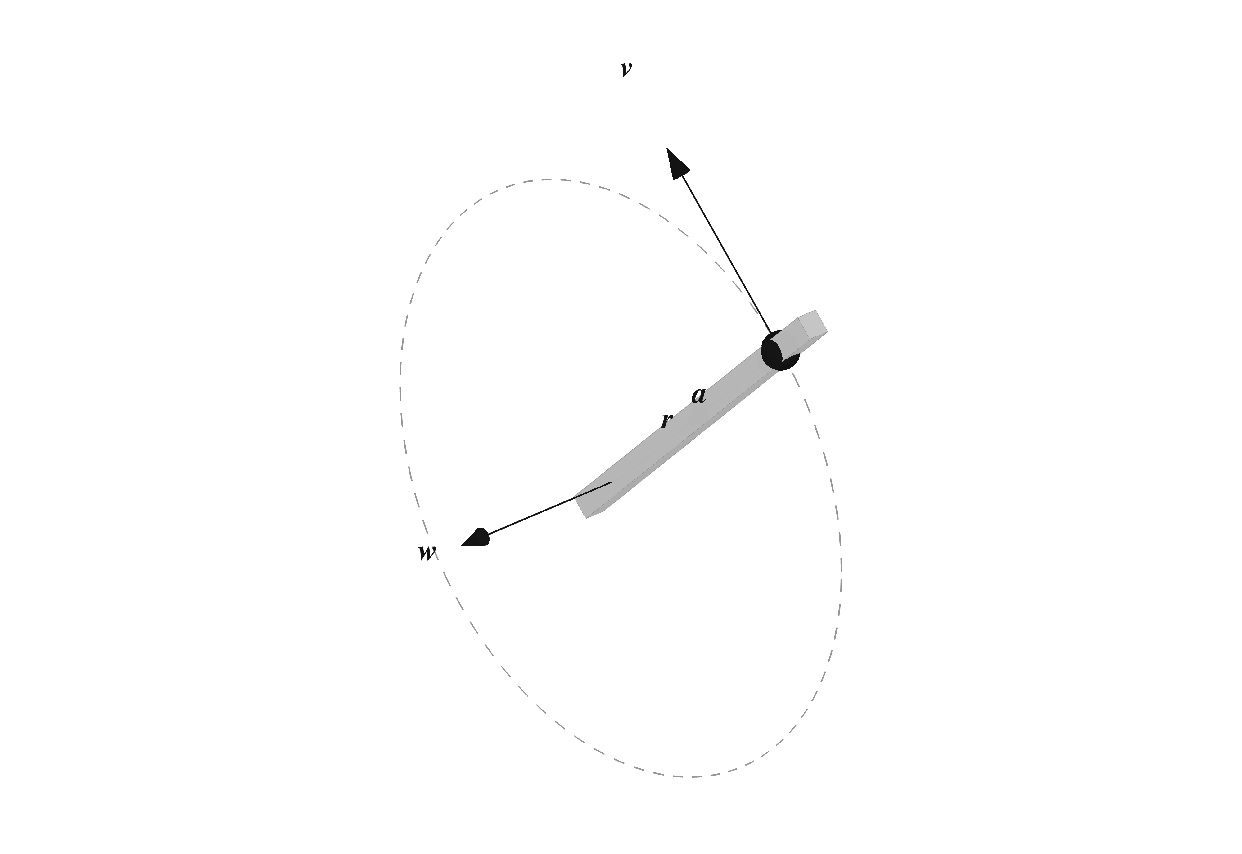
\includegraphics[width=.96\linewidth,height=.40\textheight,keepaspectratio]{figures/tecplot/concept_guia.pdf}
\caption[Equilibrio relativo en una guía giratoria]{Equilibrio relativo de un punto en una guía giratoria. La distancia radial constante es compatible con velocidad tangencial y aceleración centrípeta en el sistema inercial. La trayectoria discontinua y la guía con espesor distinguen el movimiento absoluto de la coordenada relativa.}\label{fig:guia}
\end{figure}

\section{Linealización alrededor del equilibrio de operación}
La linealización alrededor del equilibrio, presentada por Meirovitch en un paso distinto de la descomposición anterior \cite[sección 4.4]{meirovitch}, se obtiene reteniendo términos de grado total dos en el lagrangiano perturbado. Se definen
\begin{equation}
 \mathsf M_0=\mathsf M(\vct q_0),\quad
 A_{ij}=\left.\frac{\partial a_i}{\partial q_j}\right|_{\vct q_0},\quad
 \mathsf K_U=\left.\nabla^2 U_{\rm eff}\right|_{\vct q_0}.
\end{equation}
El término $\dot{\vct\eta}^{\tr}\vct a(\vct q_0)$ es una derivada temporal total si $\vct a(\vct q_0)$ es constante, y no altera las ecuaciones. Una vez balanceados los términos lineales por el equilibrio, la parte relevante de segundo grado es
\begin{equation}
 L^{(2)}=\tfrac12\dot{\vct\eta}^{\tr}\mathsf M_0\dot{\vct\eta}
 +\dot{\vct\eta}^{\tr}A\vct\eta
 -\tfrac12\vct\eta^{\tr}\mathsf K_U\vct\eta.
\end{equation}
El producto de la variación de $\mathsf M$ con dos velocidades perturbadas sería de tercer grado; por ello se evalúa la masa en $\vct q_0$. Aplicando las ecuaciones de Lagrange a la parte conservativa se obtiene
\begin{equation}
 \mathsf M_0\ddot{\vct\eta}
 +\underbrace{(A-A^{\tr})}_{\mathsf G}\dot{\vct\eta}
 +\mathsf K_U\vct\eta=\delta\vct Q_{\rm nc}.
 \label{eq:linearG}
\end{equation}
Así aparece la matriz giroscópica $\mathsf G$, con $\mathsf G^{\tr}=-\mathsf G$. No se postula su forma únicamente a partir de un momento angular nominal. El término de velocidad realiza potencia nula:
\begin{equation}
 \dot{\vct\eta}^{\tr}\mathsf G\dot{\vct\eta}=0.
\end{equation}
Puede intercambiar energía entre componentes del movimiento sin disiparla directamente. No es un amortiguamiento viscoso positivo ni la derivada de un potencial de posición.

\section{Deducción de la matriz giroscópica de un cuerpo rígido}
\subsection{Parte traslacional y parte angular}
Se consideran pequeñas coordenadas relativas $\vct z=[\vct u^{\tr},\vct\theta^{\tr}]^{\tr}$ en un sistema de referencia que gira uniformemente, con $\vct\theta$ parametrizada por la representación exponencial. Se emplea una parametrización incremental centrada en el estado de linealización: en él $\vct z=0$, y su orientación se incorpora previamente a las propiedades. Sea $\vct c$ el vector desde el punto de referencia hasta el centro de masa, y $J$ la matriz de inercia centroidal en esa misma base. Defínanse
\begin{equation}
 B=\begin{bmatrix}\Id&-[\vct c]_\times\end{bmatrix},\qquad
 E_\theta=\begin{bmatrix}0&\Id\end{bmatrix},\qquad W=[\vct\Omega]_\times.
\end{equation}
La perturbación lineal del centro es $B\vct z$ y su velocidad relativa lineal $B\dot{\vct z}$. Al expandir la energía traslacional, el término mixto relevante es $m(B\dot{\vct z})^{\tr}W(B\vct z)$; su parte antisimétrica produce $2mB^{\tr}WB$.

La rotación requiere conservar la precisión de segundo orden: la velocidad angular relativa no puede reemplazarse por $\dot{\vct\theta}$ antes de formar todos los términos mixtos. En efecto,
\begin{equation}
 \vct\omega=\vct\Omega+\dot{\vct\theta}
 +\tfrac12[\vct\theta]_\times\dot{\vct\theta}+O(3),
 \quad QJQ^{\tr}=J+[\vct\theta]_\times J-J[\vct\theta]_\times+O(2).
\end{equation}
Aquí $O(3)$ cuenta grado total en amplitudes y velocidades perturbadas; el término nominal $\vct\Omega$ no es pequeño. Al sustituir en $\tfrac12\vct\omega^{\tr}QJQ^{\tr}\vct\omega$, los términos mixtos pueden reunirse como
\begin{equation}
 \dot{\vct\theta}^{\tr}A_\theta\vct\theta,
 \qquad A_\theta=JW-\tfrac12[J\vct\Omega]_\times.
\end{equation}
Su parte antisimétrica da
\begin{equation}
 \mathsf G_\theta=JW+WJ-[J\vct\Omega]_\times.
\end{equation}
Por tanto, la matriz completa de seis coordenadas es
\begin{equation}
 \boxed{\mathsf G_6=2mB^{\tr}WB+
 E_\theta^{\tr}\bigl(JW+WJ-[J\vct\Omega]_\times\bigr)E_\theta.}
 \label{eq:G6}
\end{equation}
Cada bloque se obtiene de la misma cinemática y de la misma elección de coordenadas. Si se usan componentes angulares corporales o se linealizan directamente ecuaciones de Euler, la forma intermedia puede cambiar; se debe transformar también la cinemática para comparar matrices. No basta con sustituir $\mathsf G_\theta$ por $-[J\vct\Omega]_\times$ conservando sin cambios las restantes definiciones.

\subsection{Caso centroidal y ejes principales}
Para $\vct c=\vct0$, $J=\diag(J_1,J_2,J_3)$ y $\vct\Omega=(\Omega,0,0)^{\tr}$,
\begin{equation}
 \mathsf G_6=\begin{bmatrix}2mW&0\\0&\mathsf G_\theta\end{bmatrix},
 \qquad
 \mathsf G_\theta=\Omega
 \begin{bmatrix}0&0&0\\0&0&-(J_2+J_3-J_1)\\0&J_2+J_3-J_1&0\end{bmatrix}.
\end{equation}
La combinación de inercias es consecuencia de la parametrización relativa empleada. La nulidad de alguna combinación en una idealización geométrica no demuestra ausencia de todos los efectos de giro: permanecen contribuciones traslacionales, excentricidades, restricciones y términos dependientes de $\Omega^2$.

Para una viga se construye la expresión seccional $\mathsf G_s$ con $\mu,j_C,\vct c_m$ y se usa la interpolación cinemática del capítulo anterior:
\begin{equation}
 \mathsf G_e=\int_0^{L_e}N^{\tr}\mathsf G_sN\,\dd S.
\end{equation}
La orientación, el ensamblaje y las restricciones se aplican después con las mismas transformaciones que para masa y rigidez. Si un cambio de coordenadas depende del tiempo, sus derivadas también generan términos de transporte, como se mostró en la reducción temporal. No se deben añadir dos veces efectos que ya están representados por esas derivadas.

La figura~\ref{fig:acoplamiento-giroscopico} representa la acción de un bloque antisimétrico de dos componentes. Si $\vct w=(\dot\theta_2,\dot\theta_3)^\tr$ y $g_\theta=(J_2+J_3-J_1)\Omega$, el bloque angular anterior produce
\begin{equation}
 \vct h_g=
 \begin{bmatrix}0&-g_\theta\\g_\theta&0\end{bmatrix}\vct w,
 \qquad \vct w^\tr\vct h_g=0.
\end{equation}
En el esquema se representan las direcciones normalizadas $\widehat{\vct w}=\vct w/\|\vct w\|$ y $\widehat{\vct h}_g=\vct h_g/\|\vct h_g\|$, para vectores no nulos. Aquí $\vct h_g$ es el término inercial generalizado de ese bloque; no se introduce una acción externa adicional. Su ortogonalidad con la velocidad explica la potencia nula y no impide que cambien los modos del sistema acoplado.

\begin{figure}[htbp]
\centering
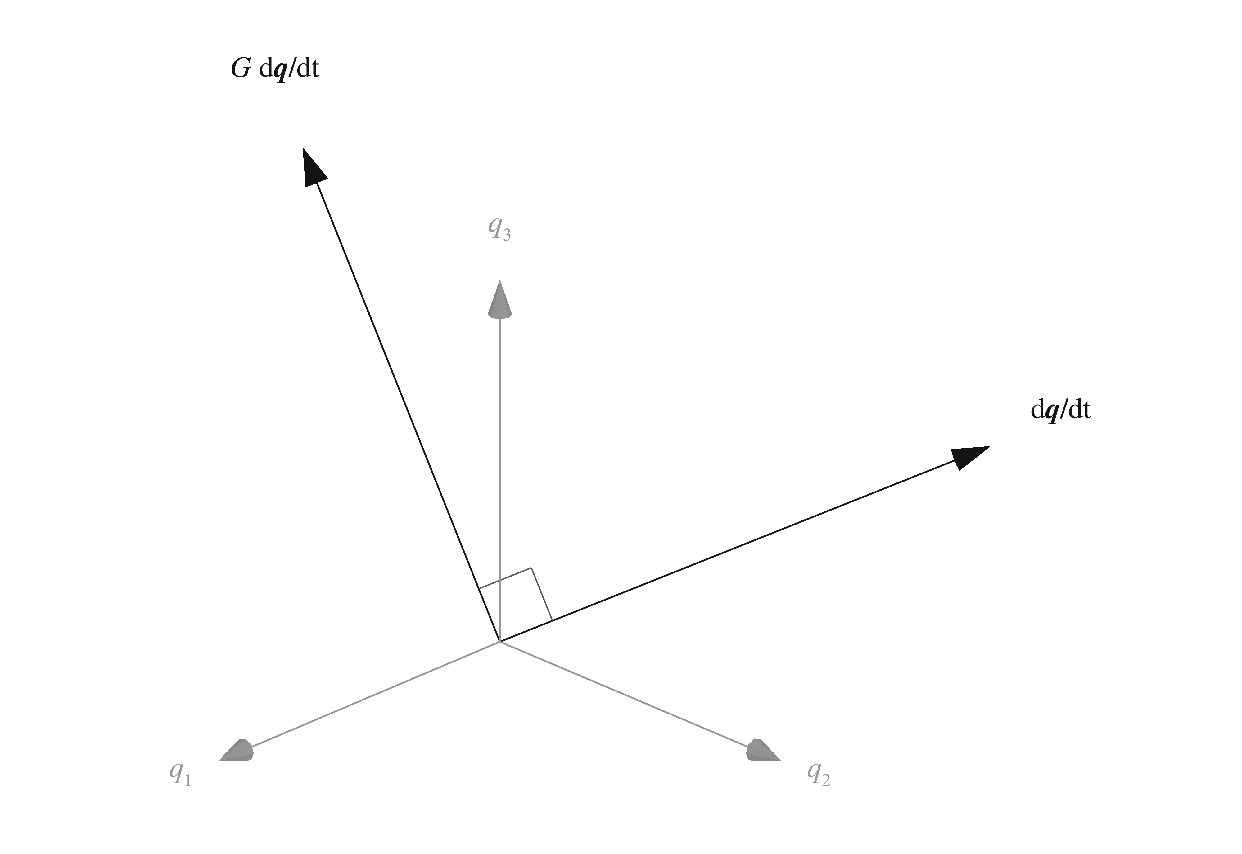
\includegraphics[width=.96\linewidth,height=.40\textheight,keepaspectratio]{figures/tecplot/concept_acoplamiento-giroscopico.pdf}
\caption[Antisimetría del acoplamiento giroscópico]{Representación geométrica de una contribución giroscópica antisimétrica. Los vectores $\dot{\vct q}$ y $G\dot{\vct q}$ son ortogonales, de modo que $\dot{\vct q}^{\tr}G\dot{\vct q}=0$. El triedro identifica coordenadas del espacio de perturbaciones; el dibujo ilustra esta identidad y no una forma modal calculada.}\label{fig:acoplamiento-giroscopico}
\end{figure}

\section{Cargas generalizadas y amortiguamiento}
Alrededor del estado de operación, una carga generalizada diferenciable puede escribirse
\begin{equation}
 \delta\vct Q_{\rm nc}=\mathsf Q_q\vct\eta+
 \mathsf Q_v\dot{\vct\eta}+\vct f(t).
\end{equation}
Con un amortiguamiento estructural separado $\mathsf C_d$, la ecuación resulta
\begin{equation}
 \mathsf M_0\ddot{\vct\eta}+\mathsf D\dot{\vct\eta}
 +\mathsf K\vct\eta=\vct f(t),\qquad
 \mathsf D=\mathsf G+\mathsf C_d-\mathsf Q_v,
 \quad\mathsf K=\mathsf K_U-\mathsf Q_q.
 \label{eq:finaldynamic}
\end{equation}
Una matriz $\mathsf K$ no simétrica puede proceder de cargas seguidoras. Sus coeficientes no se deducen de un hessiano simétrico de energía potencial ordinaria. Para una base traslacional impuesta, la carga equivalente aparece al sustituir el movimiento particular en el balance; en coordenadas relativas y bajo las hipótesis usuales de masa constante toma la forma $-\mathsf M_0\mathsf\Gamma\ddot{\vct u}_B$, con $\mathsf\Gamma$ definido por la cinemática de participación de la base. La carga de viento se incorpora mediante fuerzas distribuidas y momentos consistentes, transformados desde la base de evaluación aerodinámica a la estructural, manteniendo el sistema de referencia newtoniano definido en la cinemática.

La matriz $\mathsf Q_q$ representa la variación de la carga respecto de las coordenadas estructurales, mientras que $\mathsf Q_v$ representa su variación respecto de las velocidades. En una carga conservativa de posición, la tangente procede de un potencial y es simétrica bajo las hipótesis de regularidad. Para una carga seguidora, esa propiedad no está garantizada. Una matriz puede representar un operador lineal aunque la acción física correspondiente no sea conservativa: la existencia de un potencial es una propiedad adicional, no parte de la definición de operador.

La disipación viscosa simétrica puede expresarse mediante la función de Rayleigh $\mathcal R=\tfrac12\dot{\vct q}^{\tr}\mathsf C_d\dot{\vct q}$ y la fuerza $-\partial\mathcal R/\partial\dot{\vct q}$. Esta función describe la disipación, no una energía potencial almacenada. Por su parte, la matriz giroscópica procede de la energía cinética y realiza potencia instantánea nula. De esta manera, las contribuciones conservativas, disipativas y giroscópicas quedan diferenciadas por su origen y por su intervención en el balance de energía.

\subsection{Gravedad y acciones aerodinámicas}
La aceleración de gravedad es un vector fijo en el sistema inercial,
$\vct g=-g\vct E_3$, con $g>0$. Un cuerpo rígido recibe la fuerza $m\vct g$ aplicada en su centro de masa. Respecto de otro punto de referencia, esta fuerza produce además el momento $\vct c\times m\vct g$. En una viga, ambas contribuciones se obtienen integrando la masa y la excentricidad de cada sección. La transformación al sistema giratorio modifica sus componentes, aunque la dirección física de la gravedad permanezca constante.

Para introducir las acciones aerodinámicas se define primero la velocidad relativa del aire respecto de una partícula de la superficie:
\begin{equation}
 \vct v_{\mathrm{rel}}(\vct X,t)
 =\vct v_{\mathrm{aire}}(\vct x,t)-\vct v_{\mathrm{estructura}}(\vct X,t).
 \label{eq:velocidad-relativa-aire}
\end{equation}
Ambas velocidades se expresan en la misma base y se evalúan en la misma posición espacial. La velocidad estructural incluye el giro nominal, la traslación de la base y la perturbación elástica. Por tanto, una velocidad del viento constante no produce necesariamente una carga constante en los ejes de la pala.

Sean $\vct p_a$ y $\vct\ell_a$ la fuerza y el momento aerodinámicos por unidad de longitud, expresados respecto del punto de referencia de la sección. Si una fuerza actúa en un punto desplazado por $\vct a_a$ respecto de ese origen, el momento equivalente contiene $\vct a_a\times\vct p_a$, además del momento propio de la distribución de presiones. La carga nodal consistente es
\begin{equation}
 \vct f_{a,e}
 =\int_0^{L_e}N^\tr
 \begin{bmatrix}\vct p_a\\\vct\ell_a\end{bmatrix}\dd s.
 \label{eq:viento-consistente}
\end{equation}
La igualdad de trabajo virtual determina la transferencia entre las acciones distribuidas y las coordenadas estructurales. La ley aerodinámica que proporciona $\vct p_a$ y $\vct\ell_a$ es un dato adicional del modelo de cargas; puede proceder de una distribución prescrita o de un cálculo del flujo.

La figura~\ref{fig:carga-seccion} separa el punto de aplicación de la fuerza de su representación equivalente en la línea estructural. Si $\vct\ell_A$ es el momento propio referido a $A$, el momento en $O_s$ es $\vct\ell_a=\vct\ell_A+\vct a_a\times\vct p_a$; no deben aplicarse simultáneamente las dos representaciones.

\begin{figure}[htbp]
\centering
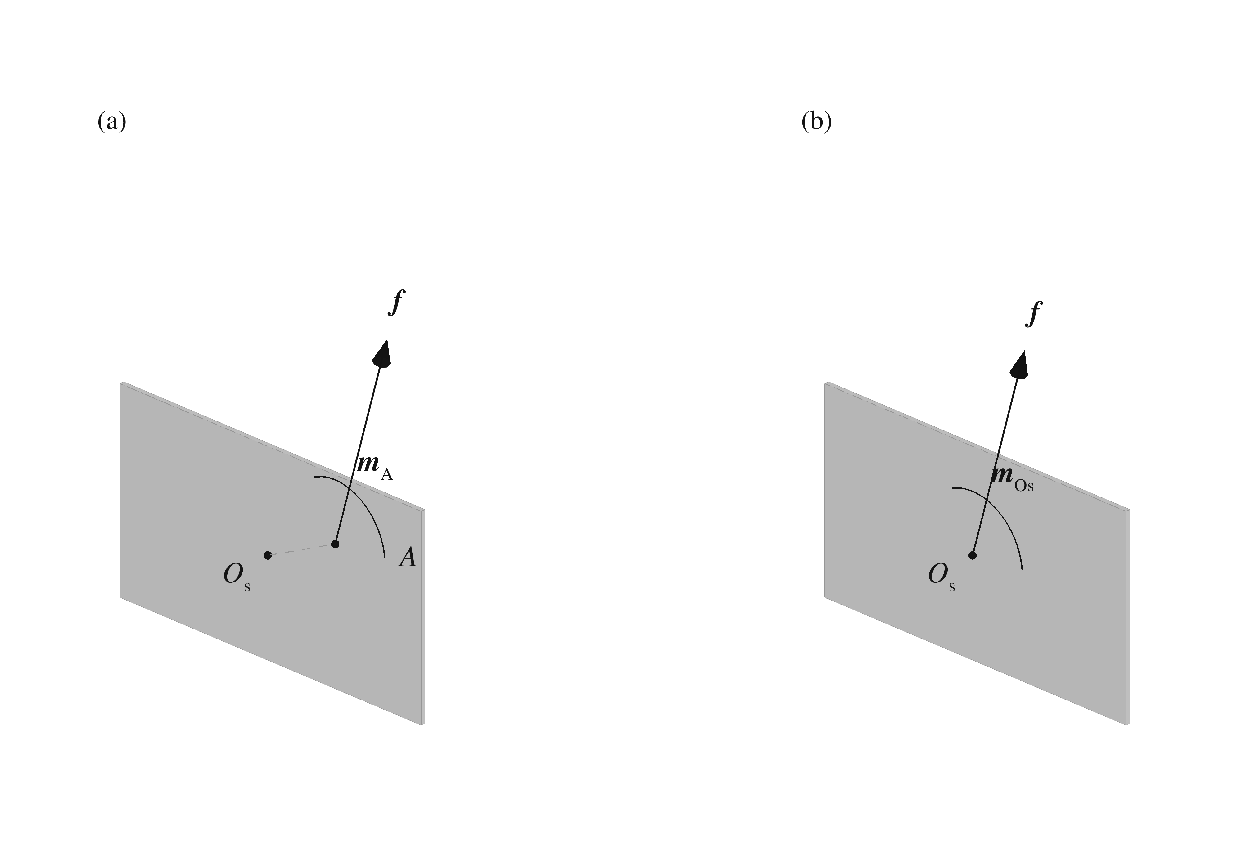
\includegraphics[width=.96\linewidth,height=.40\textheight,keepaspectratio]{figures/tecplot/concept_carga-seccion.pdf}
\caption[Transferencia de cargas aerodinámicas]{Transporte de una resultante de sección: (a) fuerza y momento aplicados en un punto $A$ y (b) representación equivalente respecto de $O_s$. La fuerza se conserva y el momento cambia según $\vct m_{O_s}=\vct m_A+\vct r_A\times\vct f$. Los arcos señalan la dirección de los momentos; sus radios son ilustrativos.}\label{fig:carga-seccion}
\end{figure}

Al linealizar, la variación aerodinámica se separa en
\begin{equation}
 \delta\vct f_a
 =\mathsf F_{a,q}\vct\eta+\mathsf F_{a,v}\dot{\vct\eta}
  +\delta\vct f_{a,\mathrm{imp}}(t).
\end{equation}
El último término corresponde a la variación impuesta del flujo; los dos primeros recogen la dependencia de la fuerza respecto del movimiento estructural. Sus contribuciones a la rigidez y al coeficiente de velocidad son $-\mathsf F_{a,q}$ y $-\mathsf F_{a,v}$. En particular, la dirección de una carga seguidora cambia con la orientación del componente. La derivada de esa dirección debe conservarse y puede producir una tangente no simétrica. La dependencia de la carga respecto del movimiento se evalúa con la misma ley utilizada para determinar el estado de operación.

\subsection{Excitación sísmica y recuperación del movimiento absoluto}
La traslación impuesta del terreno se denota $\vct u_B(t)$ y su aceleración $\vct a_B(t)=\ddot{\vct u}_B(t)$. Para construir la carga equivalente se parte de las coordenadas completas, incluidas las de apoyo, y se escribe
\begin{equation}
 \vct q_{\mathrm{abs}}=\mathsf T(t)\vct z+\mathsf\Gamma_f\vct u_B.
 \label{eq:movimiento-base}
\end{equation}
El vector $\vct z$ reúne las coordenadas independientes relativas y la matriz $\mathsf T$ impone la compatibilidad. La matriz $\mathsf\Gamma_f$ distribuye una traslación uniforme de la base: sus bloques traslacionales son identidades y sus bloques angulares son nulos cuando todas las componentes se expresan en ejes inerciales. Una descripción en ejes móviles requiere transformar también esta influencia y conservar sus derivadas.

Con $\mathsf\Gamma_f$ constante, la sustitución de \eqref{eq:movimiento-base} en las ecuaciones completas y la proyección sobre los movimientos admisibles producen la contribución
\begin{equation}
 \vct f_B=-\mathsf T^\tr\left(
 \mathsf M\mathsf\Gamma_f\ddot{\vct u}_B+
 \mathsf D\mathsf\Gamma_f\dot{\vct u}_B+
 \mathsf K\mathsf\Gamma_f\vct u_B\right).
 \label{eq:sismo-general}
\end{equation}
En esta ecuación, $\mathsf M,\mathsf D,\mathsf K$ son los coeficientes de las ecuaciones completas antes de eliminar los apoyos. Si las fuerzas elásticas y disipativas se definen respecto del movimiento relativo al terreno, o anulan la traslación rígida correspondiente, la expresión se reduce a
\begin{equation}
 \vct f_B=-\mathsf P_B\vct a_B,\qquad
 \mathsf P_B=\mathsf T^\tr\mathsf M\mathsf\Gamma_f.
 \label{eq:sismo-inercia}
\end{equation}
La matriz $\mathsf P_B$ conserva el acoplamiento de masa con las coordenadas prescritas. Una carga aerodinámica dependiente de la velocidad absoluta puede aportar términos adicionales asociados a $\dot{\vct u}_B$; estos se mantienen en la ley de carga.

La aceleración absoluta se reconstruye diferenciando la relación cinemática,
\begin{equation}
 \ddot{\vct q}_{\mathrm{abs}}
 =\mathsf T\ddot{\vct z}
  +2\dot{\mathsf T}\dot{\vct z}
  +\ddot{\mathsf T}\vct z
  +\mathsf\Gamma_f\vct a_B.
\end{equation}
Cuando $\vct q_{\mathrm{abs}}$ representa únicamente la perturbación, la aceleración total de una partícula se obtiene añadiendo la aceleración de su movimiento nominal. De esta forma se distinguen la aceleración relativa de vibración, la contribución sísmica y la aceleración asociada al giro.

\section{Frecuencias naturales y modos de vibración}
Para coeficientes constantes, las vibraciones libres de \eqref{eq:finaldynamic} se buscan como $\vct\eta=\vct\phi e^{\lambda t}$, lo que conduce al problema cuadrático \cite{tisseur}
\begin{equation}
 (\lambda^2\mathsf M_0+\lambda\mathsf D+\mathsf K)\vct\phi=\vct0.
\end{equation}
El autovector $\vct\phi$ describe una dirección de perturbación del estado $\vct q_0$; no determina por sí mismo ese equilibrio. Las matrices dependen de $\vct q_0$ y $\Omega$, por lo que cambiar el estado de operación cambia el problema modal. Cuando $\mathsf D=0$, $\mathsf M_0$ es positiva definida y $\mathsf K$ es simétrica, se recupera $\mathsf K\vct\phi_j=\omega_j^2\mathsf M_0\vct\phi_j$. En presencia de efectos giroscópicos, la formulación cuadrática es la forma general apropiada y los autovectores pueden ser complejos.

Existe una relación especial que conviene no confundir con lo anterior. En un problema estático lineal conservativo $\mathsf K\vct q_0=\vct f_0$, con $\mathsf K$ invertible y una base modal completa normalizada por masa, puede escribirse
\begin{equation}
 \vct q_0=\sum_j\vct\phi_j\frac{\vct\phi_j^{\tr}\vct f_0}{\omega_j^2},
 \qquad\vct\phi_i^{\tr}\mathsf M_0\vct\phi_j=\delta_{ij}.
\end{equation}
Es una expansión de una solución estática en una base, no una identidad entre equilibrio y modo. No se aplica directamente si hay modos rígidos de frecuencia cero, rigidez singular o un equilibrio no lineal dependiente de la deformación.

\section{Límite entre equilibrio relativo y régimen periódico}
Cuando las ecuaciones conservan una dependencia periódica del azimut, el estado de operación puede ser una trayectoria $\vct q_p(t)$ con período $2\pi/\Omega$ y no un vector constante. La perturbación se define entonces por $\vct q=\vct q_p+\vct\eta$ y satisface un sistema lineal de coeficientes periódicos. Su estabilidad se estudia mediante la evolución sobre un período, no interpretando sin más los autovalores de una matriz evaluada en un único azimut como frecuencias globales.

Una evaluación a azimut fijo es una aproximación local que debe identificarse como tal. Las transformaciones multípala pueden simplificar la periodicidad de un rotor simétrico \cite{bir}, pero no garantizan eliminarla bajo cargas o propiedades arbitrarias. Con esta separación quedan definidos los niveles del modelo: cinemática exacta de sección rígida, discretización estructural, estado de operación adoptado y dinámica lineal de sus perturbaciones. Cada nivel conserva sus hipótesis y su alcance sin atribuir al modelo lineal capacidades que pertenecen a una formulación no lineal o periódica más general.
\appendix

\chapter{Notación}
\small
\section{Entidades geométricas y sistemas de referencia}
\begin{longtable}{p{.24\textwidth}p{.69\textwidth}}
\toprule Símbolo & Significado \\\midrule\endhead
$\mathcal B$ & Cuerpo material: conjunto de partículas identificables.\\
$\mathcal B_0,\mathcal B_t$ & Configuraciones de referencia y actual.\\
$\vct X,\vct x$ & Posiciones material de referencia y espacial actual.\\
$\vct\chi$ & Movimiento que asigna $\vct x=\vct\chi(\vct X,t)$.\\
$\vct u$ & Desplazamiento; su referencia concreta se indica en cada representación.\\
$\mathcal F_A$ & Sistema de referencia con origen $O_A$ y base ortonormal dextrógira.\\
$N,B,G,H,P_b$ & Newtoniano, base, góndola, cubo y montaje de pala $b$.\\
${}^AQ_B$ & Cambio de componentes de la base $B$ a la base $A$.\\
$\overline{(\cdot)}$ & Cantidad nominal o sistema de referencia de movimiento prescrito.\\
$\psi,\Omega$ & Azimut prescrito y velocidad angular nominal constante.\\
$[\vct a]_\times$ & Matriz del producto vectorial: $[\vct a]_\times\vct b=\vct a\times\vct b$.\\
$\Grad,\grad$ & Derivadas espaciales respecto de coordenadas materiales y actuales, respectivamente.\\
$\ten F,J$ & Gradiente de deformación y su determinante.\\
$\ten C,\ten E$ & Tensor derecho de Cauchy--Green y deformación de Green--Lagrange.\\
$\ten R,\ten U,\ten V$ & Rotación polar y estiramientos derecho e izquierdo.\\
\bottomrule
\end{longtable}

\section{Vigas y propiedades físicas}
\begin{longtable}{p{.24\textwidth}p{.69\textwidth}}
\toprule Símbolo & Significado y unidades \\\midrule\endhead
$S,\xi_2,\xi_3$ & Coordenadas materiales de línea y sección, $\mathrm m$.\\
$\vct R,\vct r$ & Posición de la línea de referencia y posición actual de esa línea, $\mathrm m$.\\
$\vct D_i,\vct d_i$ & Directores de sección de referencia y actuales.\\
$\vct\gamma,\vct\kappa$ & Extensión/cortantes y cambio de curvatura/torsión, $1$ y $\mathrm{m^{-1}}$.\\
$\vct n,\vct m$ & Resultantes seccionales de fuerza y momento, $\mathrm N$ y $\mathrm{N\,m}$.\\
$A,\vct c_A$ & Área y centro de área relativo al origen seccional, $\mathrm{m^2}$ y $\mathrm m$.\\
$\ten S_A,\ten I_A$ & Tensores geométricos de segundo momento, $\mathrm{m^4}$.\\
$J_t$ & Constante torsional de Saint-Venant, $\mathrm{m^4}$.\\
$\rho_0,\mu,m$ & Densidad de referencia, masa por longitud y masa total, $\mathrm{kg/m^3}$, $\mathrm{kg/m}$ y $\mathrm{kg}$.\\
$\vct c_m$ & Vector de excentricidad del centro de masa seccional, $\mathrm m$.\\
$\ten j_C,\ten J_C$ & Inercia centroidal por longitud y total, $\mathrm{kg\,m}$ y $\mathrm{kg\,m^2}$.\\
$\mathsf M_s,\mathsf C_s$ & Matrices seccionales de masa y rigidez, con unidades diferentes entre bloques.\\
$E,G,\nu$ & Módulos de Young y cortante, y coeficiente de Poisson.\\
$A_{s2},A_{s3}$ & Áreas efectivas de cortante, $\mathrm{m^2}$.\\
\bottomrule
\end{longtable}

\section{Discretización y dinámica}
\begin{longtable}{p{.24\textwidth}p{.69\textwidth}}
\toprule Símbolo & Significado \\\midrule\endhead
$\vct q_e$ & Coordenadas de un elemento; doce antes de restricciones para la viga de dos nodos.\\
$N,B$ & Interpolación cinemática y relación discreta deformación--coordenadas.\\
$\mathsf M,\mathsf K$ & Matrices discretas de masa y rigidez; los índices especifican elemento, reducción o tangente.\\
$\mathsf G$ & Matriz antisimétrica de efectos giroscópicos en las coordenadas declaradas.\\
$\mathsf C_d,\mathsf D$ & Amortiguamiento estructural y coeficiente total de velocidades.\\
$\vct q_0,\vct\eta$ & Estado de equilibrio relativo y perturbación respecto de él.\\
$T_2,T_1,T_0$ & Partes de la energía cinética de grados dos, uno y cero en velocidades generalizadas.\\
$U_{\rm eff}$ & Potencial efectivo $V-T_0$ bajo las hipótesis de movimiento prescrito indicadas.\\
$\lambda,\vct\phi$ & Autovalor y autovector del problema de perturbaciones.\\
\bottomrule
\end{longtable}
Un punto sobre una cantidad indica derivada temporal manteniendo fijas las coordenadas materiales o relativas especificadas. Una prima en la cinemática de viga indica derivada respecto de $S$; en la interpolación normalizada debe aplicarse la regla de la cadena. El superíndice $\tr$ denota transposición, no derivada. Los índices $i,j$ son índices de componentes; $b$ identifica pala y $e$ elemento. Las matrices de seis o doce coordenadas se escriben por bloques para no confundirlas con tensores físicos tridimensionales.

Al pasar de un capítulo a otro, las mismas letras pueden representar la entidad geométrica y su matriz de componentes cuando la base ya está fijada. Las ecuaciones que mezclan sistemas de referencia incorporan explícitamente los cambios ${}^AQ_B$. Ninguna comparación entre matrices de masa, inercia o efectos de giro es válida sin comprobar antes origen, orientación, orden de coordenadas y unidades.
\normalsize

\begin{thebibliography}{99}
\addcontentsline{toc}{chapter}{Bibliografía}
\bibitem{holzapfel} Holzapfel, G. A. (2000). \emph{Nonlinear Solid Mechanics: A Continuum Approach for Engineering}. John Wiley \& Sons. ISBN 978-0-471-82319-3.
\bibitem{meirovitch} Meirovitch, L. (1997). \emph{Principles and Techniques of Vibrations}. Prentice Hall. Secciones 4.1 y 4.4, pp. 142--145 y 162--166: sistemas no naturales y linealización alrededor del equilibrio.
\bibitem{reddy} Reddy, J. N. (2006). \emph{An Introduction to the Finite Element Method}. Tercera edición, McGraw-Hill.
\bibitem{shabana} Shabana, A. A. (2013). \emph{Dynamics of Multibody Systems}. Cuarta edición, Cambridge University Press. \url{https://doi.org/10.1017/CBO9781107337213}.
\bibitem{bir} Bir, G. S. (2008). \emph{Multiblade Coordinate Transformation and Its Application to Wind Turbine Analysis}. NREL/CP-500-42553. \url{https://www.osti.gov/servlets/purl/922553}.
\bibitem{tisseur} Tisseur, F. y Meerbergen, K. (2001). The quadratic eigenvalue problem. \emph{SIAM Review}, 43(2), 235--286. \url{https://doi.org/10.1137/S0036144500381988}.
\bibitem{gebhardt2008} Gebhardt, C., Preidikman, S., Massa, J. C. y Weber, G. (2008). Comportamiento aerodinámico y aeroelástico de rotores de generadores eólicos de eje horizontal y de gran potencia. \emph{Mecánica Computacional}, 27, 519--539. \url{https://cimec.org.ar/ojs/index.php/mc/article/view/1435}.
\bibitem{simo1985} Simo, J. C. (1985). A finite strain beam formulation. The three-dimensional dynamic problem. Part I. \emph{Computer Methods in Applied Mechanics and Engineering}, 49(1), 55--70. \url{https://doi.org/10.1016/0045-7825(85)90050-7}.
\bibitem{wang2017} Wang, Q., Sprague, M. A., Jonkman, J., Johnson, N. y Jonkman, B. (2017). BeamDyn: A high-fidelity wind turbine blade solver in the FAST modular framework. \emph{Wind Energy}, 20(8), 1439--1462. \url{https://doi.org/10.1002/we.2101}.
\bibitem{faccio2019} Faccio Júnior, C. J., Cardozo, A. C. P., Monteiro Júnior, V. y Gay Neto, A. (2019). Modeling wind turbine blades by geometrically-exact beam and shell elements: A comparative approach. \emph{Engineering Structures}, 180, 357--378. \url{https://doi.org/10.1016/j.engstruct.2018.09.032}.
\bibitem{maza2017} Maza, M. S., Preidikman, S. y Flores, F. G. (2017). Aeroelasticidad computacional de grandes aerogeneradores: estado del arte, desafíos y áreas de vacancia. \emph{Mecánica Computacional}, 35(25), 1351--1378. \url{https://sedici.unlp.edu.ar/handle/10915/103855}.
\bibitem{turello2023} Turello, D. F., Maza, M. S., Preidikman, S., Flores, F. G. y Pinto, F. (2023). Interacción suelo-estructura no-lineal en el modelado de torres eólicas de eje horizontal ante carga sísmica. \emph{Mecánica Computacional}, 40, 639--650. \url{https://amcaonline.org.ar/ojs/index.php/mc/article/view/6595}.
\bibitem{wasmer2024} Wasmer, P. y Betsch, P. (2024). A projection-based quaternion discretization of the geometrically exact beam model. \emph{International Journal for Numerical Methods in Engineering}, 125(20), e7538. \url{https://doi.org/10.1002/nme.7538}.
\end{thebibliography}
\end{document}
